\documentclass[prd,aps,10pt,nofootinbib,twocolumn,superscriptaddress,preprintnumbers,balancelastpage,longbibliography]{revtex4-1}

\usepackage{amsmath,amssymb}	
\usepackage{mathtools}
\usepackage{fontawesome}
\usepackage[dvipsnames]{xcolor}
\usepackage{hyperref}
\usepackage{xspace}
\usepackage{fancyhdr}
\usepackage{braket}
\usepackage{graphicx}
\usepackage{siunitx}
\usepackage{blindtext}
\usepackage{nicefrac}
\usepackage{lipsum}
\usepackage{bbold}
\usepackage{tabularx}
\usepackage{multirow}
% \usepackage{booktabs}
\usepackage{dcolumn}
\usepackage{makecell}

\usepackage{afterpage}
\newcolumntype{L}[1]{>{\raggedright\let\newline\\\arraybackslash\hspace{0pt}}m{#1}}
\newcolumntype{C}[1]{>{\centering\let\newline\\\arraybackslash\hspace{0pt}}m{#1}}
\newcolumntype{R}[1]{>{\raggedleft\let\newline\\\arraybackslash\hspace{0pt}}m{#1}}
\usepackage{longtable}
\setlength{\LTcapwidth}{\textwidth}

\newcommand{\nbicon}{{\color{linkcolor}\faFileCodeO}\xspace}
\newcommand{\nblink}[1]{\href{https://github.com/smsharma/dark-photons-perturbations/blob/apr-2020/notebooks/#1.ipynb}{\nbicon}}
\newcommand{\githubmaster}{\href{https://github.com/smsharma/dark-photons-perturbations/}{\faGithub}\xspace}

\newcommand{\dd}{\mathrm{d}}
\newcommand{\mAp}{m_{A^\prime}}
\newcommand{\vect}[1]{\boldsymbol{\mathbf{#1}}}

\definecolor{deepgreen}{rgb}{0.2,0.8,0.2}
\newcommand{\SM}[1]{{\bf \color{deepgreen}{[SM: #1]}}}

\colorlet{linkcolor}{BrickRed}



\hypersetup{colorlinks=true,
linkcolor=linkcolor,
citecolor=linkcolor,
urlcolor=linkcolor,
,linktocpage=true
,pdfproducer=medialab}

\DeclareSIUnit \h {\ensuremath{\mathit{h}}}
\DeclareSIUnit\electronvolt{e\kern-.05em V}
\DeclareSIUnit\parsec{pc}

\renewcommand{\arraystretch}{1.8}
% \newcolumntype{C}[1]{>{\centering\let\newline\\\arraybackslash\hspace{0pt}}m{#1}}

% define "struts", as suggested by Claudio Beccari in
%    a piece in TeX and TUG News, Vol. 2, 1993.
\newcommand\Tstrut{\rule{0pt}{2.6ex}}         % = `top' strut
\newcommand\Bstrut{\rule[-0.9ex]{0pt}{0pt}}   % = `bottom' strut


\begin{document}

\title{A neural simulation-based inference approach for characterizing \\ the Galactic Center $\gamma$-ray excess}

\author{Siddharth Mishra-Sharma}
\email{sm8383@nyu.edu}
\thanks{ORCID: \href{https://orcid.org/0000-0001-9088-7845}{0000-0001-9088-7845}}
\affiliation{Center for Cosmology and Particle Physics, Department of Physics, New York University, New York, NY 10003, USA}

\author{Kyle Cranmer}
\email{kyle.cranmer@nyu.edu}
\thanks{ORCID: \href{https://orcid.org/0000-0002-5769-7094}{0000-0002-5769-7094}}
\affiliation{Center for Cosmology and Particle Physics, Department of Physics, New York University, New York, NY 10003, USA}
\affiliation{Center for Data Science, New York University, 60 Fifth Ave, New York, NY 10011, USA}

\date{\today}

\begin{abstract}
The nature of the \Fermi $\gamma$-ray Galactic Center Excess (GCE) has remained a persistent mystery for over a decade. Although the excess is broadly compatible with emission expected due to dark matter annihilation, an explanation in terms of a population of unresolved point sources, \emph{e.g.} millisecond pulsars, remains viable. The effort to uncover the origin of the GCE is hampered in particular by an incomplete understanding of diffuse emission of Galactic origin, which can lead to spurious features that make it difficult to robustly differentiate smooth emission, as expected for a dark matter origin, from more ``clumpy'' emission expected from a population of relatively bright, unresolved PSs. We leverage recent developments in the field of simulation-based inference, in particular conditional density estimation with normalizing flows, in order to characterize the contribution of unresolved point sources to the GCE. Compared to traditional techniques based on the statistics of photon counts, our method attributes a smaller fraction of the total GCE flux to an unresolved point source population, and we obtain a lower bound of $30.9^{+8.5}_{-17.9}\%$ on such a contribution in our fiducial analysis.
\end{abstract}

\maketitle

\section{Introduction}
\label{sec:intro}

Dark matter (DM) represents one of the major unsolved problems in particle physics and cosmology today. The traditional Weakly-Interacting Massive Particle (WIMP) paradigm envisions production of dark matter in the early Universe through freeze-out of dark sector particles weakly coupled to the Standard Model (SM) sector. In this scenario, one of the most promising avenues of detecting a dark matter signal is through an observation of excess $\gamma$-ray photons at $\sim\mathrm{GeV}$ energies from DM-rich regions of the sky produced through the cascade of SM particles resulting from DM self-annihilation. 

The \Fermi $\gamma$-ray Galactic Center Excess (GCE), first identified over a decade ago using data from the \Fermi Large Area Telescope (LAT)~\cite{Atwood:2009ez}, is an excess of photons in the Galactic Center with properties---such as energy spectrum and spatial morphology---broadly compatible with expectation due to annihilating DM~\cite{Goodenough:2009gk,Hooper:2010mq,Boyarsky:2010dr,Hooper:2011ti,Abazajian:2012pn,Hooper:2013rwa,Gordon:2013vta,Abazajian:2014fta,Daylan:2014rsa,Calore:2014xka,Abazajian:2014hsa,TheFermi-LAT:2015kwa,Linden:2016rcf,Macias:2016nev,Clark:2016mbb}. The nature of the GCE remains contentious however, with competing explanations in terms of a population of unresolved astrophysical point sources (PSs), in particular millisecond pulsars (MSPs), remaining viable~\cite{Abazajian:2014fta,Abazajian:2010zy,Hooper:2013nhl,Calore:2014oga,Cholis:2014lta,Petrovic:2014xra,Yuan:2014yda,Brandt:2015ula,Gautam:2021wqn,Ploeg:2020jeh}. Analyses of the morphology of the excess have shown it to prefer a spatial distribution tracing the stellar bulge in the Galactic Center~\cite{Macias:2016nev,Macias:2019omb,Bartels:2017vsx} rather than the expected distribution due to DM annihilation, although recent analysis have also shown preference for a DM-originating spatial morphology~\cite{DiMauro:2020rcr,DiMauro:2021raz}. Analyses leveraging the statistics of photons in the Galactic Center have shown the $\gamma$-ray data to prefer a point source origin of the excess~\cite{Lee:2015fea,Bartels:2015aea,Buschmann:2020adf,Chang:2019ars}. Recent studies have however pointed out the potential of unknown systematics---such as the poorly understood morphology of the diffuse foreground emission and unmodeled point source populations---to affect the conclusions of these analyses~\cite{Leane:2020nmi,Leane:2020pfc,Leane:2019xiy}.

Due to the high dimensionality of $\gamma$-ray data, a description of the photon map in terms of hand-crafted summary statistics such as the probability distribution of photon counts~\cite{Lee:2014mza,Lee:2015fea} or a wavelet decomposition of the photon map~\cite{Bartels:2015aea,Balaji:2018rwz,McDermott:2015ydv} has traditionally been necessary in order to enable computationally tractable analyses. While effective, this reduced description necessarily involves loss of information compared to the original $\gamma$-ray map, increasing susceptibility to mismodeled features. On the other hand, recent developments in machine learning have given rise to analysis techniques that can extract more information from high-dimensional datasets and, consequently, more robustly hedge against unknown systematics in the data compared to traditional analyses based on specific data summaries. Machine learning methods have demonstrated promise for analyzing $\gamma$-ray data~\cite{Caron:2021map} and in particular for understanding the nature of the \Fermi GCE~\cite{List:2020mzd,Caron:2017udl}. 

In this paper, we leverage recent developments in the field of simulation-based inference (SBI, also referred to as likelihood-free inference; see, \emph{e.g.}, Ref.~\cite{cranmer2020frontier} for a recent review)
%  ~\cite{Alsing:2019xrx,Brehmer:2018eca,Brehmer:2018hga,Brehmer:2018kdj,Brehmer:2020cvb,Cranmer:2015bka,cranmerFrontierSimulationbasedInference2020,durkanContrastiveLearningLikelihoodfree2020,greenbergAutomaticPosteriorTransformation2019,Hermans:2019ioj,lueckmannBenchmarkingSimulationBasedInference2021,lueckmannLikelihoodfreeInferenceEmulator2019,pacchiardiGeneralizedBayesianLikelihoodFree2021,papamakariosFastEpsilonFree2018,papamakariosSequentialNeuralLikelihood2019,wiqvistSequentialNeuralPosterior2021,zhaoValidatingConditionalDensity2021} 
in order to weigh in on the nature of the GCE. In particular, we employ conditional density estimation techniques based on normalizing flows~\cite{papamakarios2019normalizing,rezende2015variational} in order to characterize the contributions of various modeled components, including ``clumpy'' PS-like and ``smooth'' DM-like emission spatially tracing the GCE, to the $\gamma$-ray photon sky at $\sim\mathrm{GeV}$ energies in the Galactic Center region. We employ graph-based neural network architecture in order to automatically extract summary statistics from $\gamma$-ray maps optimized for the downstream task of estimating the distribution of parameters characterizing the contribution of modeled components to the GCE.

This paper is organized as follows. In Sec.~\ref{sec:analysis} we describe our forward mode and the analysis framework based on neural simulation-based inference. In Sec.~\ref{sec:simulations} we validate our analysis on various mock observations of the \Fermi GCE. Section~\ref{sec:data} presents an application of the method to \Fermi $\gamma$-ray data, including a discussion of systematic variations on the analysis. In Sec.~\ref{sec:mismodeling} we quantify the susceptibility of the analysis to mismodeling of the signal and background templates using data-driven techniques. We conclude in Sec.~\ref{sec:conclusion}.

\section{Methodology}
\label{sec:analysis}

We being by describe the various ingredients of our forward model and the datasets used. We then detail our analysis methodology, going over in turn the general principles behind simulation-based inference, posterior estimation using normalizing flows, and learning representative summary statistics from high-dimensional $\gamma$-ray maps with graph neural networks.

\subsection{Datasets and the forward model}
\label{sec:datasets}

We use the datasets and templates from Ref.~\cite{rodd_nicholas_safdi_siddharth_2016} (packaged with Ref.~\cite{Mishra-Sharma:2016gis}) to create the simulated maps for forward modeling. The data and templates used correspond to 413 weeks of \emph{Fermi}-LAT Pass 8 data collected between August 4, 2008 and July 7, 2016. The top quarter of photons in the energy range 2--20~GeV by quality of PSF reconstruction (corresponding to the PSF3 event type) in the event class \texttt{ULTRACLEANVETO} are used. The recommended quality cuts are applied, corresponding to zenith angle less than 90$^\circ$, \texttt{LAT\_CONFIG} = 1, and \texttt{DATA\_QUAL} $> 0.1$.\footnote{\url{https://fermi.gsfc.nasa.gov/ssc/data/analysis/documentation/Cicerone/Cicerone_Data_Exploration/Data_preparation.html}} The maps are spatially binned using \texttt{HEALPix}~\cite{Gorski:2004by} with \texttt{nside}=128. This dataset has been previously used in the literature for likelihood-based~\cite{Buschmann:2020adf,Chang:2019ars,Leane:2019xiy} as well as machine learning-based~\cite{List:2020mzd} analyses for characterizing the GCE. 

The simulated data maps are a combination of smooth (\emph{i.e.}, Poissonian) and PS contributions. Each PS population is completely specified by its spatial distribution, described by a spatial template, and the distribution of photon counts, specified by a source-count distribution. Two separate PS populations are modeled: \emph{(i)}~those spatially correlated with the GCE, modeled using (a line-of-sight integral of) the squared generalized Navarro-Frenk-White (NFW)~\cite{Navarro:1995iw,Navarro:1996gj} profile with inner slope $\gamma=1.2$ motivated by previous GCE analyses~\cite{Gordon:2013vta,Daylan:2014rsa,Zhou:2014lva},
\begin{equation}
\label{eq:nfw}
\rho(r) \propto \frac{1}{\left(r / r_{\mathrm s}\right)^{\gamma}\left(1+r / r_{\mathrm s}\right)^{3-\gamma}}
\end{equation}
where $r$ is the radial distance from the Galactic Center, $r_{\mathrm s}=20\,\mathrm{kpc}$ is the Milky Way scale radius, and we take $R_\odot = 8.2\,\mathrm{kpc}$ as the distance to the Galactic Center~\cite{2020arXiv201202169B,2019A&A...625L..10G}, and \emph{(ii)}~those correlated with the Galactic disk, modeled as a doubly-exponential profile motivated by studies of the spatial distribution of Galactic millisecond pulsar populations~\cite{Lorimer:2006qs, Bartels:2018xom},
\begin{equation}
\label{eq:disk_spatial}
n(R, z) \propto \exp \left(-\frac{R}{R_\mathrm{d}}\right) \, \exp\left(-\frac{|z|}{z_\mathrm{s}}\right)
\end{equation}
where $R$ and $z$ are the radial and vertical Galactic cylindrical coordinates and we set the disk scale height $z_\mathrm{s} = 0.3\,\mathrm{kpc}$ and radius $R_\mathrm{d} = 5\,\mathrm{kpc}$ in the fiducial scenario.  % Variations on these choices are explored in the Appendix. 
Photon counts from a generated PS population are put down on a map according to the \emph{Fermi} PSF at 2 GeV, modeled as a King function, using the algorithm implemented in the code package \texttt{NPTFit-Sim}~\cite{NPTFit-Sim}. The source-count distribution (SCD) $\dd N /\dd S$ of each PS population, describing the differential number of sources emitting $S$ photons in expectation, is modeled as a doubly-broken power law,
\begin{equation}
\label{eq:scd_bpl}
\frac{\dd N}{\dd S}=A_\mathrm{PS}\left\{\begin{array}{lc}
\left(\frac{S}{S_{\mathrm b, 1}}\right)^{-n_{1}}, & S \geq S_{\mathrm b, 1} \\
\left(\frac{S}{S_{\mathrm b, 1}}\right)^{-n_{2}}, & S_{\mathrm b, 1}>S \geq S_{\mathrm b, 2} \\
\left(\frac{S_{\mathrm b, 2}}{S_{\mathrm b, 1}}\right)^{-n_{2}}\left(\frac{S}{S_{\mathrm b, 2}}\right)^{-n_{3}}, & S_{\mathrm b, 2}>S
\end{array}\right.
\end{equation}
specified by the breaks $\{S_{\mathrm b, 1}, S_{\mathrm b, 2}\}$, slopes $\{n_1, n_2, n_3\}$, and an overall normalization $A_\mathrm{PS}$. We note that these parameters specify the {spatially-averaged} properties of the PS population---variation due to non-uniform exposure of the LAT instrument is accounted for in putting down simulated photon counts.

In addition to the PS-like emission, we account for Poissonian astrophysical emission in the simulated maps.  These contributions include: \emph{(i)}~the Galactic diffuse foreground emission, \emph{(ii)}~spatially isotropic emission accounting for, \emph{e.g.}, uniform emission from unresolved extragalactic sources \emph{(iii)}~emission from resolved PSs included in the \Fermi 3FGL catalog~\cite{Fermi-LAT:2015bhf}, and \emph{(iv)}~lobe-like emission associated with the \Fermi bubbles~\cite{Su:2010qj}. Finally, \emph{(v)}~Poissonian DM-like emission is included following a generalized squared-NFW profile as in Eq.~\eqref{eq:nfw} with inner slope $\gamma=1.2$. The relative normalizations of these templates are regarded as parameters of the forward model. Templates for components \emph{(ii)-(iv)} are obtained from Ref.~\cite{rodd_nicholas_safdi_siddharth_2016}. 

The Galactic foreground component accounts for emission due to cosmic rays interacting with interstellar gas and radiation. In particular, Bremsstrahlung emission from cosmic-ray electrons scattering off of gas as well as photons produced as a result of the decay of pions produced through cosmic ray protons scattering elastically with the gas both trace the Galactic gas distributed, modulated by the incoming cosmic ray density. These components exhibit structure on smaller angular scales. Additionally, inverse Compton (up-)scattering (ICS) of the interstellar radiation field by cosmic ray electrons produces an important component of the $\gamma$-ray Galactic diffuse emission which spatially traces the Galactic charge carrier density and does not exhibit modulation on small scales. Normalizations of the gas-tracing components, subscripted `brem/$\pi^0$', and the ICS-tracing component of the diffuse Galactic emission, subscripted `ICS', are included separately in our forward model. Templates for these two components are described in our baseline configuration by {Model~O} introduced in Ref.~\cite{Buschmann:2020adf}, which was based on the same \Fermi dataset employed here and where it was found to be a formally better fit to the counts map in the Galactic Center region compared to templates previously employed in GCE analyses. We explore other diffuse models in Sec.~\ref{sec:systematics}. 

The final maps are obtained by combining a Poisson-fluctuated realization of the summed astrophysical templates with the simulated PS maps. The inner regions of the Galactic plane are masked at $|b| < 2^\circ$, and a radial cut $r < 25^\circ$ defines the region of interest (ROI) for the fiducial analysis. Even though the GCE is spatially confined to the inner 10--$15^\circ$ of the Galactic Center, using a larger ROI improves the ability to constrain other spatially extended templates and helps mitigate spatial degeneracies that would otherwise crop up in a smaller ROI. We mask resolved PSs from the 3FGL catalog at a containment radius of $0.8^\circ$, approximately corresponding to 99\% confidence limit of PSF containment for the data type employed~\cite{Fermi-LAT:2015bhf}.

The forward model is thus specified by a total of 18 parameters---6 parameters for the overall normalizations of the Poissonian templates, and $6\times2$ parameters modeling the source-count distribution associated with GCE-correlated and disk-correlated PS populations. The priors used in the definition of the forward model are given in Tab.~\ref{tab:priors}. Priors on the Poissonian normalization parameters \{$A_{{\rm brem}/\pi^0}$, $A_{\rm ICS}$, $A_\text{iso}$, $A_\text{bub}$, and $A_\text{3FGL}$\} are motivated by a Poissonian template fit to the real \Fermi data in order to improve sample efficiency. 

Since PS-like and Poissonian components of the model are exactly degenerate in the limit of each PS producing $\lesssim 1$ photon counts in expectation (see Refs.~\cite{Chang:2019ars,Collin:2021ufc} for a detailed discussion of this degeneracy, in particular in the context of previously-used likelihood-based methods), rather than placing uniform priors on the overall normalization of the PS-like and GCE-correlated Poissonian components $A_{\rm GCE}$ and $A^{\rm PS}$, we place priors on the expected counts contributed per pixel for these components in order to mitigate biases caused by an induced prior preferring one model over the other and preventing the expression of the degeneracy. For the PS-like components, this is in practice done by placing a uniform prior on $\langle S_{\rm pix}^{\rm PS} \rangle = \int\,\dd S\,\langle \dd N/\dd S \rangle_{\rm pix}$ where $\langle \dd N/\dd S \rangle_{\rm pix}$ is the mean SCD per pixel of the respective PS-like component.

\begin{table}[tb]
\footnotesize
\begin{center}
\begin{tabular}{cc|cc}
\toprule
\multicolumn{2}{c}{\textbf{Poissonian}} & \multicolumn{2}{c}{\textbf{PS-like (GCE and disk)}}\Tstrut\Bstrut	\\   
\Xhline{1\arrayrulewidth}
\textbf{Parameter}	 & \textbf{Prior range}  & \textbf{Parameter}	&  \textbf{Prior range}\Tstrut\Bstrut	\\   
\Xhline{1\arrayrulewidth}
$\langle S_{\rm pix}^{\rm GCE} \rangle$ & [0, 2.5]\,ph  & $\langle S_{\rm pix}^{\rm PS} \rangle$ & [0, 2.5]\,ph\Tstrut\Bstrut \\
$A_{{\rm brem}/\pi^0}$ & [6, 12]  &  $n_1$ & [10, 20]\Tstrut\Bstrut  \\ 
$A_{\rm ICS}$  & [1, 6]  & $n_2$ & [1.1, 1.99]\Tstrut\Bstrut  \\ 
$A_\text{iso}$ & [0, 1.5] &  $n_3$ & [-10, 1.99]\Tstrut\Bstrut \\
$A_\text{bub}$ & [0, 1.5] &  $S_{\mathrm b,1}$ & [5, 40]\,ph\Tstrut\Bstrut \\
$A_\text{3FGL}$ & [0, 1.5] & $S_{\mathrm b,2}$  & [0.1, 4.99]\,ph\Tstrut\Bstrut \\
\botrule
\end{tabular}
\end{center}
\caption{Parameter priors used for the components of the forward model described in Sec.~\ref{sec:datasets}. All priors are uniform within the ranges specified. Priors on the Poissonian components, corresponding to overall normalization, are shown in the left table column, while those of the GCE- and disk-correlated PS components, parameterized according to Eq.~\eqref{eq:scd_bpl}, are shown in the right table column. The overall normalizations of the Poissonian GCE and PS-like components are parameterized through the mean number of counts contributed by the respective components in the ROI.}
\label{tab:priors}
\end{table}  

\subsection{Likelihood-based inference methods}
\label{sec:likelihood-methods}

Irrespective of domain, of central interest in parameter estimation is often the probability distribution of a set of parameters of interest $\theta$ given some data $x$---the posterior distribution $p(\theta\mid x)$. Bayes' theorem can be used to obtain the posterior as $p(\theta\mid x) = p(\theta)\, p(x\mid\theta) / \mathcal Z$, where $p(x\mid\theta)$ is the likelihood and $\mathcal Z \equiv p(x)$ is the Bayesian evidence. In practice, parameters other than $\theta$---latent variables $z$---are often involved in the data-generation process, and computing the likelihood involves marginalizing over the latent space, $p(x\mid\theta) = \int \dd z\,p(x\mid\theta, z)$. In typical problems of interest, the high dimensionality of the latent space often means that this integral is intractable, necessitating simplifications in statistical treatment as well as theoretical modeling. 

The present problem is no exception. In its simplest incarnation, traditional template fitting models the counts map as a Poisson realization of a linear combination of spatial templates, $p(x|\theta = A_i) = \mathrm{Pois}\left(\sum_i A_i T_i\right)$, where the normalizations $A_i$ of the respective templates are parameters of interest and there are no additional latent variables. Inference on the parameters of interest in this case is easily admitted within a frequentist or Bayesian framework. In the model described in Sec.~\ref{sec:datasets} on the other hand, the presence of a PS population where no PS can be individually localized or characterized introduced a large number of latent variables, specifically the position of and counts emitted by each PS. Ignoring the contribution from Poissonian templates for a moment and considering only a single PS population, the likelihood in this case is formally given by
\begin{equation}
\label{eq:data_likelihood}
p(x\mid\theta_\mathrm{PS}) = \sum_{n} \int \dd^{n} z \, p\left(n\mid\lambda\right)\,p(z\mid\theta_\mathrm{PS})\,p(x|z),
\end{equation}
where $\theta$ are the parameters of interest that characterize the counts distribution of sources parameterized, \emph{e.g.}, by a broken power law as in Eq.~\eqref{eq:scd_bpl} and $\lambda = \lambda(\theta) = \int \dd S\, \dd N/\dd S$ is the expected number of PSs in the ROI. $n$ is the total number of PSs in the ROI, with the sum running over all possible number of PSs. This high-dimensional integral is computationally intractable, and traditional likelihood-based methods aim to simplify the problem setting in order to enable its evaluation in a practical setting.

The 1-point PDF framework, first introduced to $\gamma$-ray analyses in Ref.~\cite{Malyshev:2011zi} and extended in Refs.~\cite{Lee:2014mza,Lee:2015fea}, considers a simplification in terms of the pixel-wise likelihood assuming each pixel to be statistically independent. This significantly reduces the latent space dimensionality by eliminating the positions of individual PSs as latent variables, localizing them within a pixel and modulating their expected number by the modeled spatial template (\emph{e.g.}, GCE-correlated or disk-correlated in our case). We briefly outline the philosophy of this method, pointing the reader to a detailed discussed as well as numerical implementations of the method in Refs.~\cite{Lee:2015fea,Mishra-Sharma:2016gis}.

\SM{Specify that we differentiate the PS parameters} Since emission from each PS can be regarded as statistically independent, the probability of a given PS, indexed $i$, emitting $x^p_i$ photons in a pixel $p$ is given by
\begin{equation}
\label{eq:pixel-wise_likelihood}
p(x^p_i\mid\theta_\mathrm{PS}) = \int \dd S_i \,p(S_i\mid\theta_\mathrm{PS})\,p(x^p_i|S_i),
\end{equation}
where $S_i$ is the expected counts from the PS following some prior probability parameterized by $\theta_\mathrm{PS}$, in this case following a broken power law as in Eq.~\ref{eq:scd_bpl} with parameters $\theta_\mathrm{PS} = \{A_\mathrm{PS},  n_1, n_2, n_3, S_\mathrm{b,1}, S_\mathrm{b,2}\}$, and $p(x^p_i|S_i)$ is the distribution of actual counts given a latent $S_i$, assumed to be given by a Poisson distribution. The probability of having a total of $x_p$ counts in a pixel from multiple PSs is then described by a multinomial distribution, subject to the constraint that the total number of counts be equal to the observed counts.
\begin{align}
\label{eq:pixel-wise_likelihood_multinomial}
\begin{split}
p(x^p\mid\theta_\mathrm{PS}) &=  \sum_{n}  p\left(n \mid \lambda\right) \sum_{n_{j}} \delta\left(\sum_j n_{j}j - x^p\right) \\ 
&\times \frac{n!}{\prod_j n_{j} }\prod_{j=1}^{n} p(x^p_i = j\mid\theta_\mathrm{PS})  ^ {n_{j}}.
\end{split}
\end{align}
Here $n_j$ is the number of PSs contributing $j$ counts, and a sum over the distribution of number of PSs $n$ is again included and assumed to follow a Poisson distribution. In this case, the sum over $n$ can be eliminated and the distribution of observed counts is given by
\begin{align}
\label{eq:pixel-wise_likelihood_poisson}
\begin{split}
p(x^p\mid\theta_\mathrm{PS}) &= \sum_{n_j} \delta\left(\sum_j n_{j}j - x^p\right) \\ &\times \prod_j \mathrm{Pois}\left(n_{j}\mid\lambda \times p(x^p_i = j\mid\theta_\mathrm{PS})\right).
\end{split}
\end{align}
While not immediately obvious from this expression, eliminating the positions of individual PSs as latent parameters as well as the sum over the possible number of PSs $n$ renders the per-pixel likelihood tractable, and the total data likelihood can then be computed as a product over pixels, $p(x\mid\theta_\mathrm{PS}) = \prod_{p} p(x^p\mid\theta_\mathrm{PS})$. We emphasize that we have only provided a brief overview of the method here, with further analytic simplifications, extensions to include the effect of an instrumental point-spread function and exposure, as well as a numerical recipe for evaluating the likelihood described in detail in Ref.~\cite{Mishra-Sharma:2016gis}. We note that including a finite point spread function renders the per-pixel likelihood only approximately correct, since this introduced correlation across pixels over a range of the PSF size. Using simulations, previous studies have shown this approximation to be accurate enough for the present problem when using a pixel size of the order of the PSF size itself. Further generalizations of the method that can admit more extreme variations in the instrumental point-spread function and exposure, which are necessary for application to \emph{e.g.} X-ray data, were introduced and studied in in Ref.~\cite{Collin:2021ufc}. 

Probabilistic cataloging is a complementary method for characterizing the sub-threshold contribution of a PS population that has been applied to $\gamma$-ray data~\cite{Daylan:2016tia}. This technique keeps the latent variables in Eq.~\eqref{eq:data_likelihood} \emph{i.e.}, the positions and expected fluxes of individual PSs, as parameters of interest, using trans-dimensional sampling techniques to obtain the distribution over possible catalogs of unresolved PS populations. For computational reasons, probabilistic cataloging techniques generally require a strong implicit bias on the nature of the putative PS population and can thus produce highly prior-dependent results.

In this paper, we run the NPTF algorithm on \Fermi data as a comparison point to previous studies employing the method. We use the NPTF likelihood implemented in \texttt{NPTFit}~\cite{Mishra-Sharma:2016gis} and construct the posterior distribution over the parameters of interest described in Sec.~\ref{sec:datasets} using nested sampling implemented \texttt{dynesty}~\cite{Speagle_2020}. The static variant of nested sampling is run in its default configuration with 1000 live points, stopping when the estimated contribution of the remaining posterior volume to the log-evidence falls below $\Delta \log \mathcal Z < 0.01$.

1-point PDF-based techniques have shown enormous promise in characterizing $\gamma$-ray PS populations below the \Fermi detection limits, both in relation to the GCE~\cite{Lee:2015fea,Leane:2020pfc,Leane:2020nmi,Buschmann:2020adf} and more generally, \emph{e.g.} for characterizing the contribution of extragalactic PSs at high latitudes~\cite{Lisanti:2016jub} and for searching for a DM annihilation signal from Galactic subhalos~\cite{Somalwar:2020awt}. It has recently been point out however~\cite{Leane:2019xiy,Leane:2020pfc} that signal and foreground mismodeling associated in particular with the emission in the Galactic Center region can hamper the ability to accurately characterize the PS contributions to the GCE. In particular, Refs.~\cite{Lee:2015fea,Leane:2019xiy,Chang:2019ars} pointed out that spurious residuals associated with foreground mismodeling can lead to the mischaracterization of a purely DM signal as a population of PSs. Ref.~\cite{Buschmann:2020adf} showed that many of the issues pointing to the expression of such effects in \Fermi data could be mitigated through the use of better Galactic foreground models along with affording them more large-scale degrees of freedom.

Ref.~\cite{Leane:2020nmi} further showed analytically how mismodeling, in particular an unmodeled North-South asymmetry in a DM signal, could lead to the inference of spurious PSs in NPTF analyses of the GCE.
The fact that NPTF analyses rely on a per-pixel likelihood can make them especially susceptible to the effects of mismodeling. Assuming a corresponding permutation of template labels, the NPTF likelihood is invariant to a permutation of pixels within the analysis ROI. This means that residuals associated with mismodeling can mimic the effect of a PS population through the statistics of their PDF, ignoring any spatial correlations that could have an additional regularizing effect in the face of mismodeling. In the rest of this section, we will describe the components of our machine learning-based method that is able to leverage pixel-to-pixel spatial correlations with the overall aim of reducing susceptibility to signal and background mismodeling.

\subsection{Simulation-based inference}

% $\theta \sim p(\theta)$, $x\sim p(x\mid\theta, z)$, $z\sim p(z\mid\theta)$.

Simulation-based inference (SBI) refers to a class of methods for performing inference when the data-generating process does not have a tractable likelihood. In this setting, a model is defined through a simulator as a probabilistic program, often knows as a forward model. Samples $x$ from the simulator then implicitly define a likelihood, $x\sim p(x\mid\theta)$. In the simplest realizations of SBI, samples $x'$ generated from a given prior proposal distribution $p(\theta$) can be compared to a given dataset of interest $x$, with the approximate posterior defined by samples that most closely resemble $x$ according to some similarity metric. Such methods---usually grouped under the umbrella of Approximate Bayesian Computation (ABC)~\cite{10.1214/aos/1176346785}---are not uncommon in astrophysics and cosmology. Nevertheless, they suffer from several downsides. The curse of dimensionality usually necessitates reduction of data to representative, hand-crafted lower-dimensional summary statistics $s(x)$, resulting in loss of information. A notion and measure of distance between summaries from the implicit model and those derived from the dataset of interest is necessary, leading to inexact inference. Additionally, the ABC analysis must be performed anew for each new target dataset.

Recent methods~\cite{Alsing:2019xrx,Brehmer:2018eca,Brehmer:2018hga,Brehmer:2018kdj,Brehmer:2020cvb,Cranmer:2015bka,cranmerFrontierSimulationbasedInference2020,durkanContrastiveLearningLikelihoodfree2020,greenbergAutomaticPosteriorTransformation2019,Hermans:2019ioj,lueckmannBenchmarkingSimulationBasedInference2021,lueckmannLikelihoodfreeInferenceEmulator2019,pacchiardiGeneralizedBayesianLikelihoodFree2021,papamakariosFastEpsilonFree2018,papamakariosSequentialNeuralLikelihood2019,wiqvistSequentialNeuralPosterior2021,zhaoValidatingConditionalDensity2021} have leveraged advancements in machine learning, in particular the ability of neural networks to extract useful features from high-dimensional data and to flexibly approximate functions and distributions, in order to address these issues, enabling new ways of performing inference on complex models defined through simulations; see Ref.~\cite{cranmer2020frontier} for a review of recent developments.

\subsection{Conditional density estimation with normalizing flows}

We approximate the joint posterior $p(\theta\mid x)$ over the parameters of interest $\theta$ through a parameterized distribution $\hat p_\phi(\theta\mid s)$ conditioned on summaries $s=s(x)$ from simulated samples $x$. This class of simulation-based inference techniques, known as conditional density estimation~\cite{papamakariosFastEpsilonFree2018}, directly models the posterior distribution given a set of samples $x\sim p(x\mid\theta)$ drawn from a simulator according to some prior proposal distribution $\theta\sim p(\theta)$. \\

\noindent
\textbf{Normalizing flows:}
In this paper we employ normalizing flows~\cite{papamakarios2019normalizing,rezende2015variational}, which are a class of models that provide an efficient way of constructing flexible and expressive high-dimensional probability distributions. Normalizing flows model the (conditional) distribution over the parameters of interest $\hat p_\phi(\theta\mid s)$ as a series of transformations, denoted by $f$ such that $\theta = f(z)$, from a simple base distribution $\pi({z})$ to the target distribution. Suppressing the conditional dependence on $s$ for the moment for simplicity, we have
\begin{equation}
    \label{eq:flow_transformation}
\hat{p}({\theta})=\pi(z)\left|\operatorname{det}\left(\frac{\partial z}{\partial {\theta}}\right)\right|=\pi(f^{-1}({\theta}))\left|\operatorname{det}J_{f^{-1}}(\theta)\right|
\end{equation}
where $\operatorname{det}J_{f^{-1}}$ is the Jacobian of the inverse transformation $f^{-1}$.

The defining characteristic of transformations in flow-based models is that they be diffeomorphic \emph{i.e.}, $f$ be a differential invertible transformation with a differentiable inverse. This renders the Jacobian and inverse in Eq.~\eqref{eq:flow_transformation} computable, allowing for the evaluation of the probability density of the target distribution $\hat{p}({\theta})$ at a given parameter point $\theta$ once the transformation is defined. In practice, the transformation $f$ (or $f^{-1}$) is usually defined by a neural network and the base distribution $\pi(z)$ is chosen to be a standard Gaussian $z\sim \mathcal N(0, \mathbb{1})$, which we follow here. 

A crucial property of diffeomorphic transformation such as those that define normalizing flows is that multiple transformations can be chained together through composition. Given two transformations $f_1$ and $f_2$, their composition will also be differentiable and invertible: $\operatorname{det}J_{f_{1}\circ f_2}(\theta) = \operatorname{det}J_{f_{2}}\left(f_1(\theta)\right)\operatorname{det}J_{f_{1}}(\theta)$ and $(f_2 \circ f_1)^{-1} = f_1^{-1} \circ f_2^{-1}$. This can be used to define more expensive probability distributions by chaining together several flow transformation. `Flow' thus refers to the trajectory through which parameters in the simple base distribution are transformed into the target parameter space, and `normalizing' refers to the inverse transformation into the simple base density.

A large number of methods have been proposed for defining the flow transformation, \emph{e.g.}, based on affine transformations~\cite{10.5555/3294771.3294994,kingma2016improved,dinh2016density,dinh2014nice}, spline-based transformations~\cite{durkan2019neural,durkan2019cubic}, and continuous-time transformations~\cite{grathwohl2018ffjord}. We refer to Ref.~\cite{papamakarios2019normalizing} for a recent review of normalizing flows, including details of practical implementation as well a comprehensive overview of proposed models. \\

\noindent
\textbf{Masked autoregressive flows for (conditional) density estimation:}
In this paper we use Masked Autoregressive Flows (MAFs)~\cite{10.5555/3294771.3294994} to define the flow transformation. Autoregressive models can be used to learn a complex joint probability density $p(\theta)$ as a product of one-dimensional conditional densities where each $\theta_i$ depends only on the previous $\theta_{1:i-1}$ in the parameter sequence: $p(\theta) = \prod_i p(\theta_i\mid x_{1:i-1})$. The MAF is built using blocks of affine transformations subject to the autoregressive constraint; for a single block, the transformation from $z$ to $\theta$ is expressed as 
\begin{equation}
\label{eq:maf_z}
\theta_{i}=z_{i}\cdot \exp \alpha_{i}+\mu_{i} 
\end{equation}
where $\mu_{i}=f_{\mu_{i}}\left({\theta}_{1: i-1}\right)$ and $\alpha_i = f_{\alpha_{i}}\left({\theta}_{1: i-1}\right)$ are scaling and shift factors modeled by neural networks where the autoregressive property is enforced by masking out connections using the recipe introduced in Ref.~\cite{germain2015made}. The inverse transformation is easily identified from Eq.~\eqref{eq:maf_z}. This allows for an analytically tractable Jacobian determinant,
\begin{equation}
\label{eq:det}
\left|\operatorname{det}\left(\frac{\partial f^{-1}}{\partial {\theta}}\right)\right|=\exp \left(-\sum_{i} \alpha_{i}\right)
\end{equation}
and a forward pass through the flow according to Eq.~\eqref{eq:maf_z}.
Multiple transformations $f_i$ can be composed together in order to model more expressive posteriors,
\begin{equation}
\hat{p}({\theta})=\pi_{z}\left(f^{-1}({\theta})\right) \prod_{i=1}^{K}\left|\operatorname{det}\left(\frac{\partial f_{i}^{-1}}{\partial {z}_{i-1}}\right)\right|.
\end{equation}
The log-probability of the posterior can then be computed using Eq.~\eqref{eq:det}:
\begin{equation}
\log \hat{p}({\theta}) = \log \left[\pi_{z}\left(f^{-1}({\theta})\right)\right]-\sum_{i=1}^{K} \sum_{j=1}^{N} \alpha_{j}^{i},
\end{equation}
which acts as the optimization objective during training. Here, we use 8 MAF transformations, each made up of a 2-layer neural network with 128 hidden units and masking used to enforce the autoregressive property. Each transformation is conditioned on summaries $s(x)$ extracted from the $\gamma$-ray maps (described in the next section below) by including these as additional inputs into the transformation block, \emph{i.e.} the scaling and shift factors in Eq.~\eqref{eq:maf_z} can be expressed as $\mu_{i}=f_{\mu_{i}}\left({\theta}_{1: i-1} ; {s(x)}\right)$ and $\alpha_i = f_{\alpha_{i}}\left({\theta}_{1: i-1} ; {s(x)}\right)$.

\subsection{Learning summary statistics with (graph) neural networks}

The curse of dimensionality makes it computationally prohibitive to condition the density estimation task on the raw dataset $x$ \emph{i.e.}, the $\gamma$-ray pixel counts map in the region of interest (ROI). Representative summaries $s = s_\varphi(x)$ of the data must therefore be extracted in order to enable a tractable analysis, where $\varphi$ parameterizes the data-to-summary transformation Although many choices for data summaries are possible---\emph{e.g.}, a Principal Component Analysis (PCA) decomposition of the photon counts map, an angular power spectrum decomposition of the photon counts map, or simply a histogram of the photon counts---in this paper, we use a neural net to automatically learn low-dimensional summaries that are efficiently suited for the specific downstream task at hand. \\

\noindent
\textbf{Graph construction and network architecture:}
The \texttt{DeepSphere} architecture~\cite{defferrard2020deepsphere,Perraudin:2018rbt,deepsphere_rlgm}, with a configuration similar to that employed in Ref.~\cite{List:2020mzd}, is used to extract representative summaries from $\gamma$-ray maps and is briefly outlined here. \texttt{DeepSphere} is a graph-based convolutional neural network (CNN) architecture tailored to data sampled on a sphere, and in particular is able to leverage the hierarchical structure of data in the \texttt{HEALPix} representation. This makes it well-suited for our purposes.

The \texttt{HEALPix} sphere can be represented as a weighted undirected graph $\mathcal G = (\mathcal V, \mathcal E, A)$ where $\mathcal V$ is the set of $N_\mathrm{pix} = |\mathcal V|$ vertices, $\mathcal E$ is the set of edges, and $A$ is the weighted adjacency matrix. Each pixel $i$ is represented by a vertex $v_i \in \mathcal V$ and is connected to the 8 %(or 7)
vertices $v_j$ which represent the neighboring pixels $j$ of pixel $i$, forming edges $(v_i
, v_j) \in \mathcal E$. Given those edges, we define the weights of the adjacency matrix $A$ over neighboring pixels following the edge weighing scheme given in Ref.~\cite{defferrard2020deepsphere}.

We use the combinatorial graph Laplacian, defined as $ L =  D -  A$, where $ D$ is the diagonal degree matrix, and which can be used to define a Fourier basis on a graph. By construction symmetric positive semi-definite, the graph Laplacian can be decomposed as $ L =  U  \Lambda  U^T$, where $ U$ is an orthonormal eigenvector matrix and $ \Lambda$ is a diagonal eigenvalue matrix. The Laplacian eigenvectors then define the graph Fourier basis, with the graph Fourier transform $\tilde{ x}$ of a signal $ x$ on a graph being its projection $\tilde{x} =  U^T  x$.
Given a convolutional kernel $h$, graph convolutions can be efficiently performed in the Fourier basis as $h({L}) {x}={U} h({\Lambda}) {U}^{T} {x}$.

The \texttt{DeepSphere} convolutional kernel $h$ is defined as a linear combination of Chebychev polynomials, $h_{\theta}({{L}}) = \sum_{k=0}^{K} \theta_{k} T_{k}({{L}})$ where $T_k$ are the order-$k$ Chebyshev polynomials and $\theta_k$ are the $K + 1$ filter coefficients which are the trainable parameters to be learned. The graph filering operation can then be expressed as
\begin{equation}
h_{\theta}({L}) {x}={U}\left(\sum_{k=0}^{K} \theta_{k} T_k({\Lambda})\right) {U}^{T} {x}=\sum_{k=0}^{K} \theta_{k} T_k({L}) {x}.
\end{equation}
We set $K=4$ as the maximum Chebyshev polynomial order, having checked that larger values do not quantitatively affect the results of the analysis.

Following Ref.~\cite{Perraudin:2018rbt}, the feature extraction architecture is built out of layers which progressively coarsen the pixel representation of the $\gamma$-ray maps while increasing the number of filter channels at each step. The input map corresponds to the 16,384 pixels in the single pixel corresponding to \texttt{nside}=1 covering the Galactic Center region, with the masked pixels set to zero. Starting with \HEALPix resolution \texttt{nside}=128, each graph convolution operation is followed by a BatchNorm, a ReLU nonlinearity, and a max pooling operation which downsamples the representation into a coarser resolution, starting with \texttt{nside}=128 until a single pixel channel at \texttt{nside}=1 remains after the final convolutional layer. The number of filter channels is doubled at each convolution until a maximum of 256. The output of the final convolutional layer is augmented with 2 additional auxiliary variables---the log-mean and log-standard deviation of the $\gamma$-ray map within the region of interest---and passed, via a ReLU nonlinearity, through a fully-connected layer with 1024 hidden units outputting a desired number of summary features, which we take as 128 in our fiducial configuration. Pixels outside of the ROI as well as masked PSs are set to zero in the input maps. All input maps are standardized to zero mean and unit variance across the training sample.

Using a neural network-based feature extractor, we implicitly use an approximation to the full data likelihood in Eq.~\eqref{eq:data_likelihood} associated with our forward model of emission in the Galactic Center region. The method is thus able to capture pixel-to-pixel correlations in the $\gamma$-ray map, mitigating some of the limitations of likelihood-based methods described in Sec.~\ref{sec:likelihood-methods}. \\

\noindent
\textbf{Optimization, training, and evaluation:} The graph-based and normalizing flow neural networks are trained simultaneously. $10^{6}$ samples are generated using the prior proposal distribution of parameters given in Tab.~\ref{tab:priors}, and models are optimized with batch size 128 using the \texttt{AdamW}~\cite{KingmaB14,loshchilov2018decoupled} optimizer with initial learning rate $10^{-3}$ and weight decay $10^{-5}$, using cosine annealing to decay the learning rate across epochs. Training proceeds for up to 30 epochs with early stopping if the validation loss, evaluated on 15\% of held-out samples, has not improved after 8 epochs. 

After training, given a new dataset of either real or simulated \Fermi data in our ROI, the posterior is obtained by drawing 10,000 samples from the flow within the prior distribution using rejection sampling, conditioning each flow transformation on summaries extracted by the graph-based neural network with the new dataset as input. The model is \emph{amortized}, which means that after the upfront cost of training the neural network, the required number of posterior samples corresponding to a new dataset can be obtained on a few-second timescale.

%
\begin{figure*}
\centering
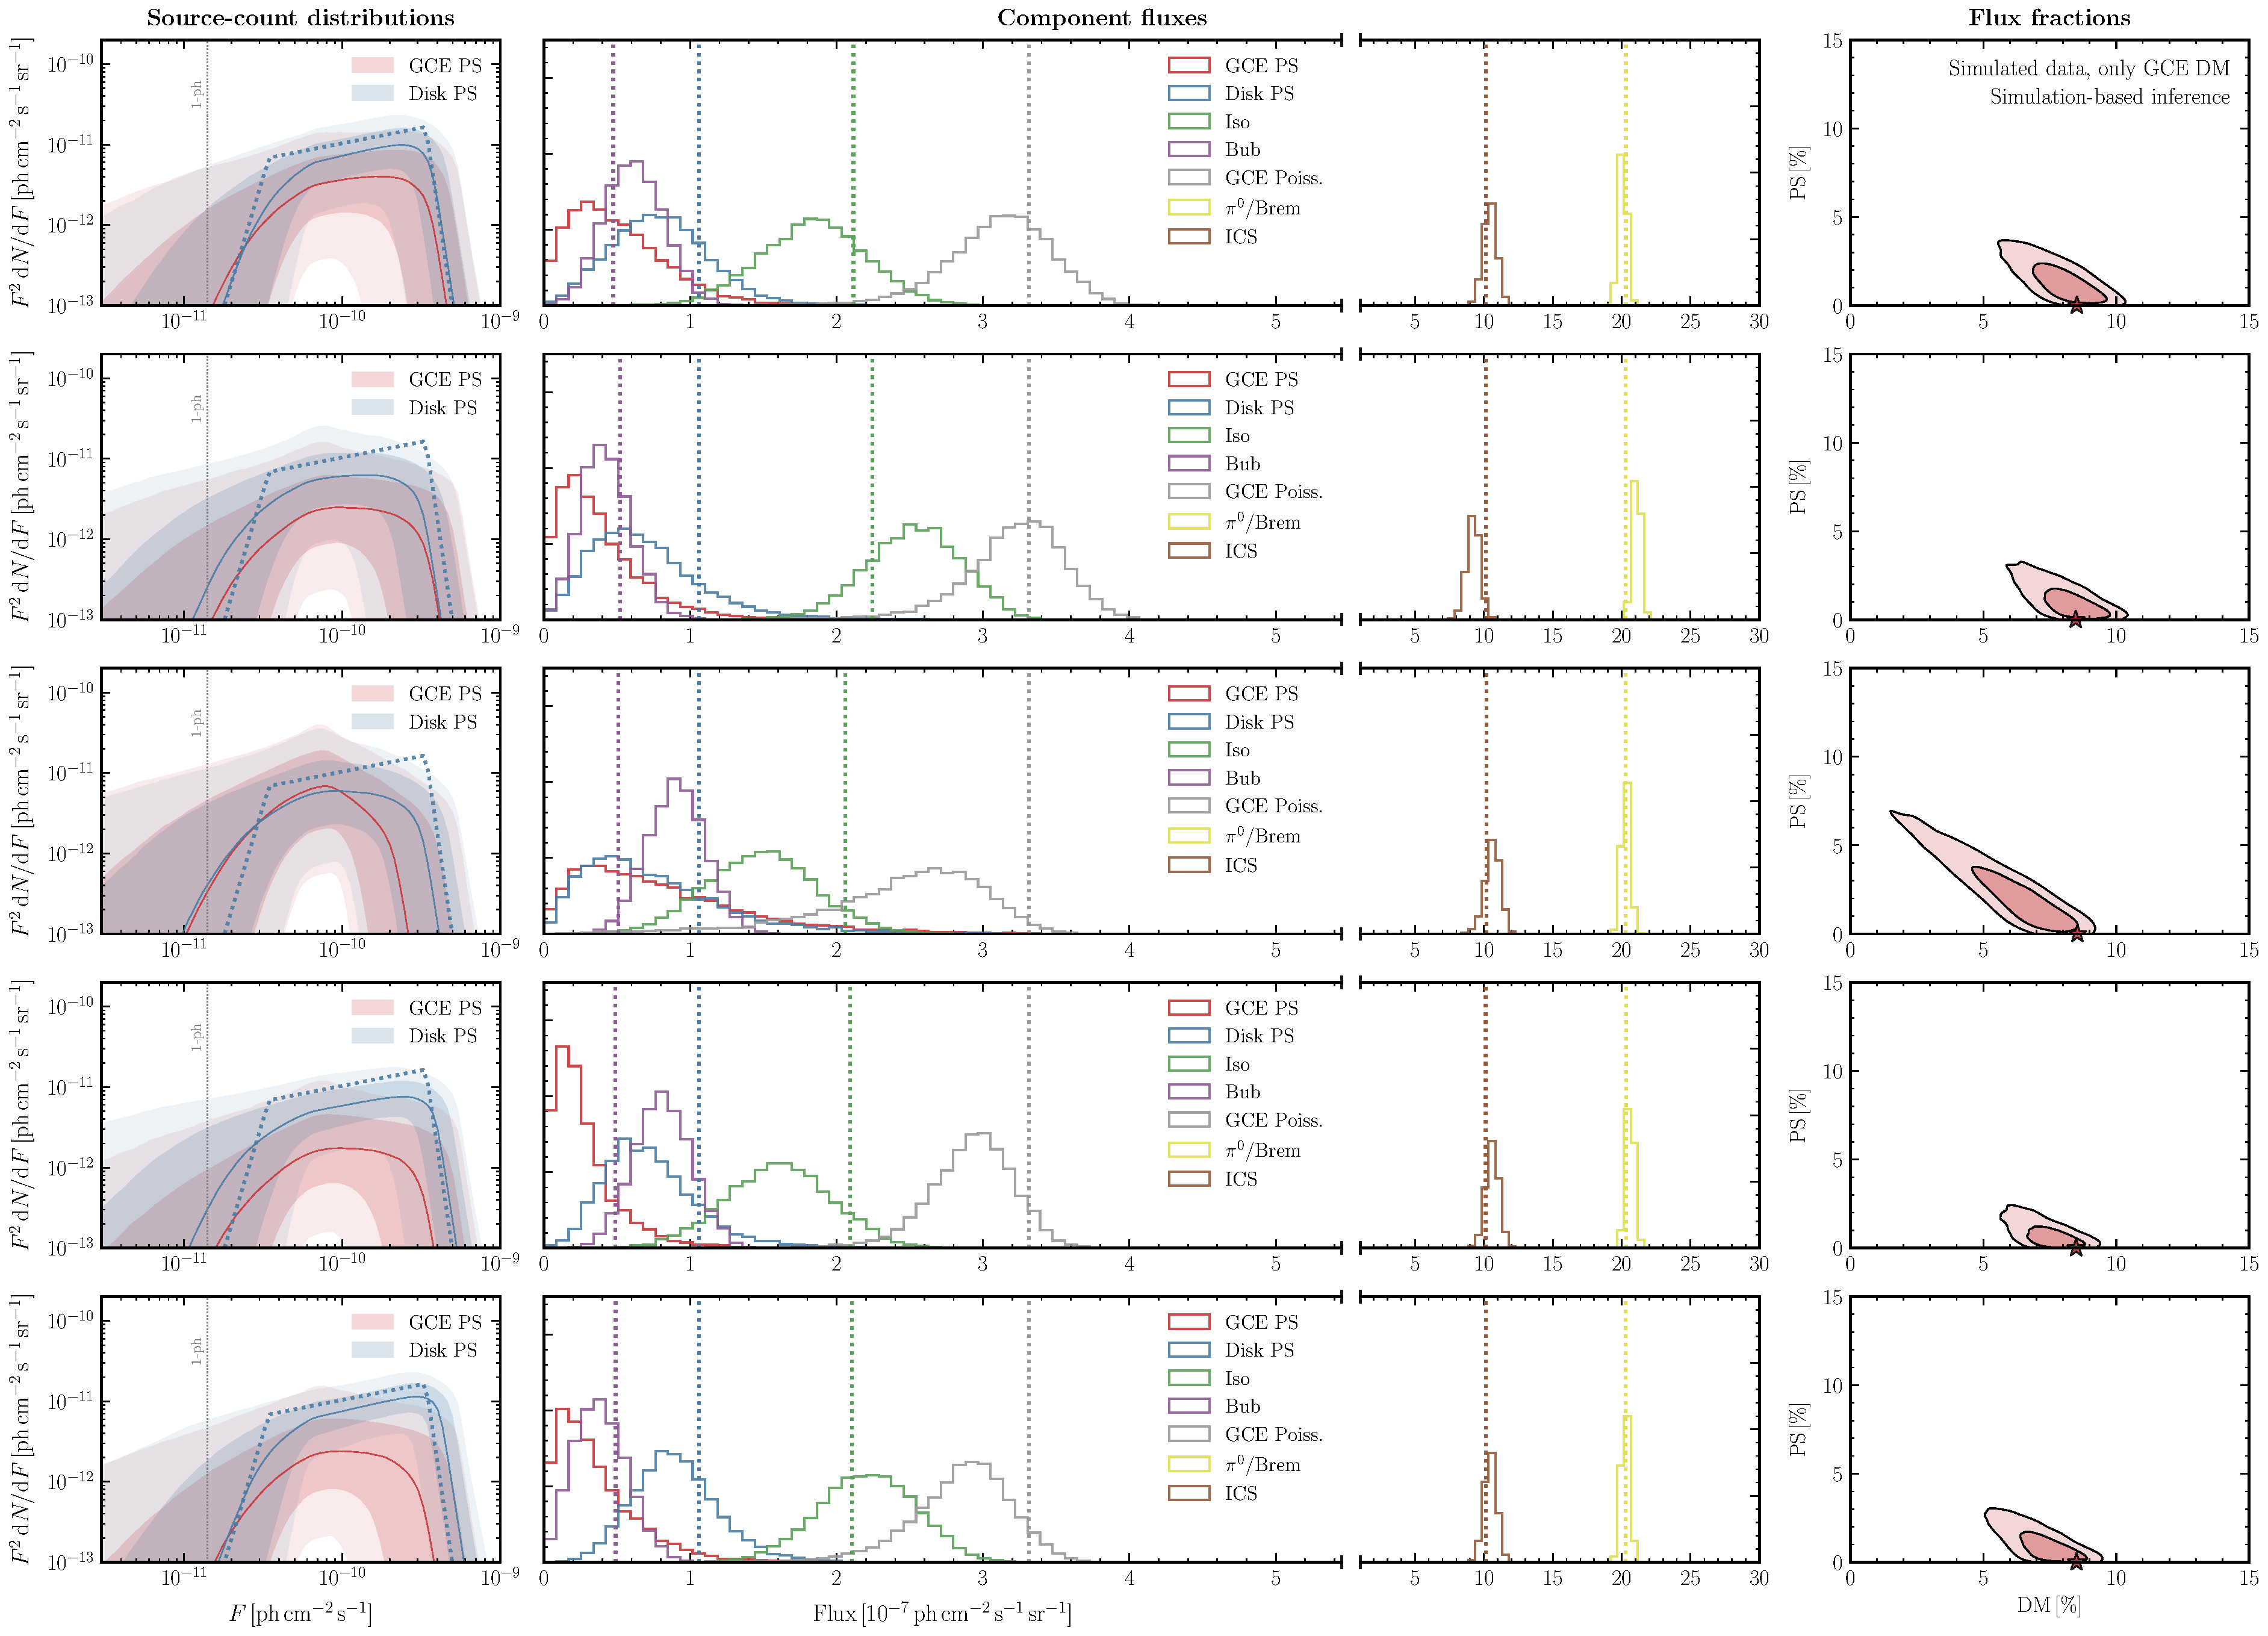
\includegraphics[width=0.95\textwidth]{plots/sim_sbi_dm.pdf}
\caption{Results of the analysis pipeline on simulated \Fermi data where the GCE consists of purely DM-like emission, with different rows corresponding to five different simulated realizations. The left column shows the inferred source-count distribution posteriors for GCE-correlated (red) and disk-correlated (blue) PS. Dashed vertical lines corresponding to the flux associated with 1 expected photon count per source and the approximate 1-$\sigma$ threshold for detecting individual sources are given for reference. Solid lines correspond to the inferred point-wise median, with the lighter and darker bands representing the point-wise middle-68\% and 95\% posterior containment respectively. The middle panel shows the posteriors for the Poissonian templates. The right panel shows the joins posterior on the flux fractions of DM-like and PS-like emission. The dotted lines (in the left two columns) and the stars (in the right column) correspond to the true simulated quantities. DM-like emission is successfully inferred in each case, with the other parameter posteriors corresponding faithfully to the true simulated values.} 
\label{fig:sim_sbi_dm}
\end{figure*}
%

\section{Tests on simulated data}
\label{sec:simulations}

We begin by validating our pipeline on simulated \Fermi data. We create simulated datasets by drawing parameter values from ranges motivated by a fit of the model to real \Fermi data in our fiducial ROI, and test the ability of our model to infer the presence of either DM-like or PS-like signals on top of the modeled astrophysical background.

Figure~\ref{fig:sim_sbi_dm} shows results of the analysis pipeline conditioned on five simulated realizations of maps where the GCE consists of purely DM-like emission. The left column shows the middle-68/95\% containment of the point-wise posterior on the source-count distributions of GCE- and disk-correlated point source emission in red and blue, respectively. The dashed grey vertical lines correspond to the flux associated with a single expected photon count per source (below which Poissonian and PS-like emission is expected to be perfectly degenerate) and the approximate 1-$\sigma$ threshold for detecting individual sources (below which the degeneracy is often empirically observed in practice when using 1-point PDF likelihood-based methods~\cite{Chang:2019ars,Buschmann:2020adf}). The middle column shows the posteriors on various modeled emission components, excluding emission from resolved 3FGL PSs as the posterior in that case is largely unconstrained owing to the fact that resolved PSs are masked out in the analysis. The right column shows the fraction of DM- and PS-like emission in proportion to the total inferred flux in the ROI. The true underlying parameter values from which the data was generated are represented by dotted lines in the left and middle columns, and by star markers in the right column. We see that, in all cases shown, the pipeline successfully recovers the presence of DM-like emission, with little flux attributed to unresolved PSs. Some PS-like emission is inferred in most cases as well however, due to a combination of degeneracy with both disk-correlated and DM-like flux. The overall flux of all components corresponds well to their true underlying values.

Figure~\ref{fig:sim_sbi_ps} shows the corresponding results for simulated data containing PS-like emission correlated with the GCE. Here, simulations were produced such that the highest break of the GCE-correlated PS SCD was contained between 5 and 20 expected photon counts, since we found that the method cannot robustly attribute an SCD that corresponds to a peak dimmer than $\lesssim5$ photon counts to a PS population. We see that PS-like emission is successfully inferred in each case, while at the same time exemplifying a degeneracy with the Poissonian component. Furthermore, as seen in the left column, the method is able to characterize the contribution of the two modeled PS components through the inferred source-count distribution. Some degeneracy between GCE- and disk-correlated PSs is seen, although the true SCDs are seen to lie within the 95\% containment interval of the inferred point-wise SCD posteriors in each case.

%
\begin{figure*}
\centering
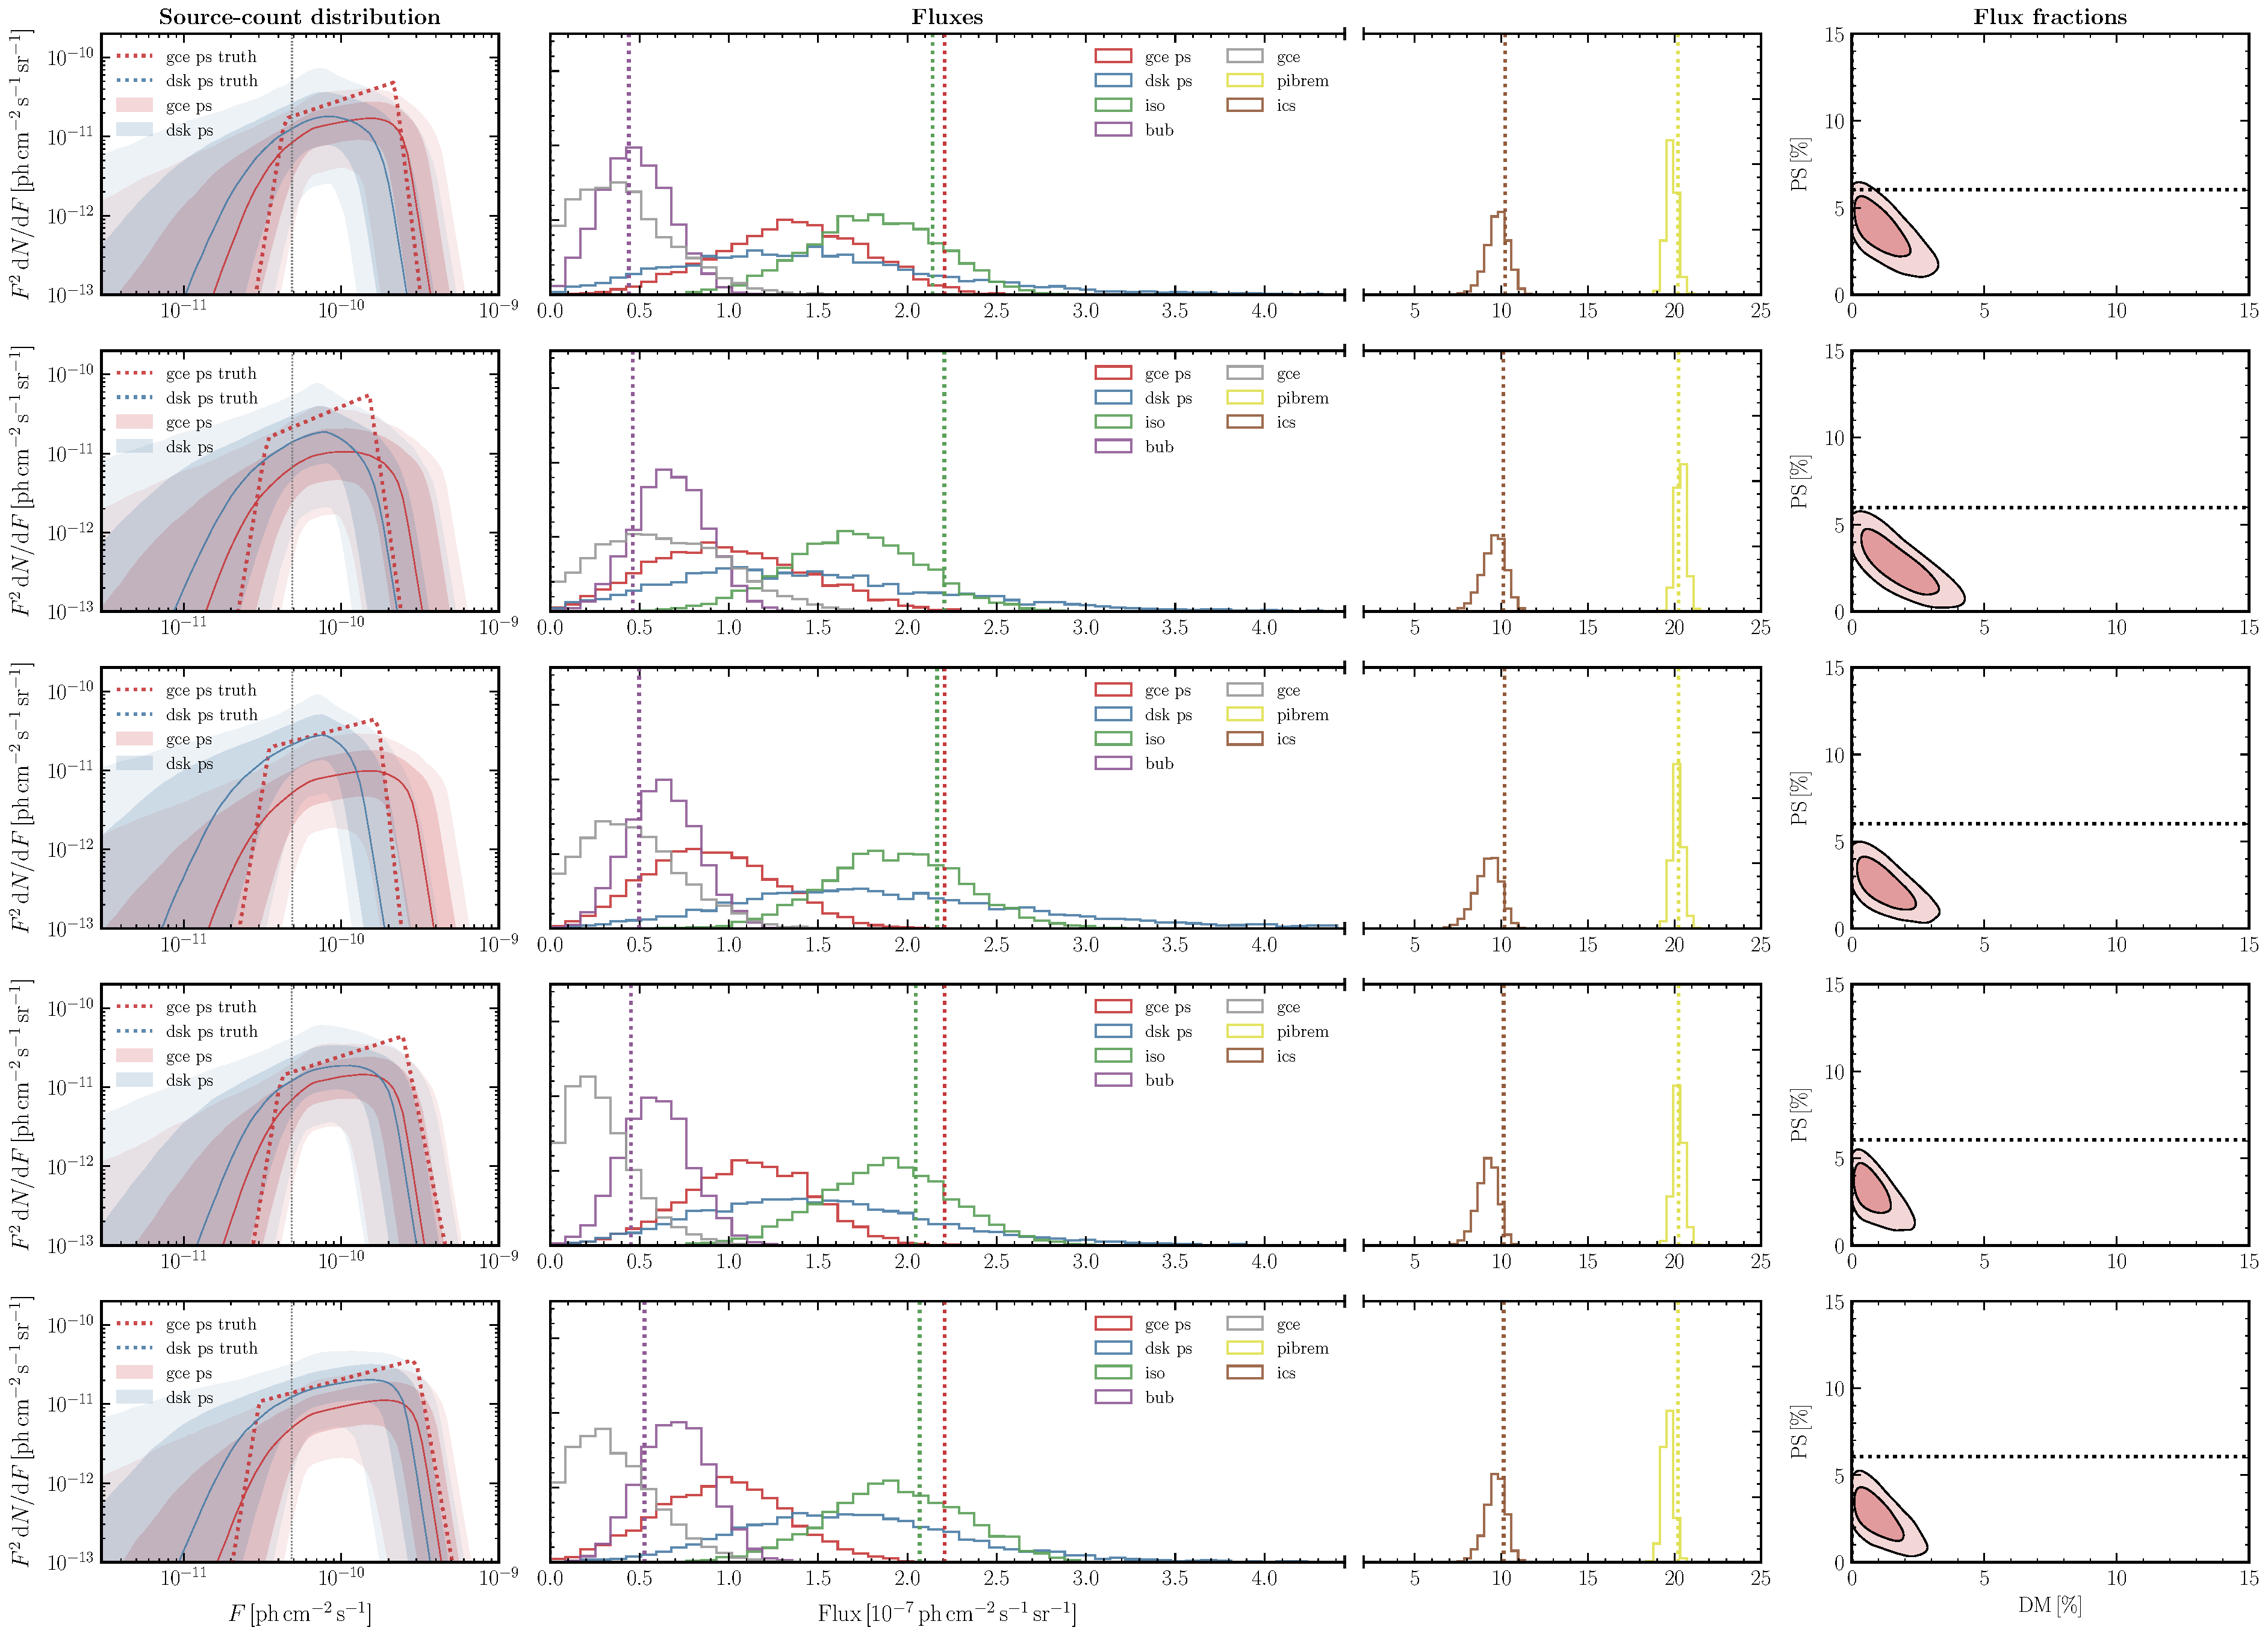
\includegraphics[width=0.95\textwidth]{plots/sim_sbi_ps.pdf}
\caption{Same as Fig.~\ref{fig:sim_sbi_dm}, but for five simulated realization of \Fermi data where the GCE consists of predominantly PS-like emission. PS-like emission is inferred in each case, with the other posteriors corresponding faithfully to their true simulated quantities. The GCE-correlated source-count distribution is also seen to be successfully recovered in the left panel.}
\label{fig:sim_sbi_ps}
\end{figure*}
%

\section{Results on \emph{Fermi} data}
\label{sec:data}

We finally apply our neural simulation-based inference pipeline to the real \Fermi dataset. As a point of comparison, we also run the NPTF pipeline described in Sec.~\ref{sec:likelihood-methods} on the data using the same spatial templates and prior assumptions as those used in the corresponding SBI analyses. A summary of the results obtained for the various analysis configurations explored, for both the SBI and NPTF pipelines, is shown in Table~\ref{tab:results}, including the fraction of overall emission attributed to the GCE, fraction of the GCE attributed to PS-like emission, flux at which the GCE source count distribution peaks, fraction of the overall emission attributed to disk-correlated PSs, and flux at which the disk source count distribution peaks.

The results of the NPTF analysis are shown in the bottom panel of Fig.~\ref{fig:fid_data}. Consistent with previous studies using a similar configuration, a significant fraction of the GCE---$55.0^{+8.8}_{-22.9}\%$--is attributed to PS-like emission.
The top panel of Fig.~\ref{fig:fid_data} shows results using the neural simulation-based analysis pipeline introduced in this paper. Although posteriors for the astrophysical background templates are seen to be broadly consistent with the NPTF anlaysis, the preference for PSs is reduced in this case, in comparison, with $30.9^{+8.5}_{-17.9}\%$ of the GCE emission being PS-like. We also note that the inferred GCE-correlated SCD peaks at values lower than those inferred from previous NPTF analyses, which have generally found the bulk of expected emission from PSs to lie just below the 3FGL PS detection threshold~\cite{Lee:2015fea} at $\sim2$--$3\times 10^{-10}$\,ph\,cm$^{-2}$\,s$^{-1}$. In this fiducial configuration, the SCD peak is constrained to be $2.1^{+1.1}_{-2.0}\times 10^{-11}$\,ph\,cm$^{-2}$\,s$^{-1}$. We note that that the position of the SCD peak is related to the flux at which the largest number of PSs are expected to lie, rather than a statement about which fluxes the majority of the emission comes from.


%
\begin{table*}[!t]
    \footnotesize
    \begin{center}
    \begin{tabular}{cc|cccccc}
    \toprule
    \textbf{Configuration}  & \textbf{Method}  & \textbf{GCE fraction}	 & \textbf{GCE PS fraction}  & $F_{\mathrm{peak}}^\mathrm{GCE}$	&  \textbf{Disk PS fraction} &  $F_{\mathrm{peak}}^\mathrm{disk}$	&  \textbf{Posteriors}\Tstrut\Bstrut	\\   
    - & - & - & - & [ph\,cm$^{-2}$\,s$^{-1}$] & - & [ph\,cm$^{-2}$\,s$^{-1}$]	& -\Tstrut\Bstrut	\\   
    \Xhline{1\arrayrulewidth}
    \multirow{2}{*}{Fiducial} & SBI & $7.7^{+0.2}_{-0.6}\%$ & $30.9^{+8.5}_{-17.9}\%$ & $2.1^{+1.1}_{-2.0}$ & $5.1^{+0.5}_{-1.2}\%$ &  $3.7^{+0.9}_{-2.8}$ & \multirow{2}{*}{Figure~\ref{fig:fid_data}}\Tstrut \\
    & NPTF & $7.7^{+0.2}_{-0.6}\%$ & $55.0^{+8.8}_{-22.9}\%$ &  $2.6^{+0.9}_{-1.5}$ & $5.4^{+0.5}_{-1.1}\%$ & $3.7^{+0.9}_{-1.9}$\Bstrut &\\ 
    \hline
    \multirow{2}{*}{Diffuse Model A} & SBI & $6.4^{+0.2}_{-0.6}\%$  & $38.9^{+10.2}_{-21.2}\%$  & $2.5^{+1.3}_{-2.3}$ & $5.6^{+0.4}_{-1.1}\%$ & $2.8^{+1.2}_{-2.4}$ & \multirow{2}{*}{Figure~\ref{fig:fid_data_modelA}}\Tstrut  \\ 
    & NPTF & $6.7^{+0.2}_{-0.6}\%$ & $74.9^{+6.6}_{-22.5}\%$ & $3.0^{+1.0}_{-1.8}$ &  $5.1^{+0.5}_{-1.3}\%$ & $4.3^{+0.6}_{-2.2}$\Bstrut &\\
    \hline
    \multirow{2}{*}{Diffuse Model F} & SBI & $4.7^{+0.2}_{-0.6}\%$ & $52.9^{+10.8}_{-26.1}\%$ & $2.8^{0.9}_{2.5}$ & $4.4^{+0.4}_{-1.0}\%$ & $4.0^{0.9}_{2.6}$
    & \multirow{2}{*}{Figure~\ref{fig:fid_data_modelF}}\Tstrut \\
    & NPTF & $5.2^{+0.2}_{-0.5}\%$ & $67.5^{+8.6}_{-26.7}\%$ & $3.0^{1.0}_{2.0}$ & $6.4^{+0.5}_{-1.1}\%$ & $5.0^{0.4}_{1.9}$\Bstrut &\\
    \hline
    \multirow{2}{*}{Thick disk} & SBI & $8.3^{+0.2}_{-0.6}\%$ & $49.5^{+9.0}_{-22.8}\%$ & $2.5^{+1.0}_{-2.2}$ & $2.8^{+0.5}_{-1.2}\%$ &  $3.0^{+1.0}_{-2.6}$ & \multirow{2}{*}{Figure~\ref{fig:fid_data_thick_disk}}\Tstrut \\
    & NPTF & $8.2^{+0.3}_{-0.7}\%$ & $75.0^{+7.1}_{-22.6}\%$ & $3.0^{+1.0}_{-1.8}$ & $2.3^{+0.7}_{-1.1}\%$ & $3.0^{+1.0}_{-2.0}$\Bstrut &\\
    \botrule
    \end{tabular}
    \end{center}
    \caption{Parameter priors used for the components of the forward model described in Sec.~\ref{sec:datasets}. All priors are uniform within the ranges specified. Priors on the Poissonian components, corresponding to overall normalization, are shown in the left table column, while those of the GCE- and disk-correlated PS components, parameterized according to Eq.~\eqref{eq:scd_bpl}, are shown in the right table column. The overall normalizations of the Poissonian GCE and PS-like components are parameterized through the mean number of counts contributed by the respective components in the ROI.}
    \label{tab:results}
    \end{table*}    
    %

%
\begin{figure*}
\centering
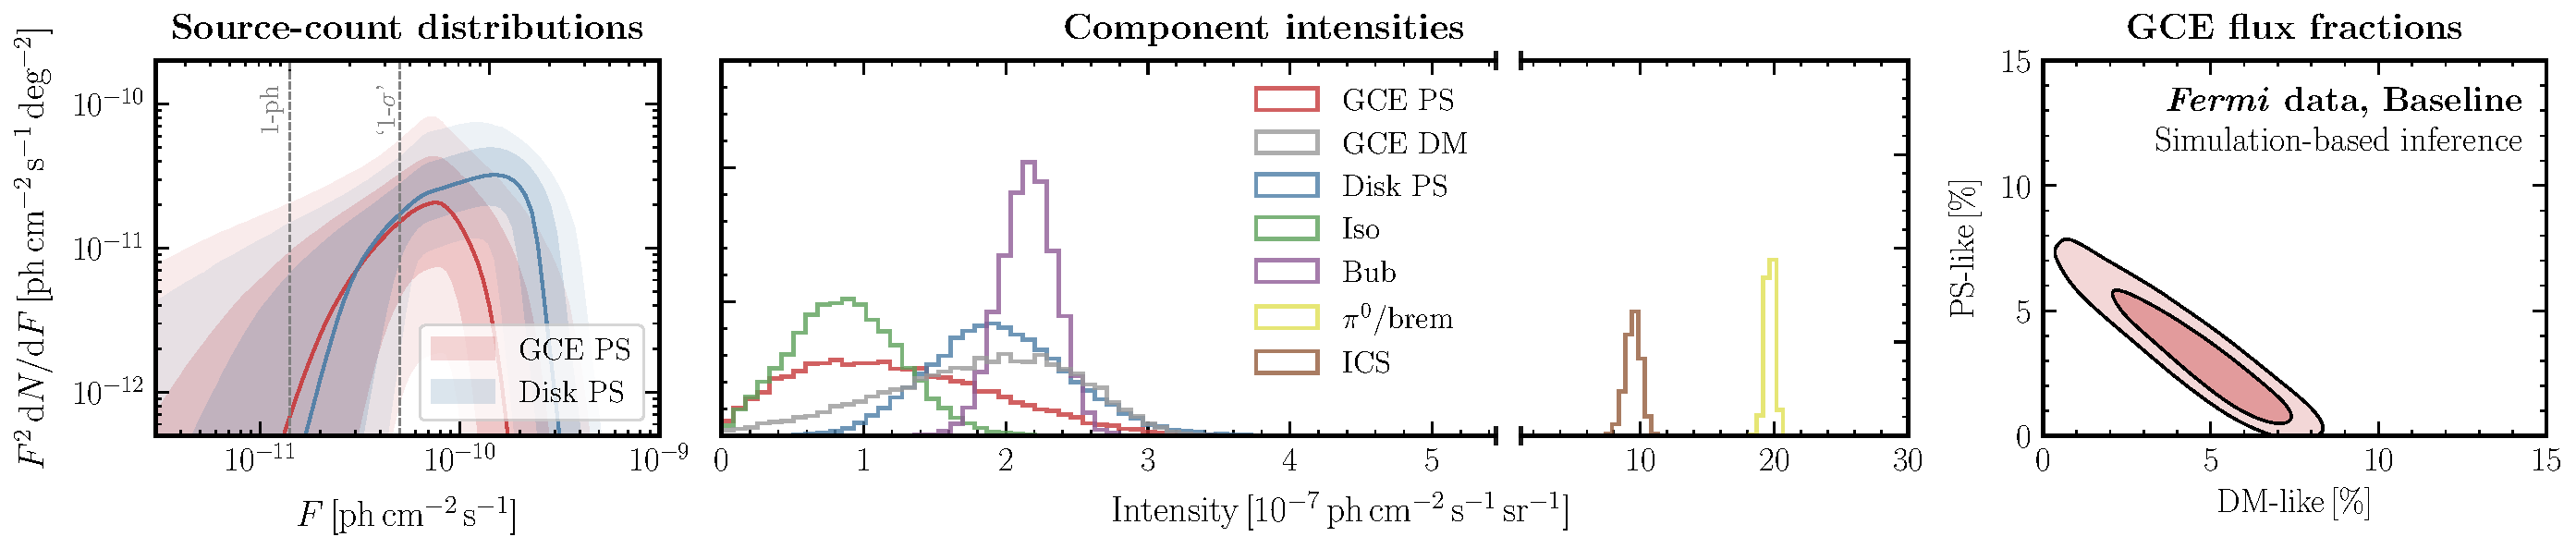
\includegraphics[width=0.95\textwidth]{plots/data_fid_sbi.pdf}
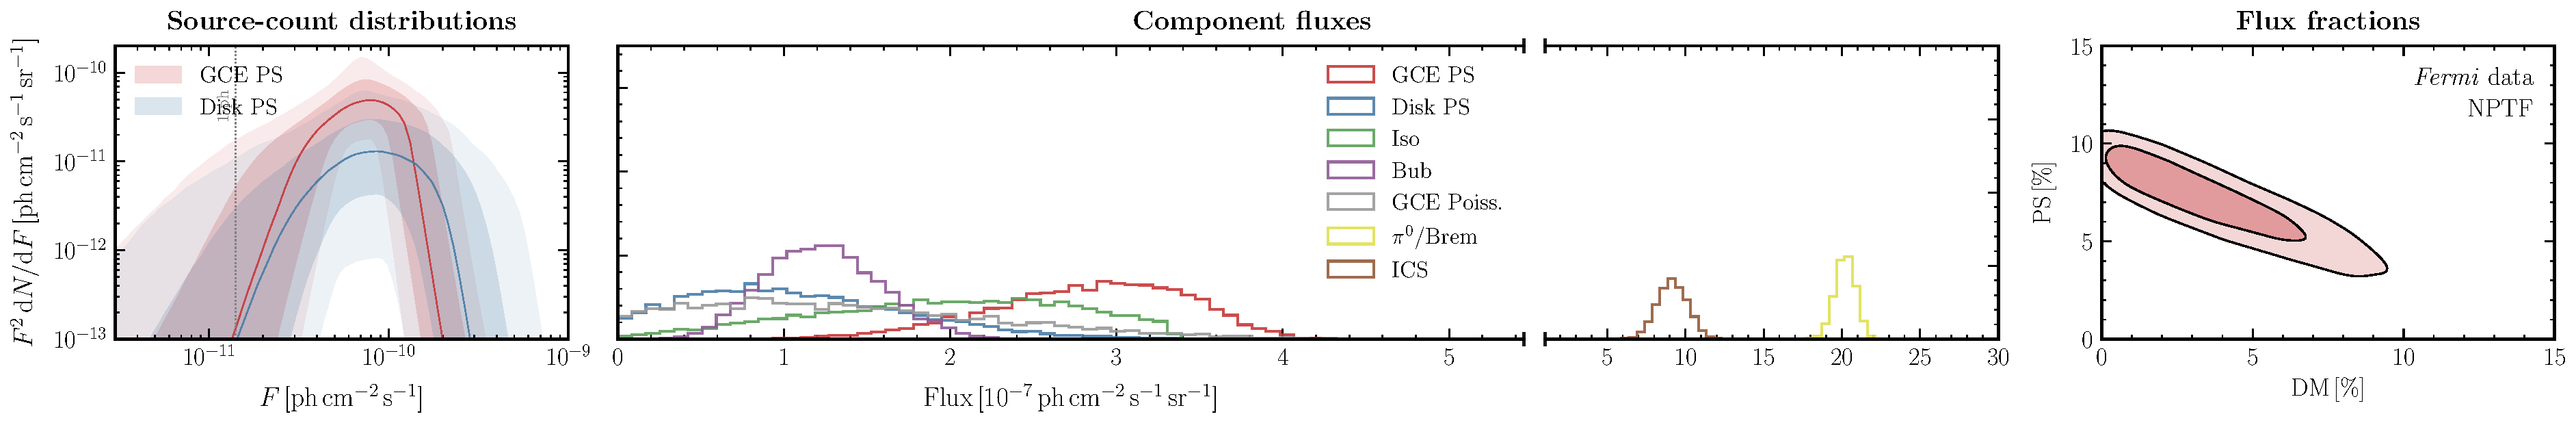
\includegraphics[width=0.95\textwidth]{plots/data_fid_nptf.pdf}
\caption{Results of the fiducial analysis on real \Fermi data. \emph{(Top row)} Analysis using neural simulation-based inference with normalizing flows, and \emph{(bottom row)} using the 1-point PDF likelihood implemented in the non-Poissonian template fitting (NPTF) framework. While moderate preference for a PS-like origin of the GCE is seen in the case of the NPTF analysis (bottom), the simulation-based inference analysis attributes a smaller fraction of the GCE to PS-like emission (top).}
\label{fig:fid_data}
\end{figure*}
%

\subsection{Signal injection test on data}
\label{sec:sig-injection}

A crucial self-consistency test is the ability of the analysis to recover an artificial signal injected onto the real $\gamma$-ray data. As shown in Ref.~\cite{Leane:2019xiy}, early applications of the 1-point PDF based methods like NPTF to the GCE would generally fail this closure test, with implications for characterizing the nature of PSs in the Galactic Center explored in Refs.~\cite{Chang:2019ars,Buschmann:2020adf}. In particular, it was shown that the closure test can help diagnose underlying issues associated with mismodeling of the diffuse foreground emission, which have the potential to bias the characterization of PS populations. We perform a version of this test within our framework, testing the ability of our method to recover different mock signals injection onto the real \Fermi data.

Figure~\ref{fig:sig_inj_data} shows the results of this test, with the different rows corresponding to different signal configuration---purely DM, bright PSs, medium-bright PSs, and dim PSs. Bright, medium-bright, and dim PS configurations are taken to peak at 20, 10, and 5 photon counts respectively. The leftmost columns shows the fiducial analysis on \Fermi data, with subsequent columns showing signals of progressively larger sizes injected onto the data, up to approximately the size of the original GCE signal. The dotted horizontal and vertical lines show the expected total emission on top of the median fluxes for the PS and DM components of the GCE inferred without any additional injected signal, respectively. 

The additional injected signal is seen to be reconstructed correctly within the inferred 95\% confidence interval in all four cases. For the DM signal (top row), the brightest tested DM signal is seen to partially reconstruct as PS-like, which could be attributed to the larger magnitude of Poisson fluctuations in this case mimicking the effect of an unresolved PS population. The injected PS signals (rows 2--4) are correctly reconstructed in all cases, with the dimmer PS signals showing a more prominent flat direction with Poissonian emission, as expected.

%
\begin{figure*}
\centering

\includegraphics[width=0.95\textwidth]{plots/sig_inj_title.pdf}
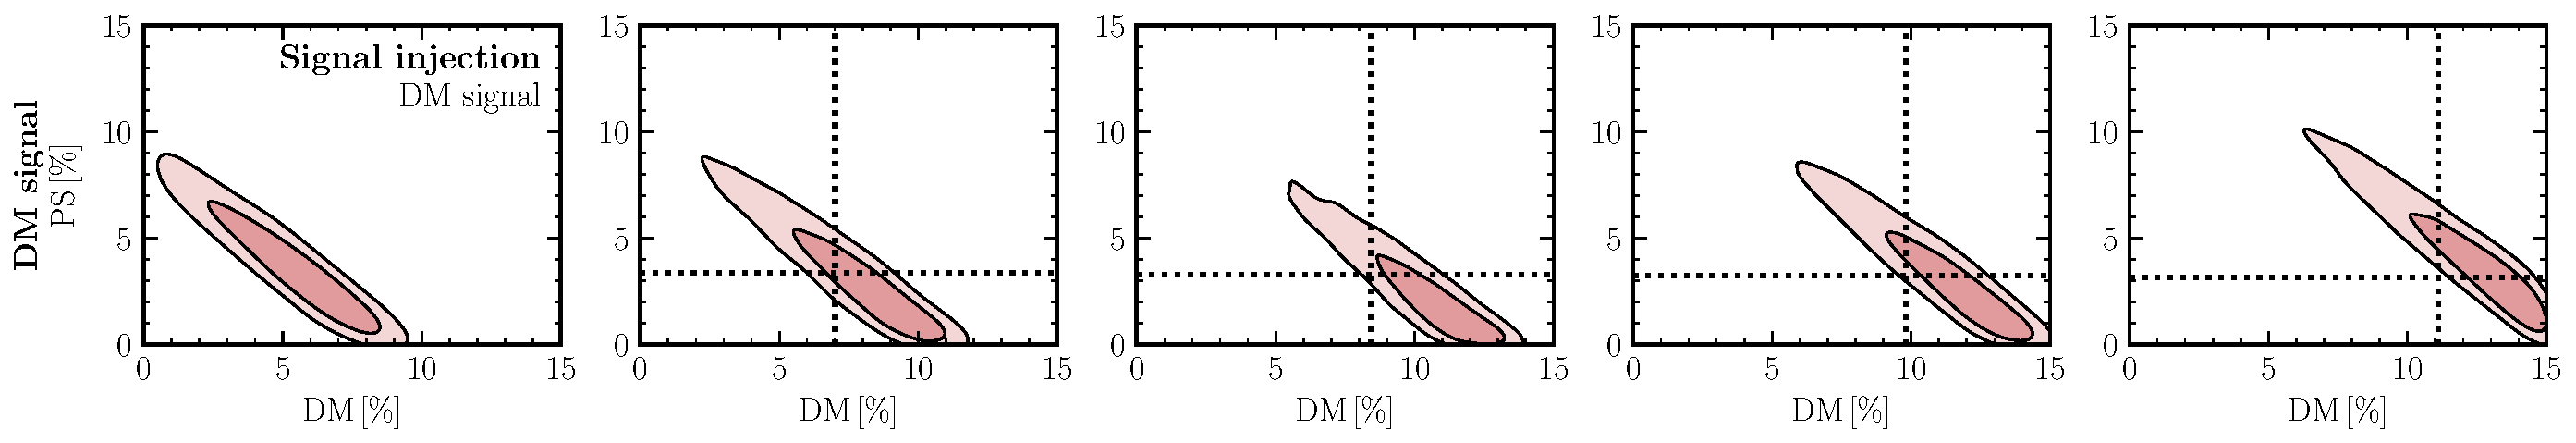
\includegraphics[width=0.95\textwidth]{plots/data_sig_inj_dm.pdf}
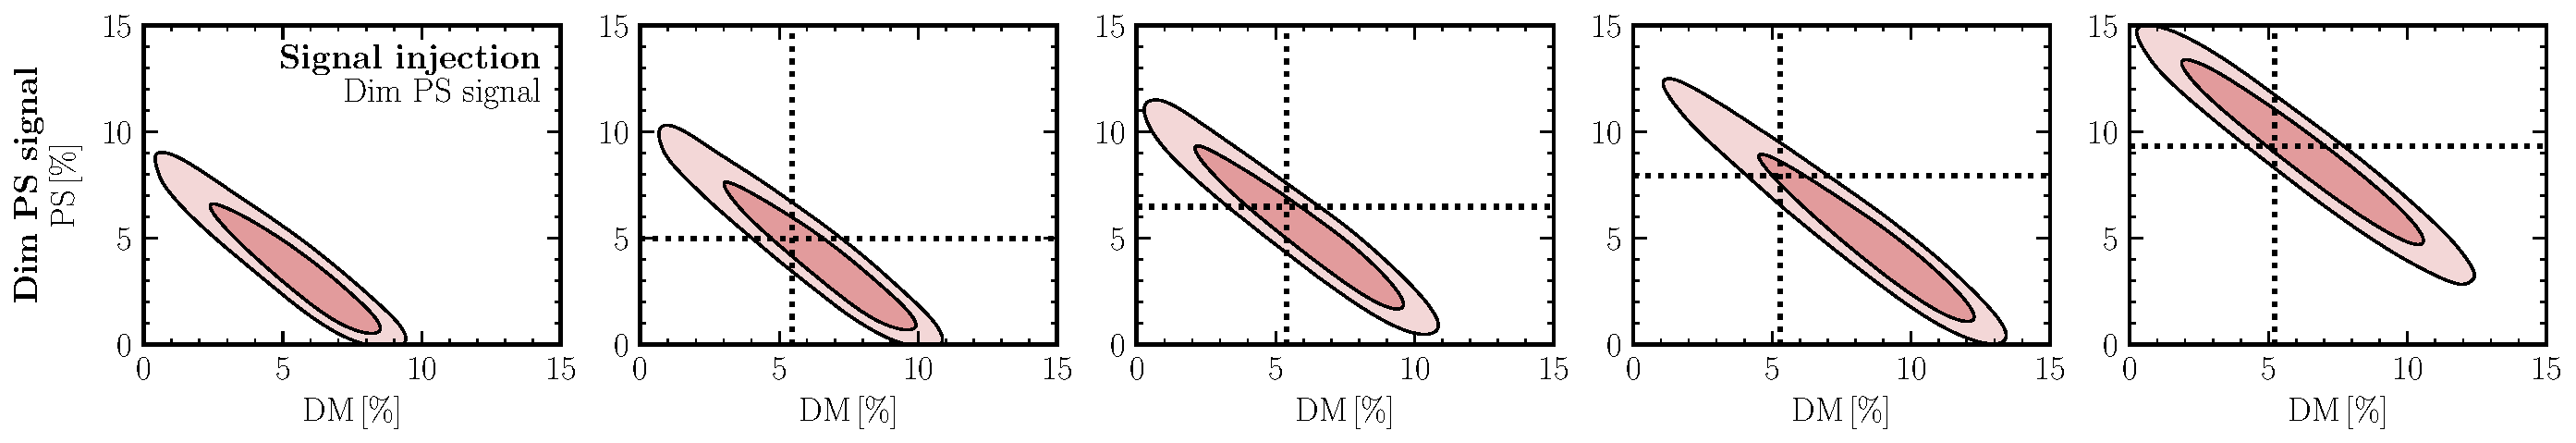
\includegraphics[width=0.95\textwidth]{plots/data_sig_inj_dim_ps.pdf}
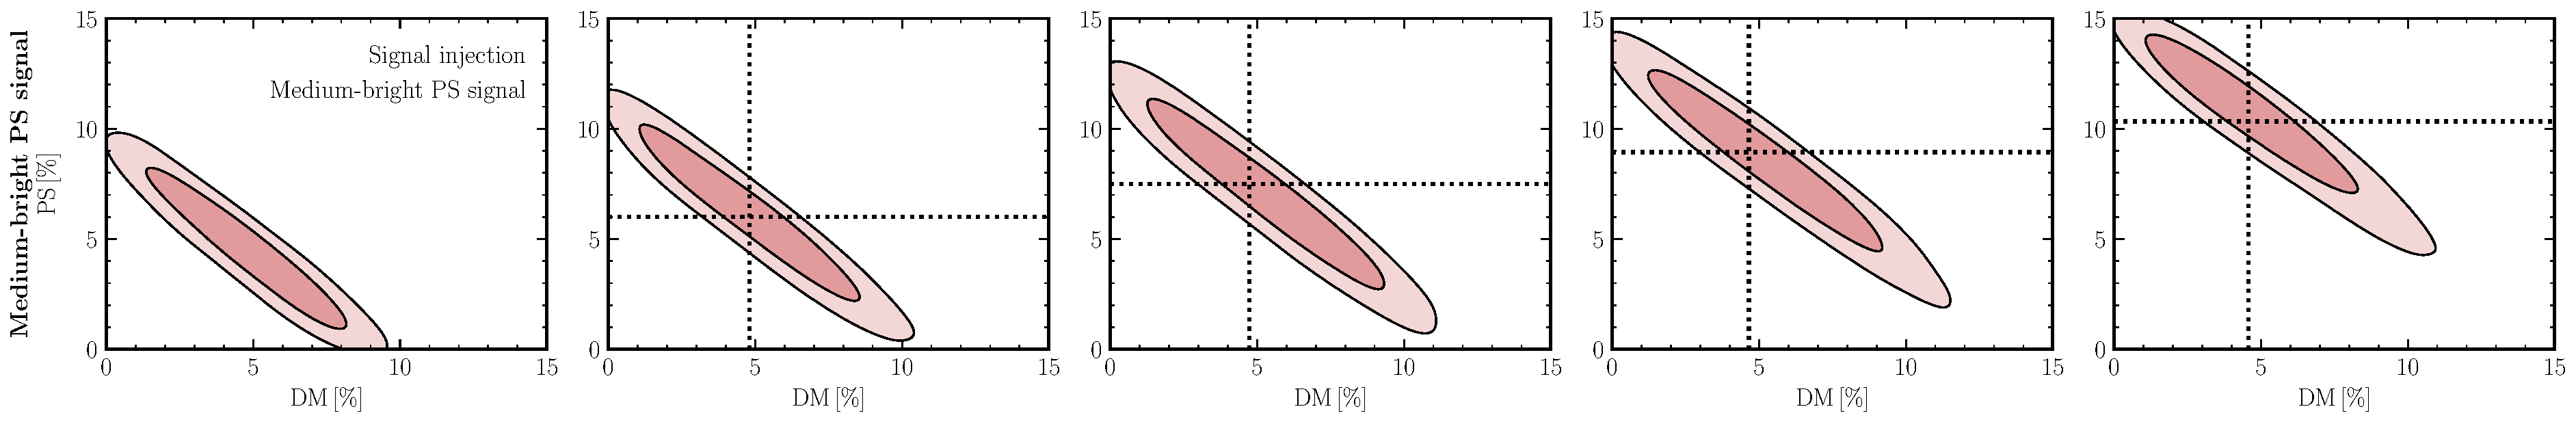
\includegraphics[width=0.95\textwidth]{plots/data_sig_inj_med_ps.pdf}
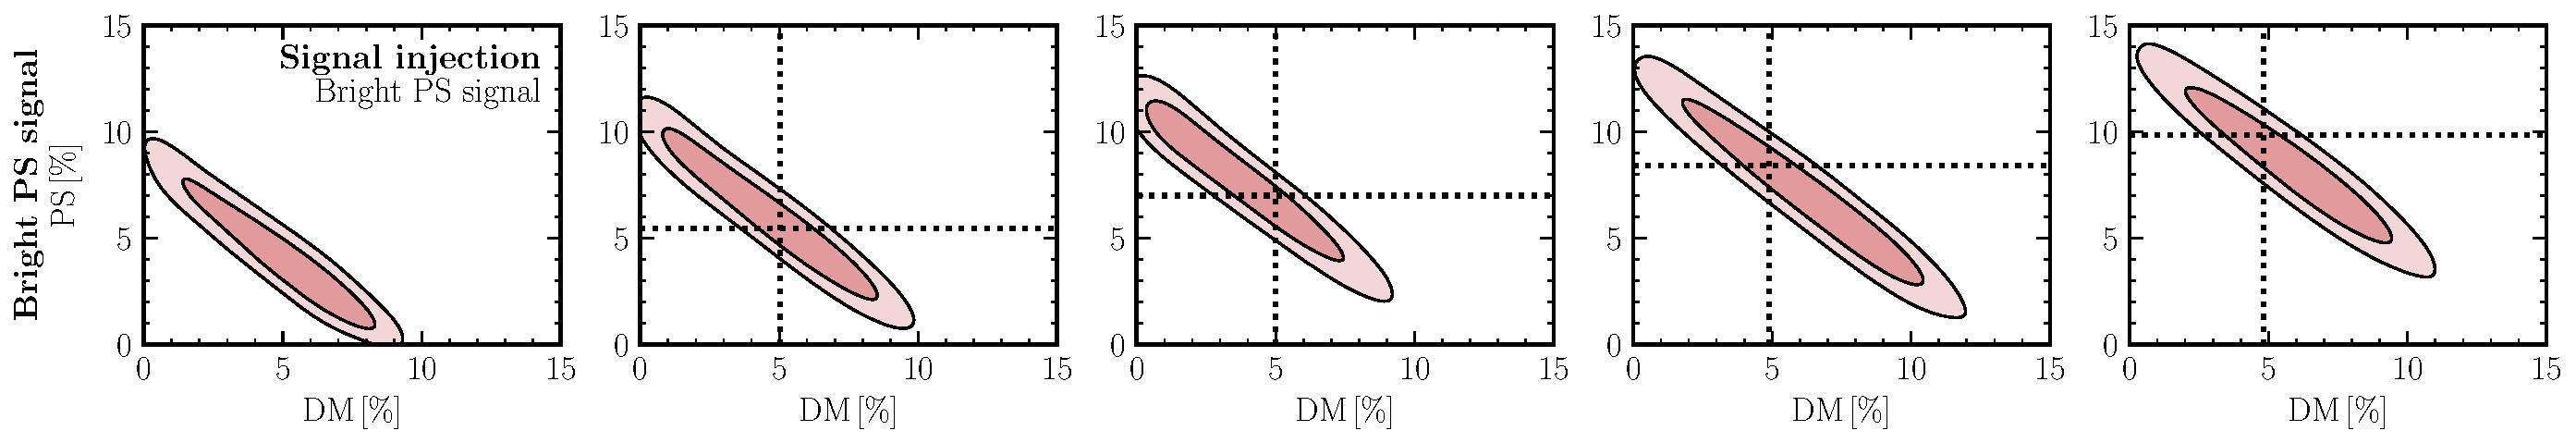
\includegraphics[width=0.95\textwidth]{plots/data_sig_inj_ps.pdf}

\includegraphics[width=0.95\textwidth]{plots/sig_inj_chyron.pdf}
\caption{Joint posterior for the flux fraction of PS-like and DM-like emission when an artificial DM signal is injected onto the real \Fermi data. The different rows correspond to different signal types, from top to bottom, purely DM, dim PSs (maximum of 5 expected counts per PS), moderately-bright PSs (maximum of 10 expected counts per PS), and bright PSs (maximum of 20 expected counts per PS). The leftmost panels shows the fiducial analysis on \Fermi data, with subsequent panels showing results with progressively larger signals injected onto the data. The dotted lines show the expected total emission on top of the median initial inferred flux. The additional injected DM and PS signals are seen to correctly reconstructed within the respective posterior bounds in all cases.}
\label{fig:sig_inj_data}
\end{figure*}
%

\subsection{Systematic variations on the analysis}
\label{sec:systematics}

% %
% \begin{figure*}
%     \centering
%     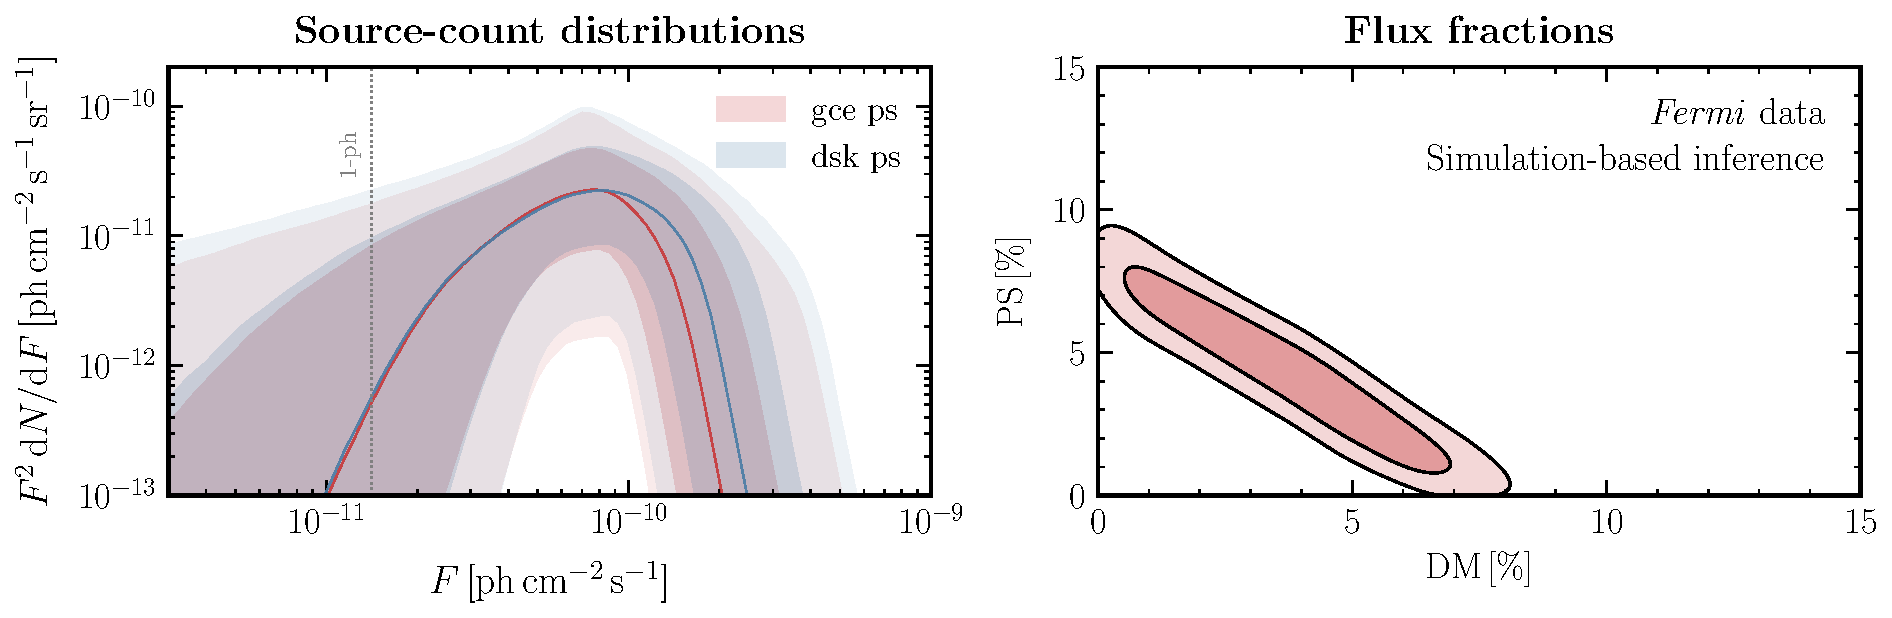
\includegraphics[width=0.45\textwidth]{plots/data_fid_sbi_20.pdf}
%     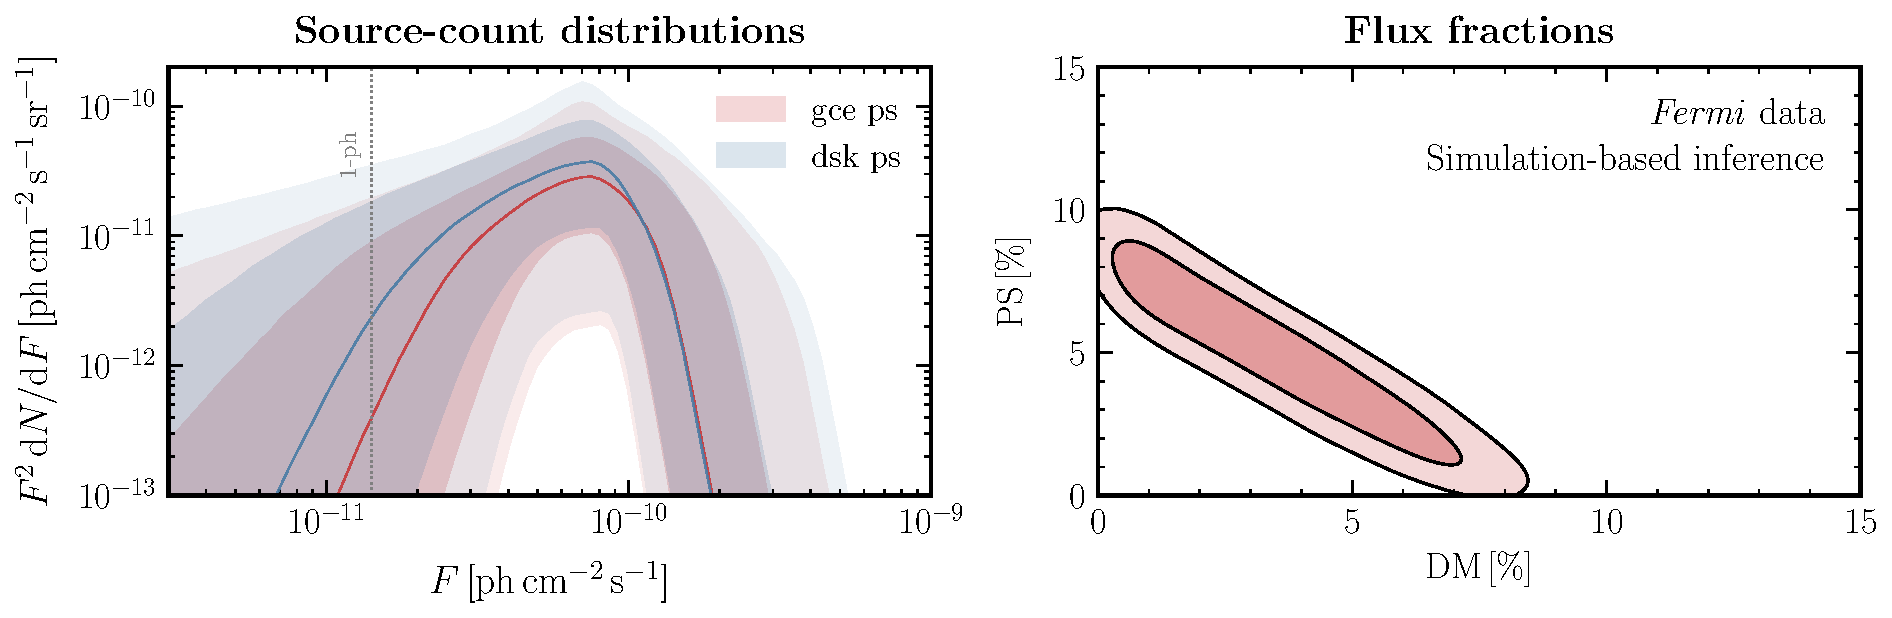
\includegraphics[width=0.45\textwidth]{plots/data_fid_sbi_15.pdf}
%     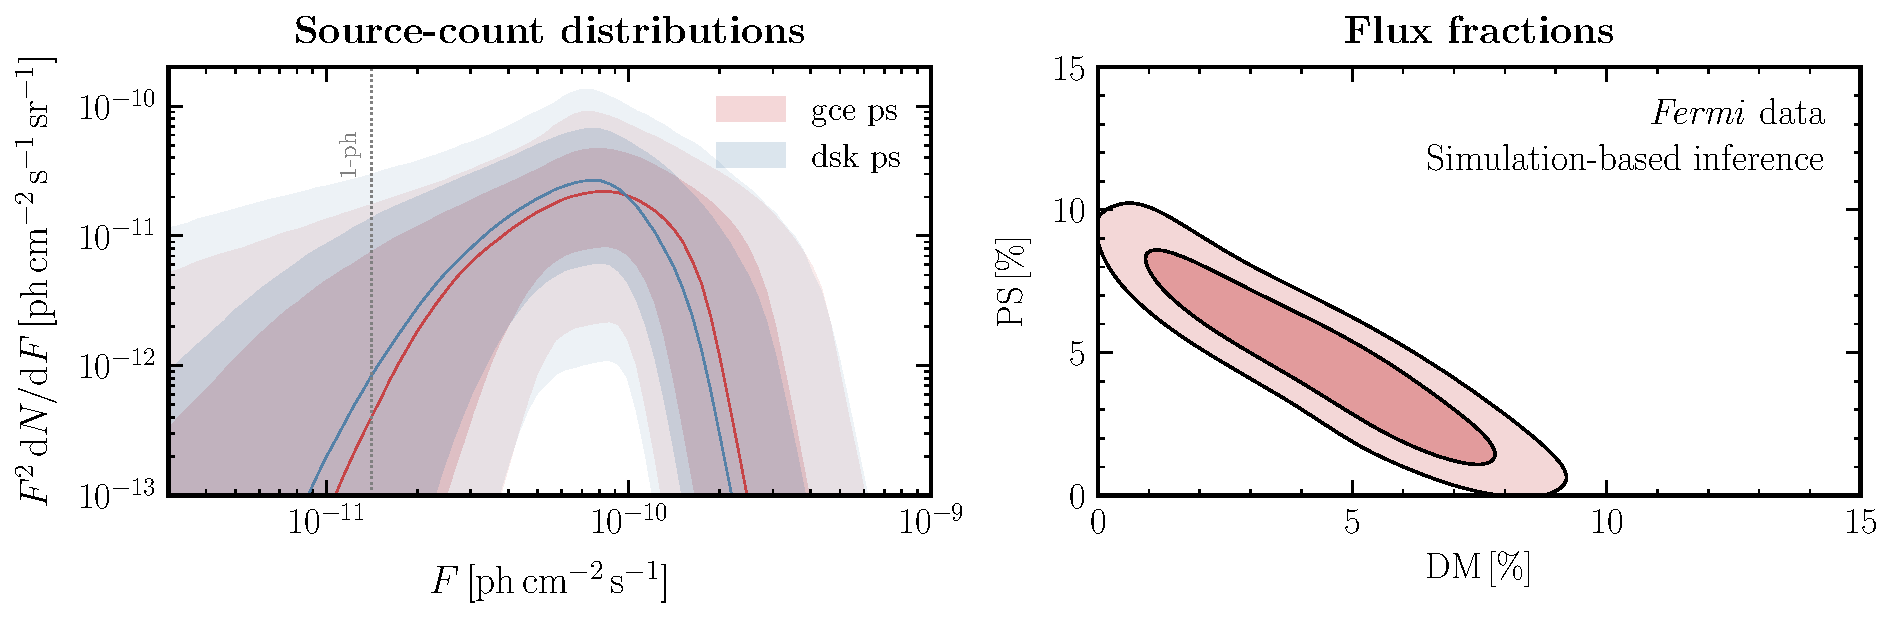
\includegraphics[width=0.45\textwidth]{plots/data_fid_sbi_10.pdf}
%     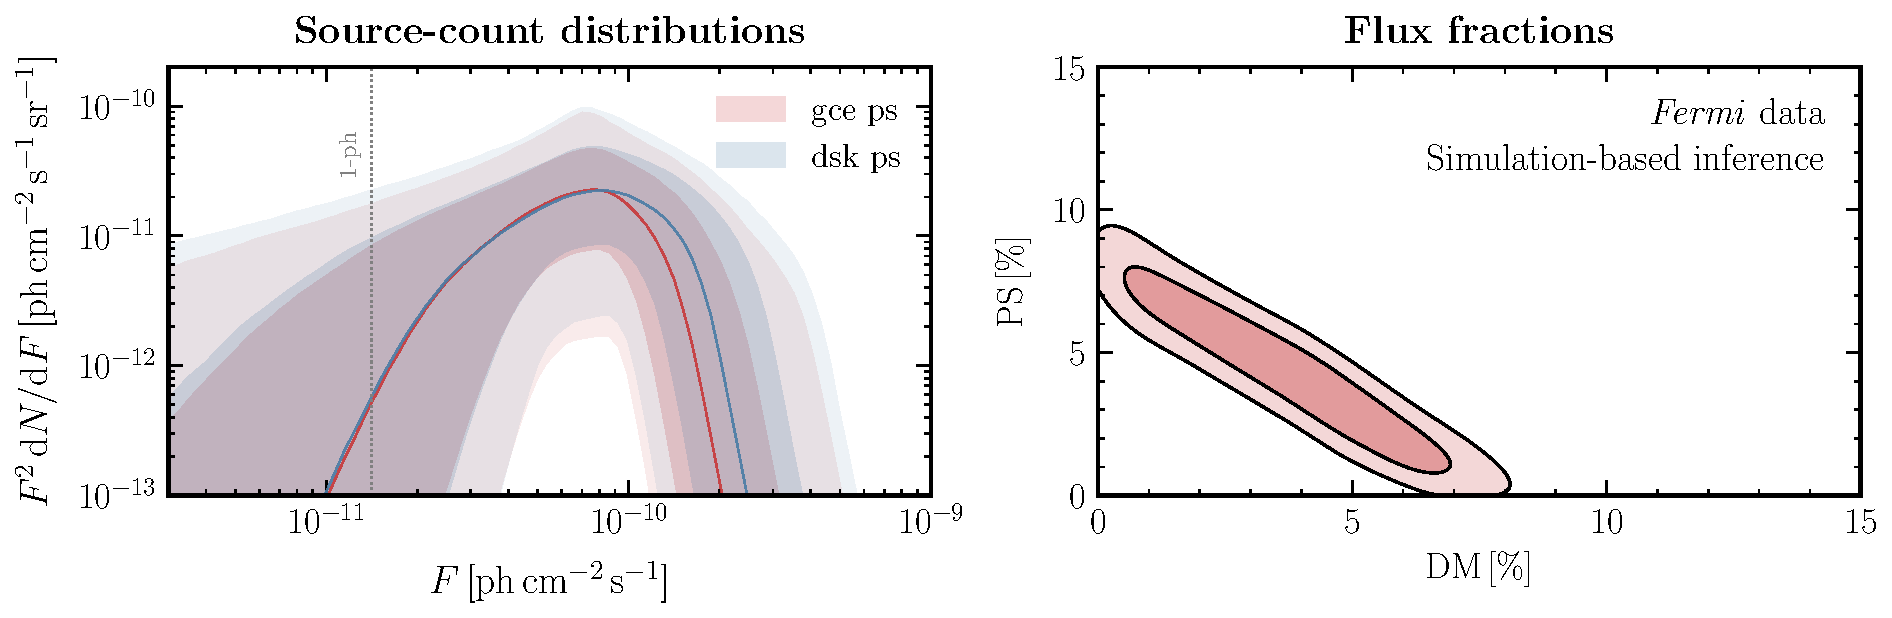
\includegraphics[width=0.45\textwidth]{plots/data_fid_sbi_20.pdf}
%     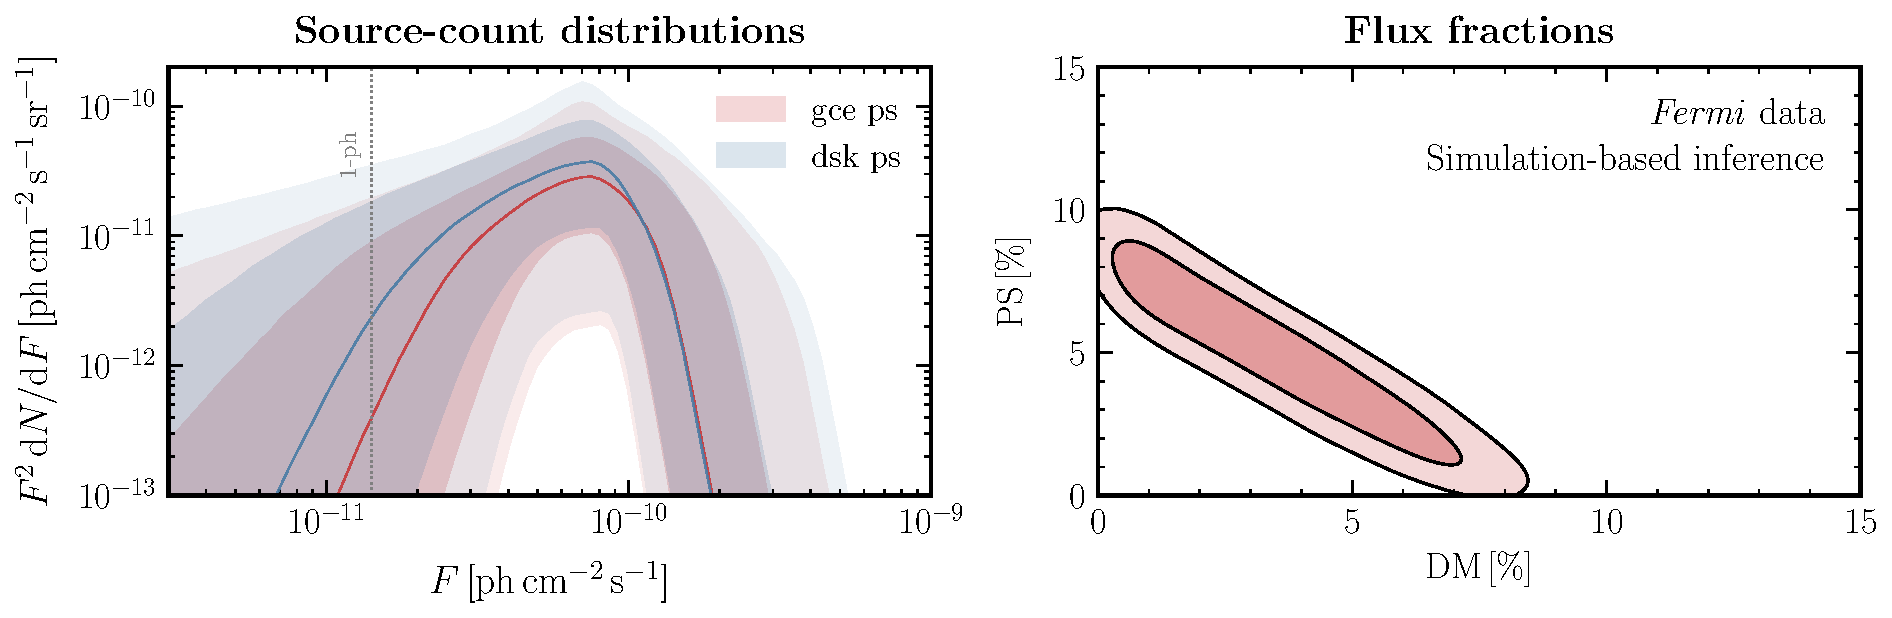
\includegraphics[width=0.45\textwidth]{plots/data_fid_sbi_15.pdf}
%     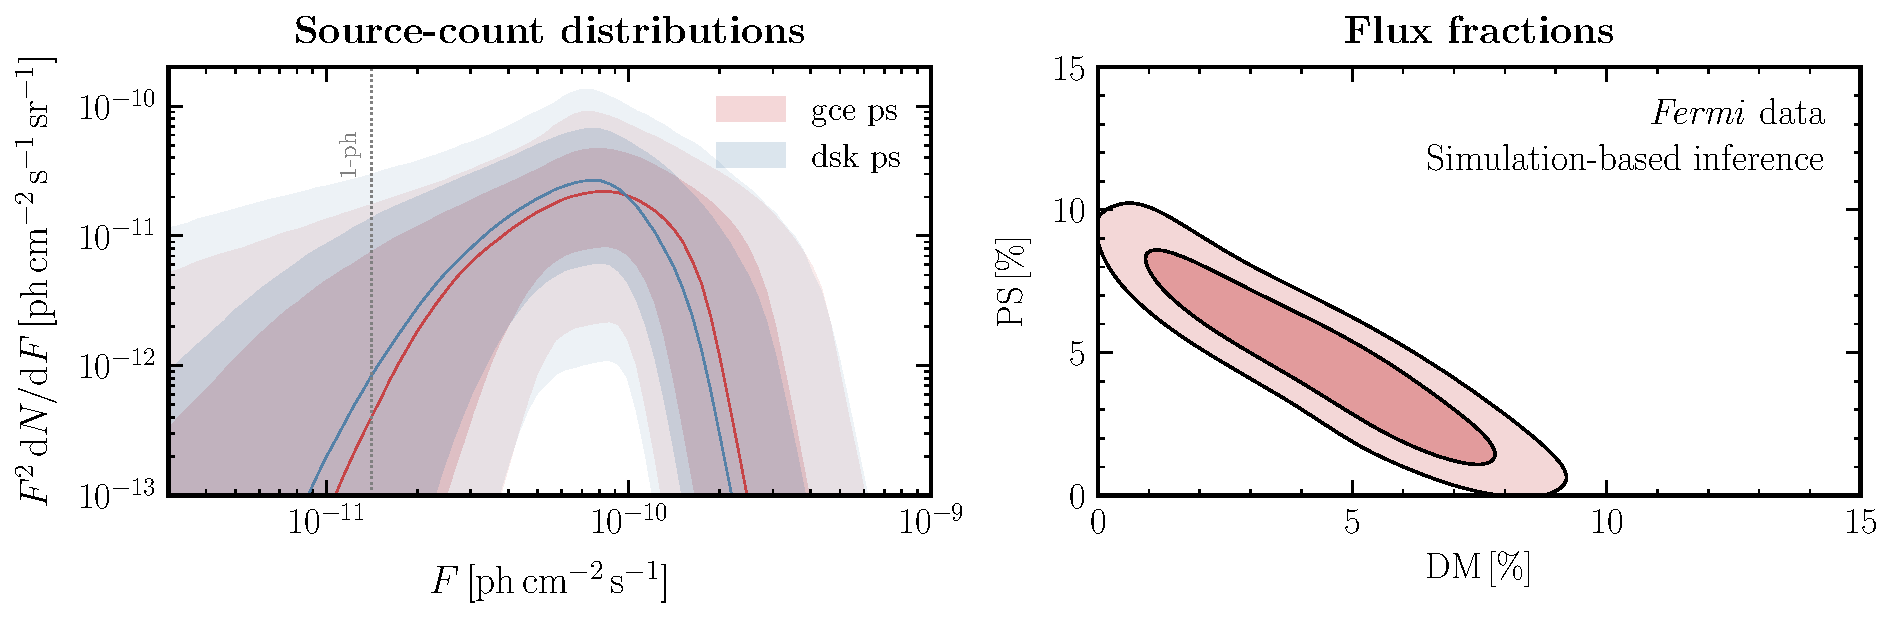
\includegraphics[width=0.45\textwidth]{plots/data_fid_sbi_10.pdf}

%     % 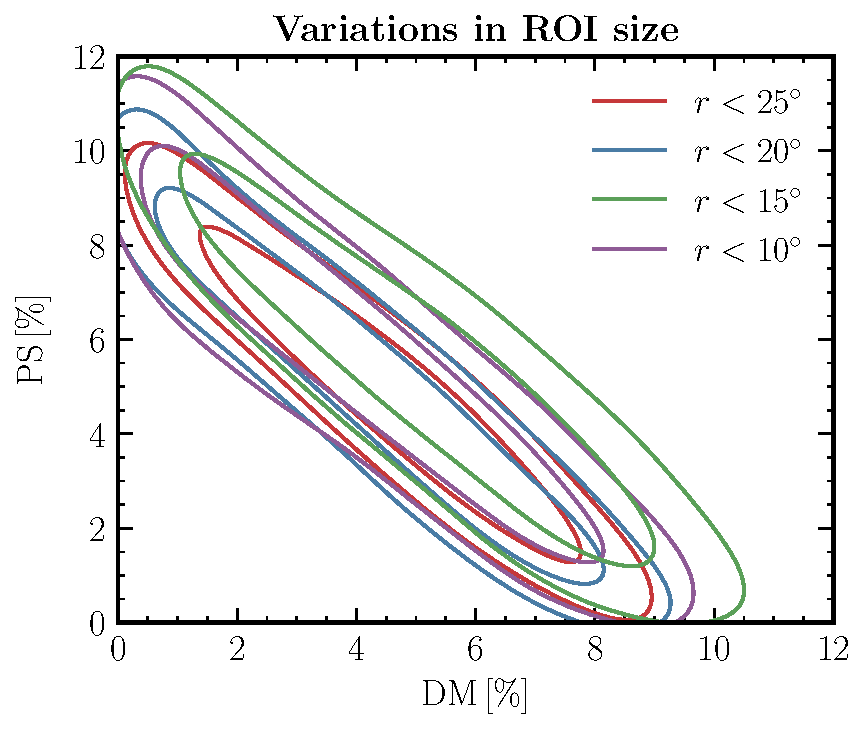
\includegraphics[width=0.22\textwidth]{plots/roi_var.pdf}
%     \caption{Joint posterior for flux fraction of PS-like and DM-like emission on real \Fermi data for different diffuse models \emph{(left)} and ROI sizes \emph{(right)}. In varying diffuse models, the fiducial Model O (red) is compared with results obtained using Models A (blue) and F (green). Although the overall GCE flux is seen to varying by up to a factor of $\sim2$ between diffuse models, no evidence for PS-like emission is seen. As seen in the right panel, results remain consistent for smaller ROI sizes.}
%     \label{fig:variations}
% \end{figure*}
% %



%
\begin{figure*}
\centering
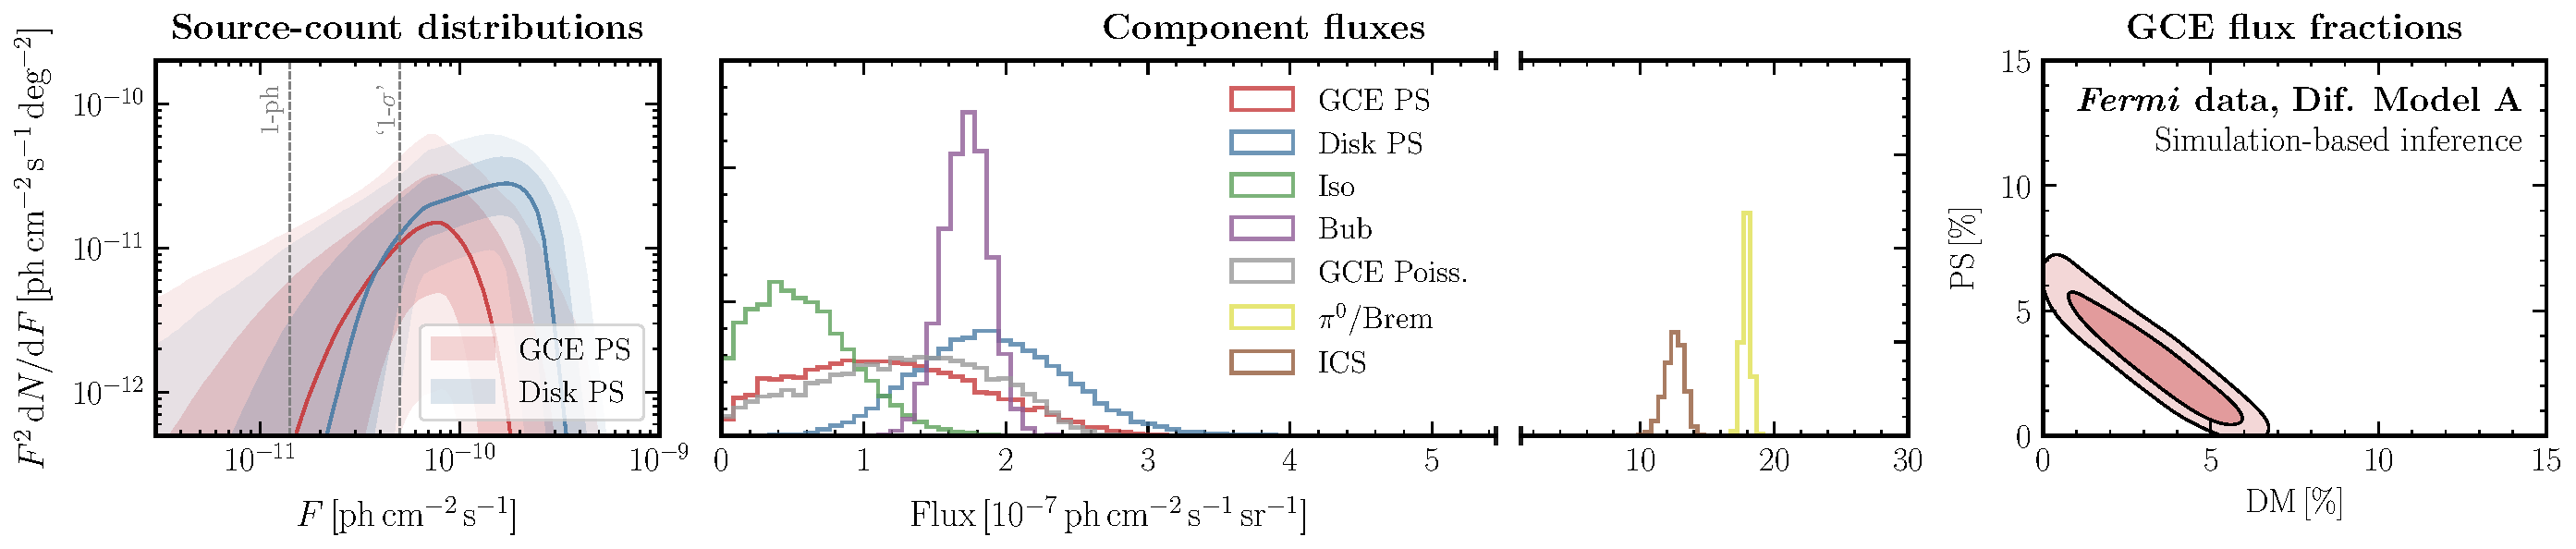
\includegraphics[width=0.95\textwidth]{plots/data_fid_sbi_modelA.pdf}
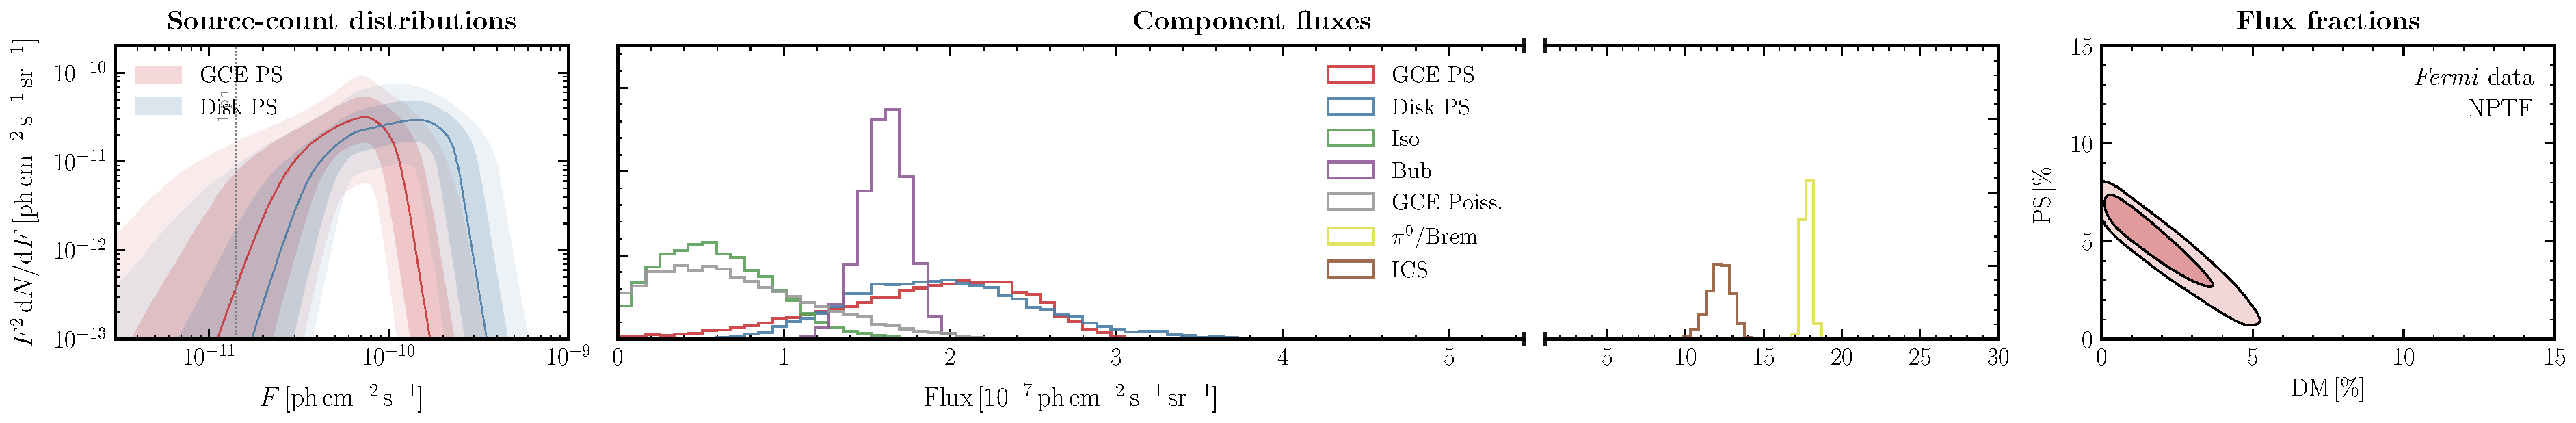
\includegraphics[width=0.95\textwidth]{plots/data_fid_nptf_modelA.pdf}
\caption{Same as Fig.~\ref{fig:fid_data}, but for a model where the diffuse foreground emission is modeled using the alternative Model A.}
\label{fig:fid_data_modelA}
\end{figure*}
%


%
\begin{figure*}
\centering
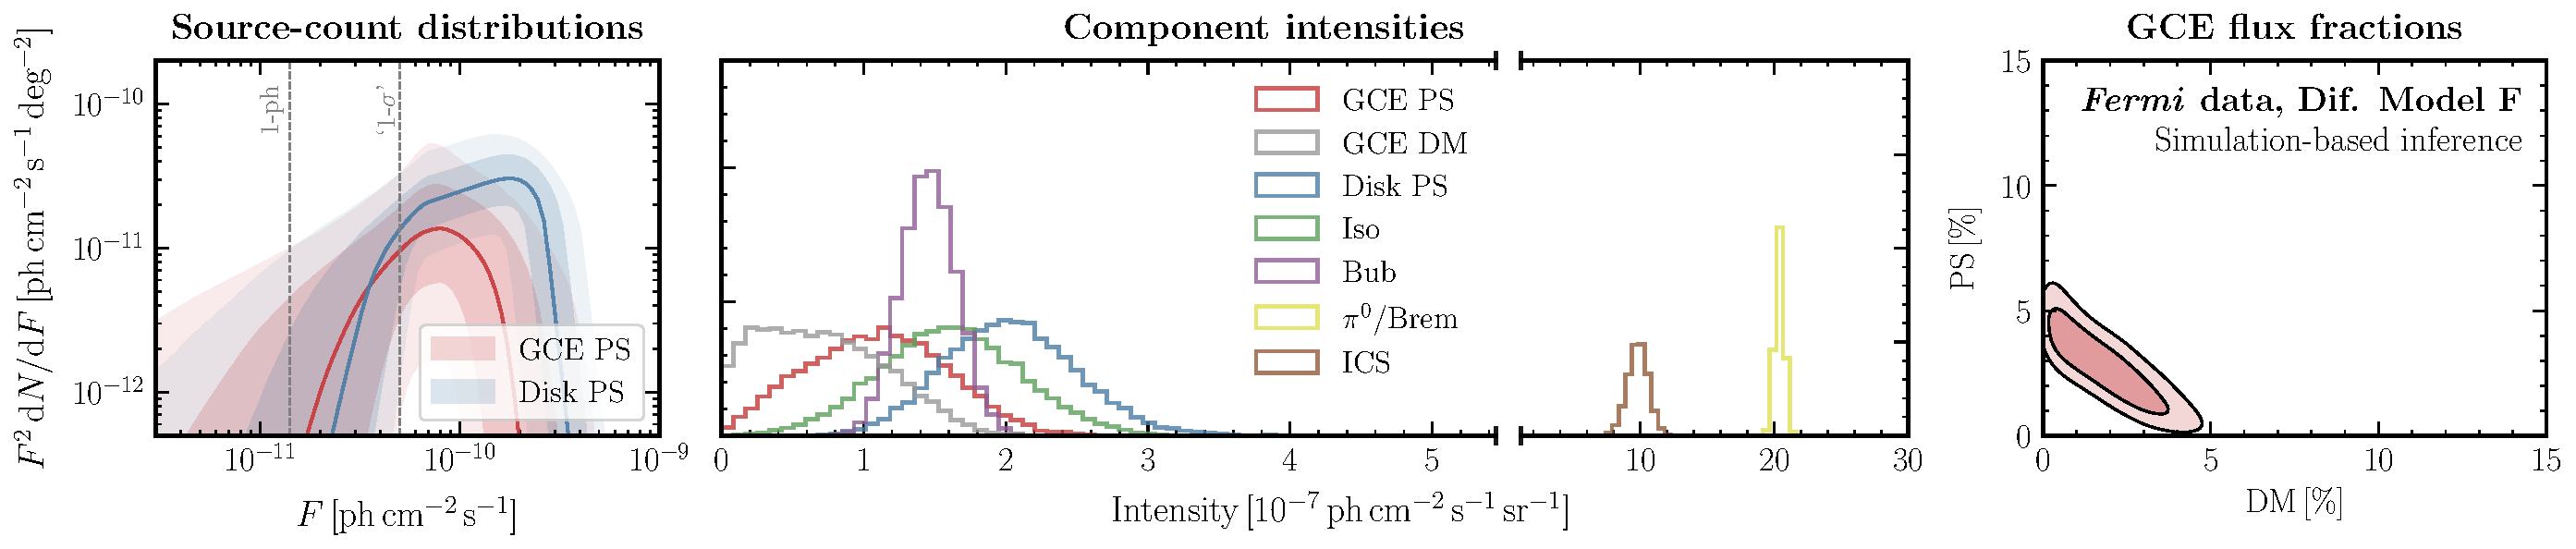
\includegraphics[width=0.95\textwidth]{plots/data_fid_sbi_modelF.pdf}
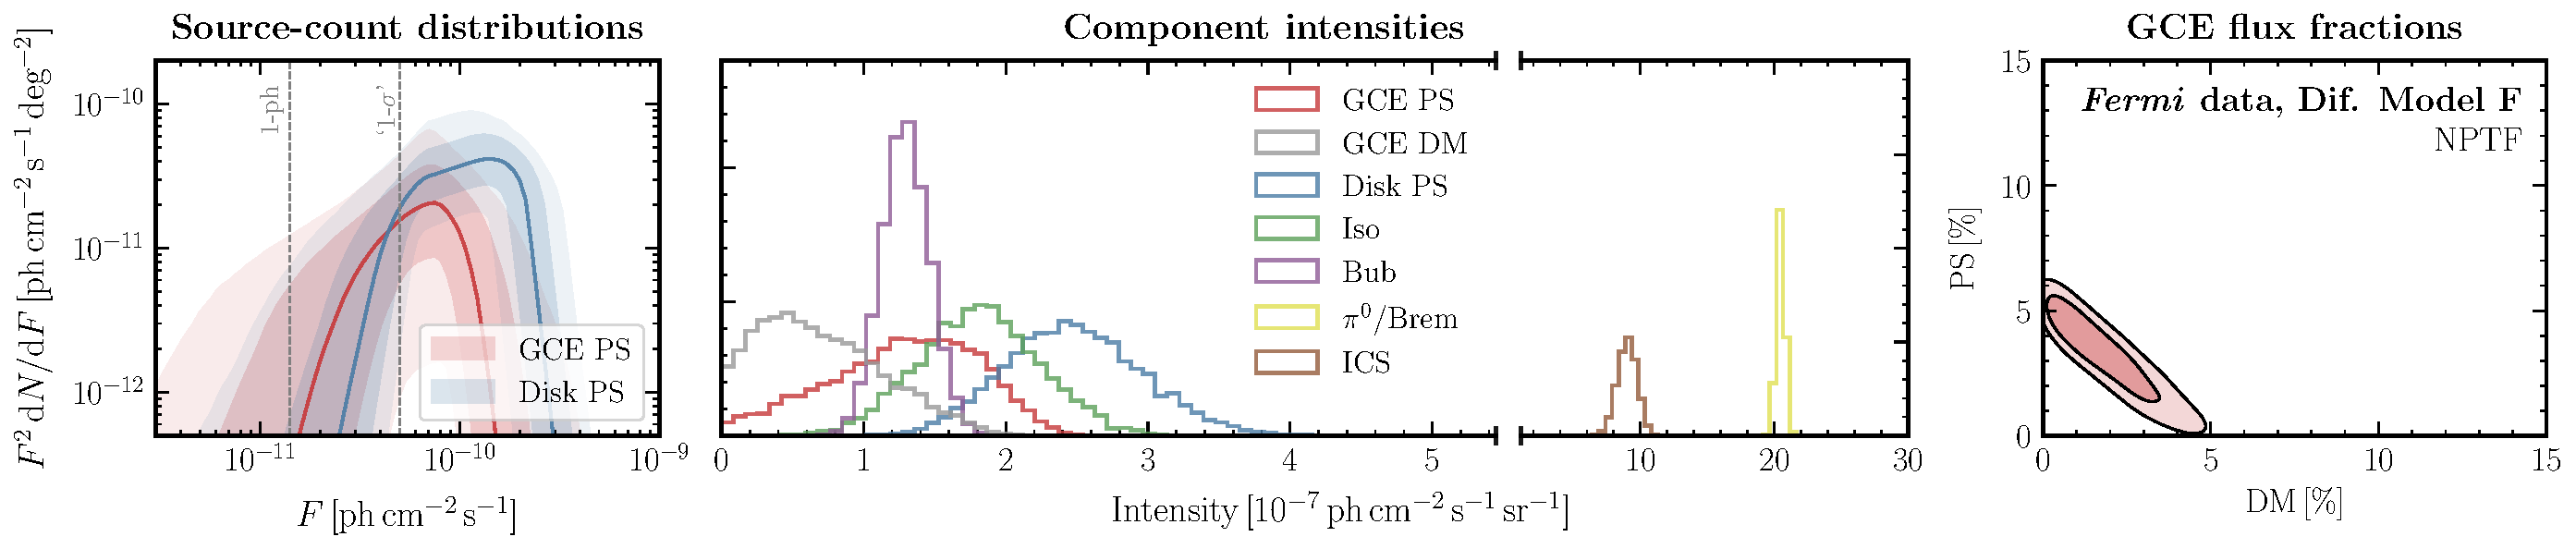
\includegraphics[width=0.95\textwidth]{plots/data_fid_nptf_modelF.pdf}
\caption{Same as Fig.~\ref{fig:fid_data}, but for a model where the diffuse foreground emission is modeled using the alternative Model F.}
\label{fig:fid_data_modelF}
\end{figure*}
%

%
\begin{figure*}
\centering
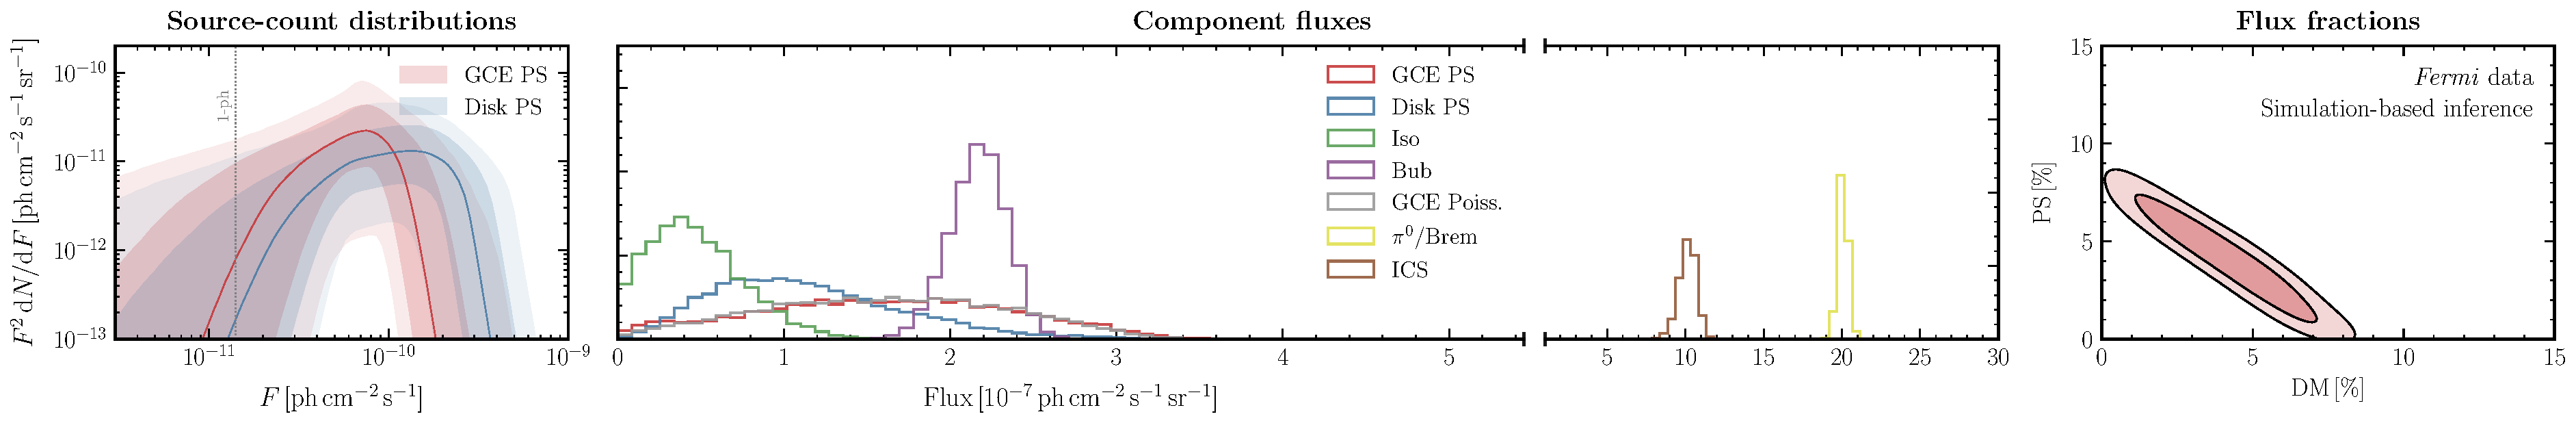
\includegraphics[width=0.95\textwidth]{plots/data_fid_sbi_thick.pdf}
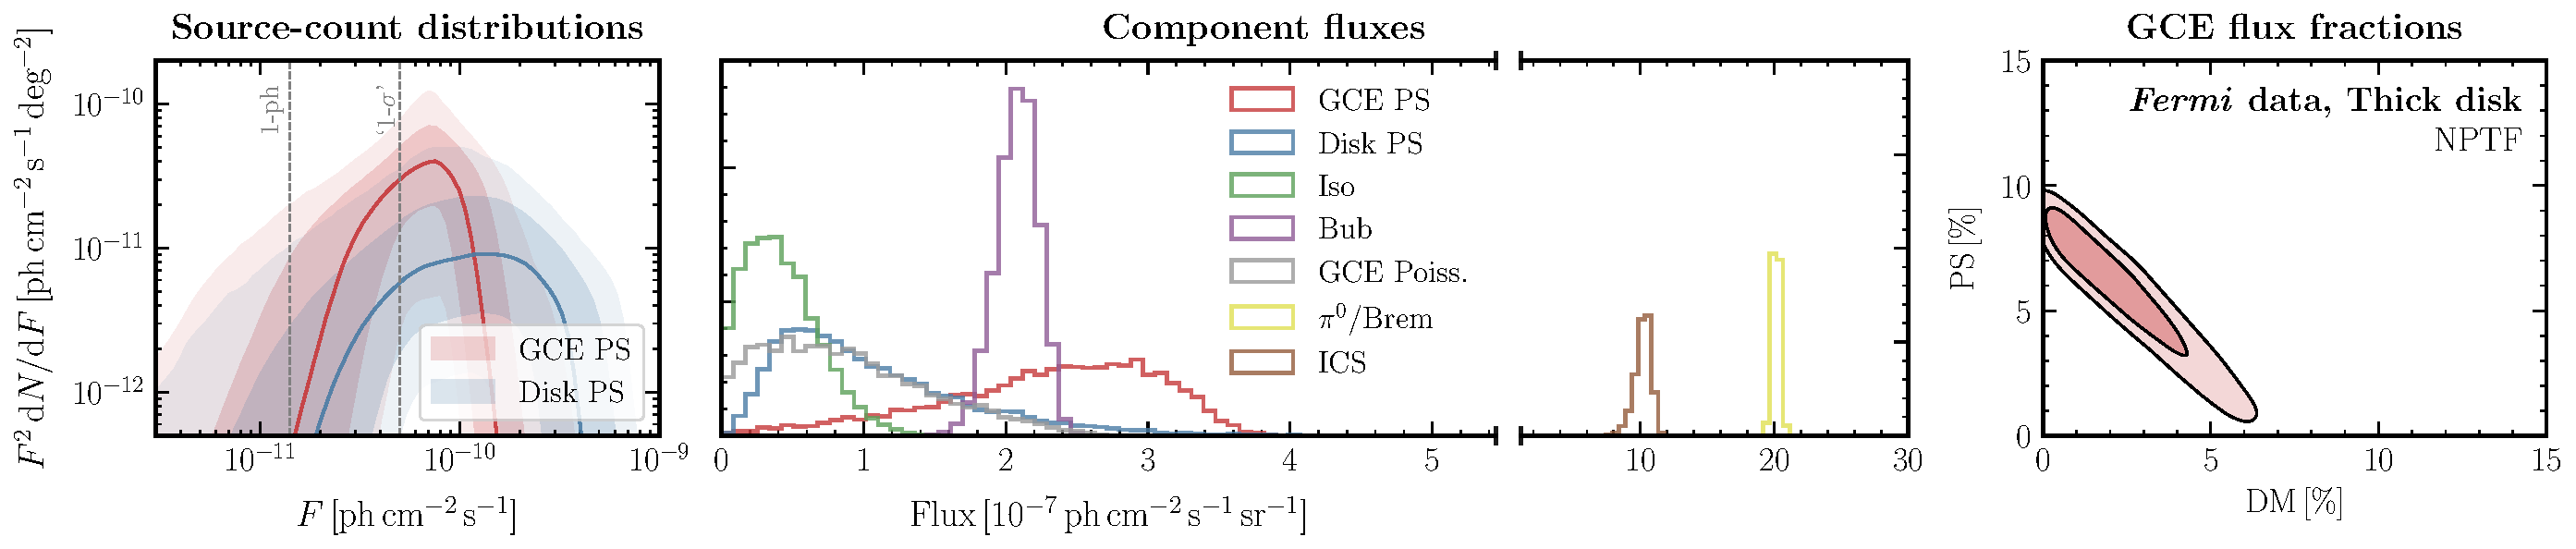
\includegraphics[width=0.95\textwidth]{plots/data_fid_nptf_thick.pdf}
\caption{Same as Fig.~\ref{fig:fid_data}, but for a model where the spatial distribution of disk-correlated PSs is modeled using a thick-disk template (scale factor $z_\mathrm{s}=1\,\mathrm{kpc}$ in Eq.~\eqref{eq:disk_spatial}) rather than the default thin-disk template ($z_\mathrm{s}=0.3\,\mathrm{kpc}$).}
\label{fig:fid_data_thick_disk}
\end{figure*}
%


We test the robustness of our results by exploring several systematic variations on the fiducial analysis, using alternative descriptions for the diffuse foreground emission template and the spatial distribution of disk-correlated sources. Results of these variations are summarized in Tab.~\ref{tab:results}. \\

\noindent
\textbf{Variation on the diffuse foreground model:}
In addition to diffuse Model O considered in the fiducial analysis, we consider the alternative Models A and F from Ref.~\cite{Calore:2014xka} to model the diffuse foreground emission, again including separate templates for gas-correlated emission and inverse Compton scattering. While formally a worse fit to the present dataset~\cite{Buschmann:2020adf}, these models have been previously used in the GCE literature~\cite{Buschmann:2020adf,Leane:2020pfc,Leane:2020nmi} and provide a useful comparison point.

Results for these variations are shown in Figs.~\ref{fig:fid_data_modelA} and \ref{fig:fid_data_modelF}, respectively. In each case, results using the SBI pipeline are shown in the top row, with corresponding results using the NPTF pipeline in the bottom row. 
Qualitatively similar results are obtained when using Model A (Fig.~\ref{fig:fid_data_modelA}) compared to the fiducial analysis in Fig.~\ref{fig:fid_data} using Model O, with $38.9^{+10.2}_{-21.2}\%$ of the GCE flux attributed to PS, roughly half the amount found by the NPTF analysis. Using Model F on the other hand, $52.9^{+10.8}_{-26.1}\%$ of the emission is attributed to PSs, with a marginally larger amount found by the NPTF analysis. The total emission absorbed by the GCE is about half that found in the fiducial scenario. This is consistent with the results of Ref.~\cite{Buschmann:2020adf}, which found that the total GCE flux could vary by a factor of $~2$ between diffuse models. \\

\noindent
\textbf{Variation on the disk template:}
The fiducial scenario considered a disk-correlated PS population with a spatial distribution given by Eq.~\eqref{eq:disk_spatial}, setting the scale height scale height $z_\mathrm{s} = 0.3\,\mathrm{kpc}$ corresponding to the `thin-disk' scenario. Given uncertainties in the spatial distribution of the disk point source (in particular, millisecond pulsar) population, a `thick-disk' spatial distribution has been employed in the literature as an alternative model~\cite{Lee:2015fea,Leane:2019xiy,Buschmann:2020adf}, where the scale height is typically set to $z_\mathrm{s} = 1\,\mathrm{kpc}$. 

Results using a thick-disk template for the disk-correlated PS population are shown in Fig.~\ref{fig:fid_data_thick_disk}. For the SBI analysis, a larger fraction $49.5^{+9.0}_{-22.8}\%$ of the GCE flux is attributed to a PS population in this case compared to the fiducial scenario, with the GCE flux itself being slightly larger. Once again, the NPTF analysis estimates a higher $75.0^{+7.1}_{-22.6}\%$ fraction of the GCE in point sources.\\

% \noindent
% \textbf{Variation of the ROI size:}
% Although the GCE signal is concentrated predominantly in the inner $10^\circ$, the use of the larger $25^\circ$ ROI in this work is motivated by the fact that a larger region may better constrain various spatially-extended modeled emission components. On the other hand, there is also the potential for more susceptibility to mismodeling effects when using a larger ROI. The right panel of Fig.~\ref{fig:variations} shows analysis results using smaller ROI sizes---$10^\circ, 15^\circ$ and $20^\circ$. These are seen to be completely consistent with the fiducial analysis in the $25^\circ$ ROI, with a wider posterior in the smaller ROIs as expected since these contain less information than fiducial ROI.

\section{Susceptibility to mismodeling}
\label{sec:mismodeling}

A key challenge in $\gamma$-ray analyses of the Galactic Center is that associated with effects of mismodeled signal and background templates. As explored in detail in Refs.~\cite{Lee:2015fea,Leane:2020pfc,Leane:2020nmi,Buschmann:2020adf,Chang:2019ars} within the NPTF framework, mismodeling can hamper the characterization of an Inner Galaxy PS population and, if sufficiently severe, can result in the attribution of mismodeled residuals to a spurious PS population when the underlying emission is actually smooth in nature. 

In this section we assess the susceptibility of our simulation-based inference pipeline to systematic mismodeling of the signal and background. We do so by simulating mock data with a smooth GCE signal, additionally containing known mismodeling, and analyzing it with our fiducial pipeline. The ability of our method to correctly characterize the injected signal is then indicative of the level of misattribution that can be expected in the real data under corresponding circumstances. Results for the various tests performed are shown in Fig.~\ref{fig:sim_sbi_mismo}, and will be described below. In each case, we show posteriors by combining samples over 10 different mismodeled templates in order to characterize the `average' mismodeling associated with a given configuration. The first row of Fig.~\ref{fig:sim_sbi_mismo} shows the aggregate analysis without mismodeling \emph{i.e.}, using mock data created with the same templates used in the analysis, as a point of comparison. In all cases tested, while posteriors for certain templates can show systematic biases, preference for a smooth GCE remains robust and PS-like emission is compatible with zero (right-most column of Fig.~\ref{fig:sim_sbi_mismo}). \\

\noindent
\textbf{Test of diffuse mismodeling using an alternative template:}
We create mock data using diffuse Model A, and analyze it using our fiducial analysis pipeline with Model O. The aggregated results over 10 different maps are shown in the second row of Fig.~\ref{fig:sim_sbi_mismo}. We see that while the marginalized DM posterior faithfully corresponds to the true underlying value, the PS template picks up small amount of residual flux. \\

\noindent
\textbf{A data-driven test of large-scale mismodeling:}
In order to test the effect of large-scale foreground mismodeling, we construct a data-driven model of such mismodeling and assess the ability of our method to recover either smooth or PS-like emission in the face of such mismodeling.  Following Ref.~\cite{Mishra-Sharma:2020kjb}, we perform a Poissonian template analysis on the \Fermi dataset $x$, modulating the diffuse model template $T_{\mathrm{dif}}$, which describes the bremsstrahlung and neutral pion decay components of diffuse Model O, by an (exponentiated) Gaussian process (GP):
\begin{equation}
x \sim \operatorname{Pois}\left(\sum_{i \neq \mathrm{dif}} A_{i} T_{i}+\exp \left(f\right) A_{\mathrm{dif}} T_{\mathrm{dif}}\right).
\end{equation}
The other Poissonian templates $T_{i}$, including a GCE DM template and the inverse Compton component of the diffuse foreground model, are treated as before using an overall normalization factor $A_{i}$. $f \sim \mathcal{N}(m, K)$ is the GP component with mean $m$ set to zero, and the covariance $K$ described through the Mat\'ern kernel with smoothness parameter $\nu = 5/2$. We refer to Ref.~\cite{Mishra-Sharma:2020kjb} for further details of the analysis, as well a validation of the GP-augmented template fitting pipeline on simulated data.

%
\begin{figure*}
\centering
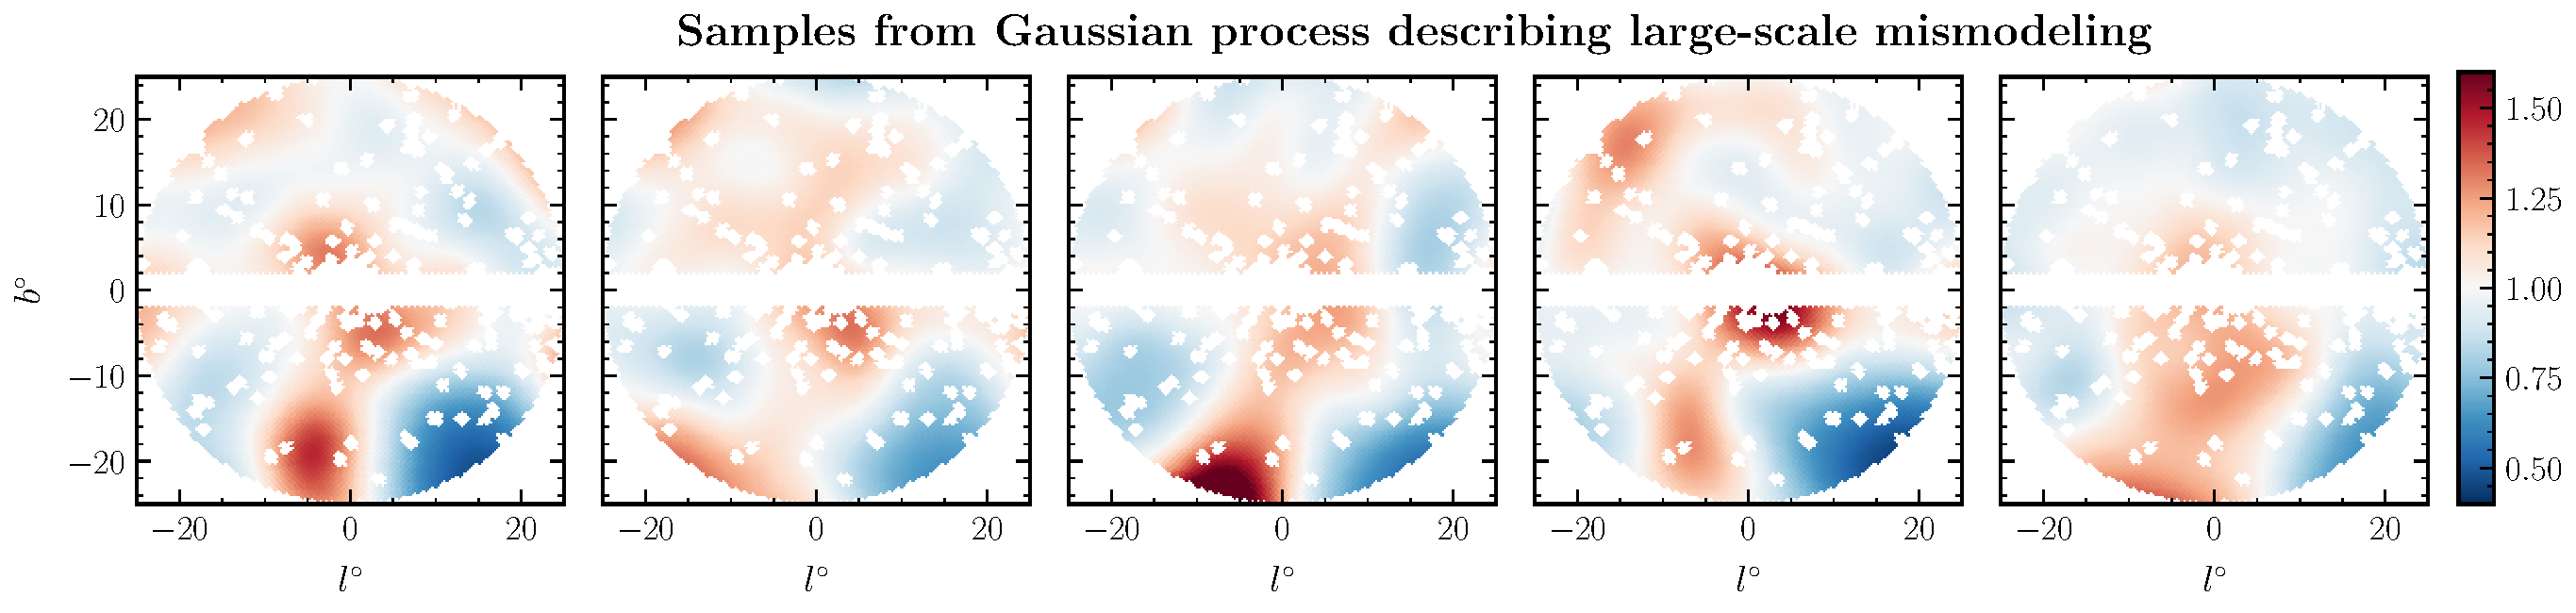
\includegraphics[width=0.95\textwidth]{plots/dd_mismo_map.pdf}
\caption{Fair samples from the Gaussian process description of multiplicative mismodeling associated with diffuse foreground Model O when applied to the real \Fermi data.}
\label{fig:dd_mismo_map}
\end{figure*}
%

Five fair samples from the Gaussian process describing multiplicative mismodeling relative to the real \Fermi data when using our fiducial diffuse Model O are shown in Fig.~\ref{fig:dd_mismo_map}. The largest mismodeling by magnitude in this case is inferred to be concentrated in the southern regions of the fiducial ROI. We note that the recovered GCE flux tends to be lower by up to 40\% when using the GP-modulated diffuse model compared to that obtain in a Poissonian fit, indicating that parts of the centrally concentrated emission could be better described by the modulated template rather than the generalized NFW template modeling DM annihilation. We leave a detailed study of implications of this fact for the morphology of the excess to future work.

In order to test the effect of such mismodeling on recovery of a DM signal we modulate the bremsstrahlung and neutral pion decay-tracing components of Model O using samples drawn from the inferred Gaussian process. These simulated samples are then analyzed with our standard pipeline, using the unmodulated Model O to model the diffuse emission.

The results of this test are shown in the third row of Fig.~\ref{fig:sim_sbi_mismo}. It can be seen that while large-scale mismodeling can distort the total flux attributed to DM-like emission, preference for a smooth origin of the signal remains robust. The DM flux tends to be overestimated however, which may be attributed to the centrally-concentrated mismodeling as seen in Fig.~\ref{fig:dd_mismo_map}. This is also reflected in the fact that the inferred inverse Compton flux tends to be underestimated, with the residual flux attributable to the DM template. \\

% %
% \begin{figure*}
%     \centering
%     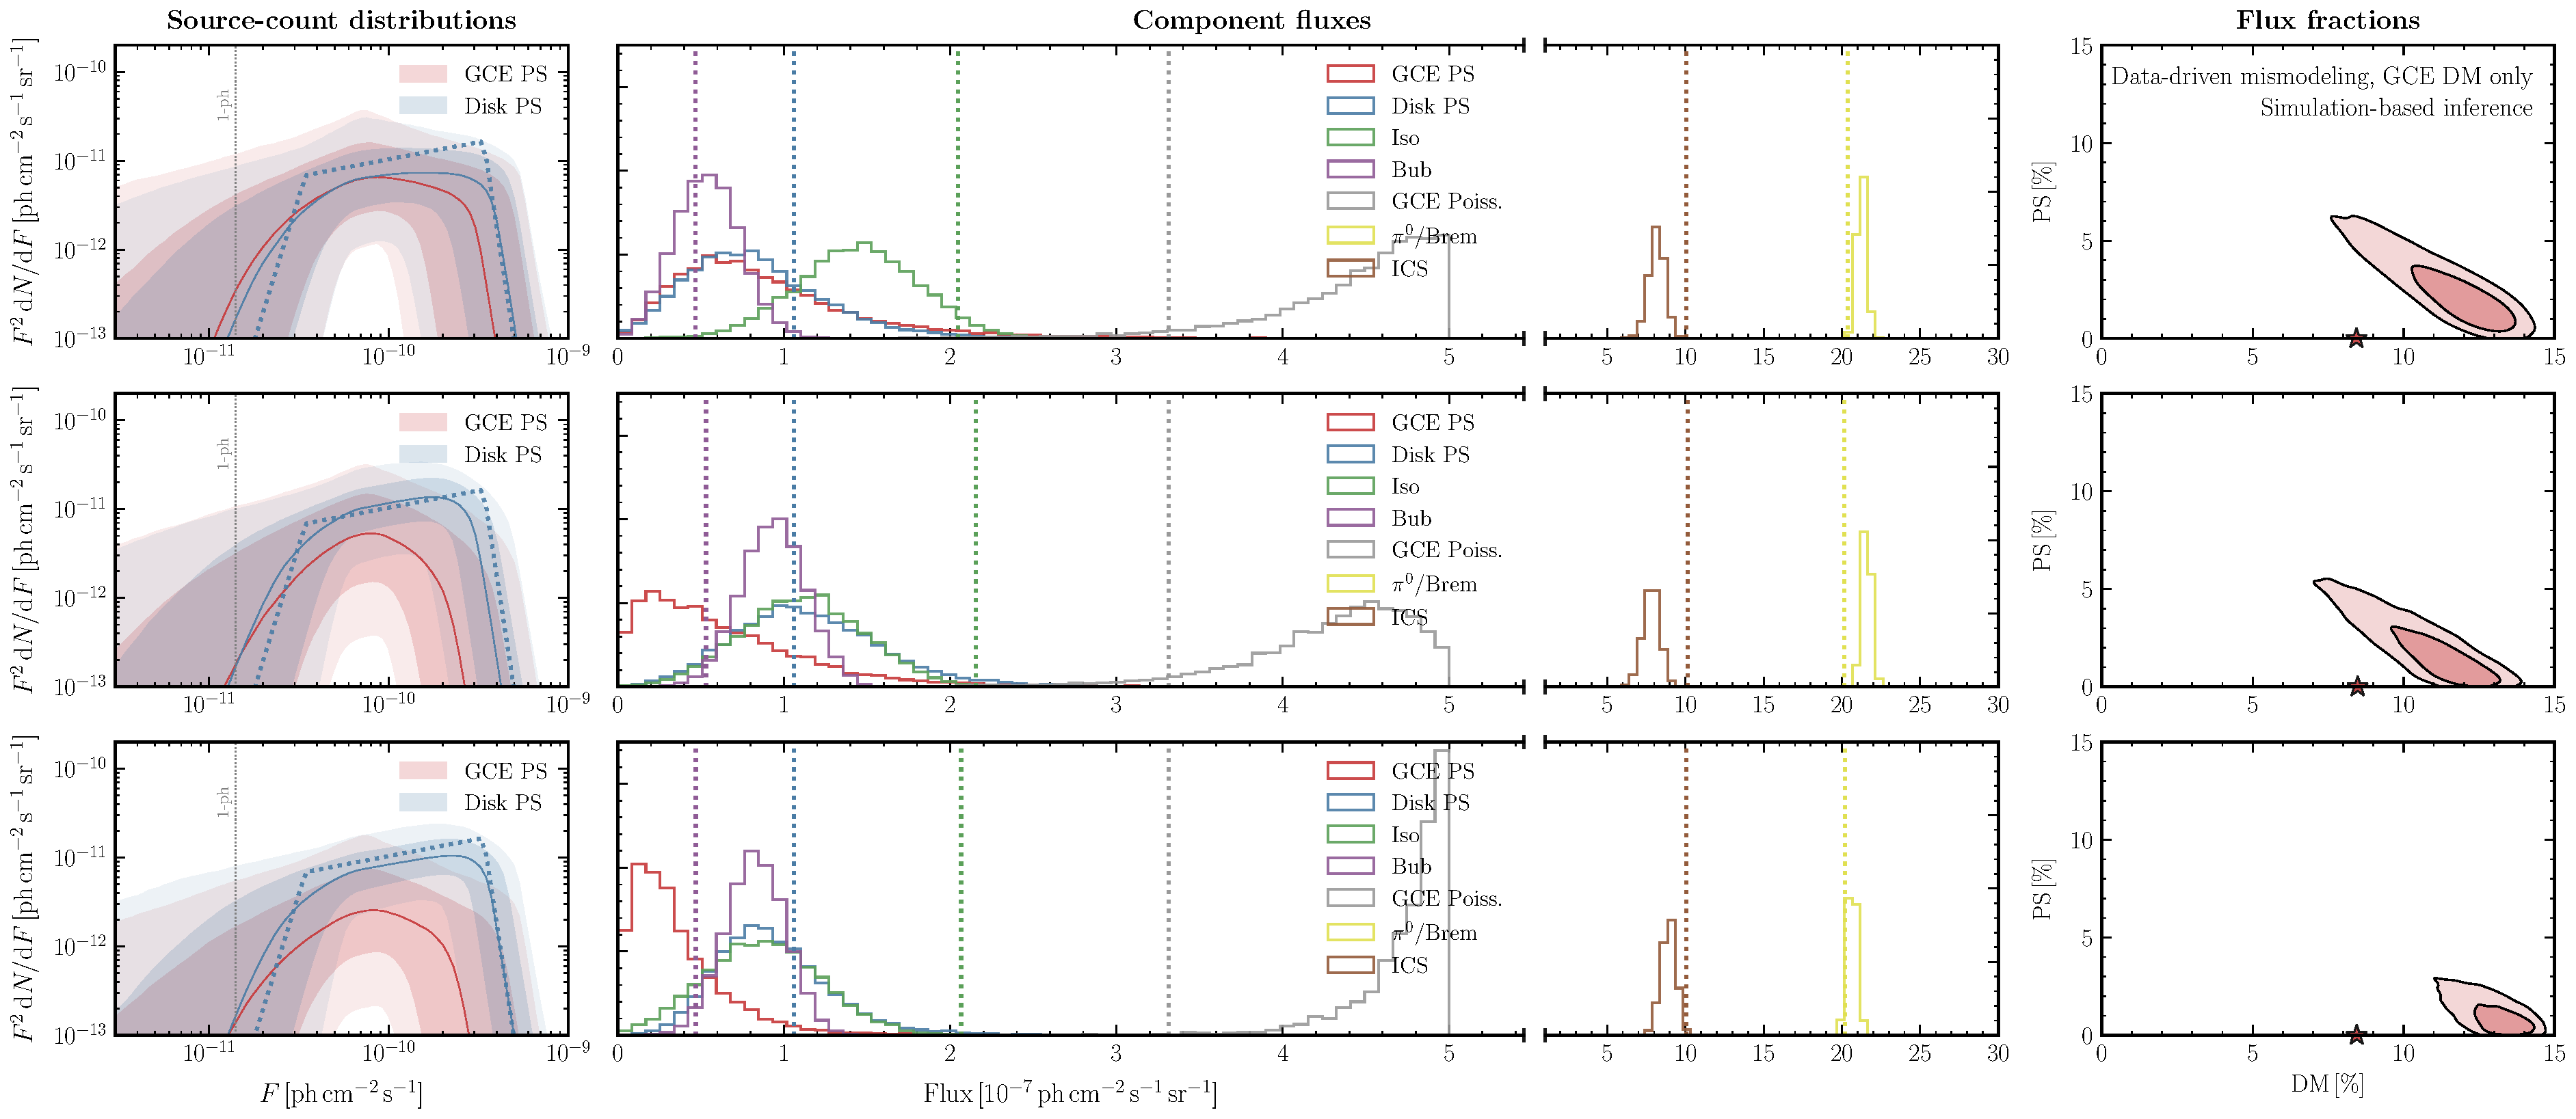
\includegraphics[width=0.95\textwidth]{plots/sim_sbi_dm_mismo.pdf}
%     \caption{Same as Fig.~\ref{fig:sim_sbi_dm}, but for simulated data where the GCE consists of purely DM-like emission and the diffuse model is modulated by draws from the Gaussian process description of diffuse mismodeling. DM-like emission is inferred in each case, although the magnitude of emission is overestimated as some of the diffuse mismodeling is absorbed into the Poissonian GCE component.}
%     \label{fig:sim_sbi_dm_mismo}
% \end{figure*}
% %

%
\begin{figure*}
\centering
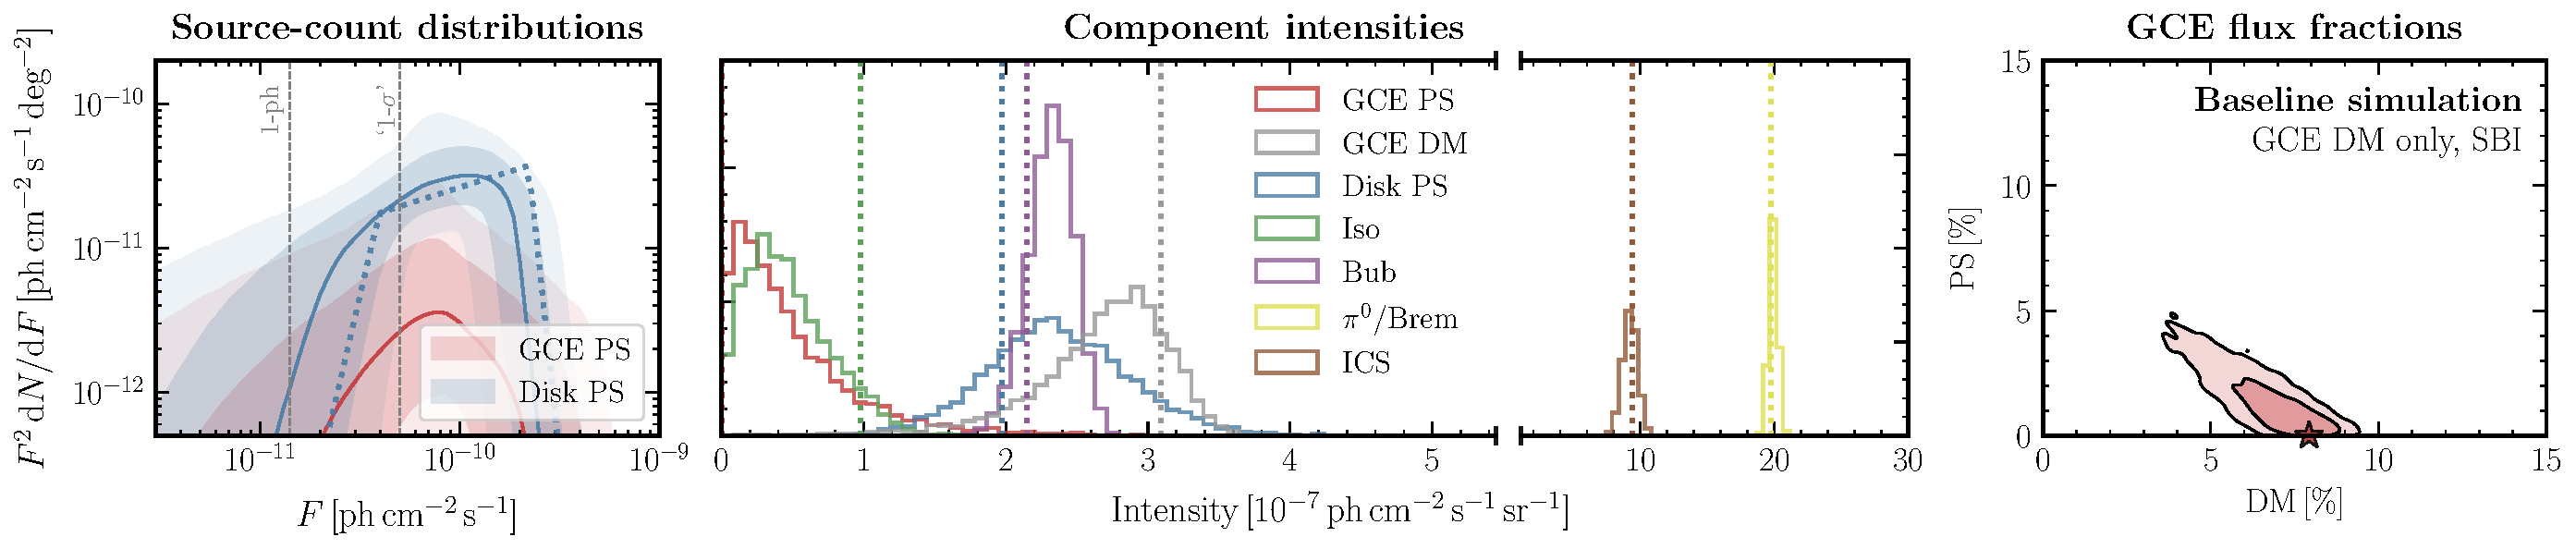
\includegraphics[width=0.95\textwidth]{plots/sim_sbi_dm_agg.pdf}
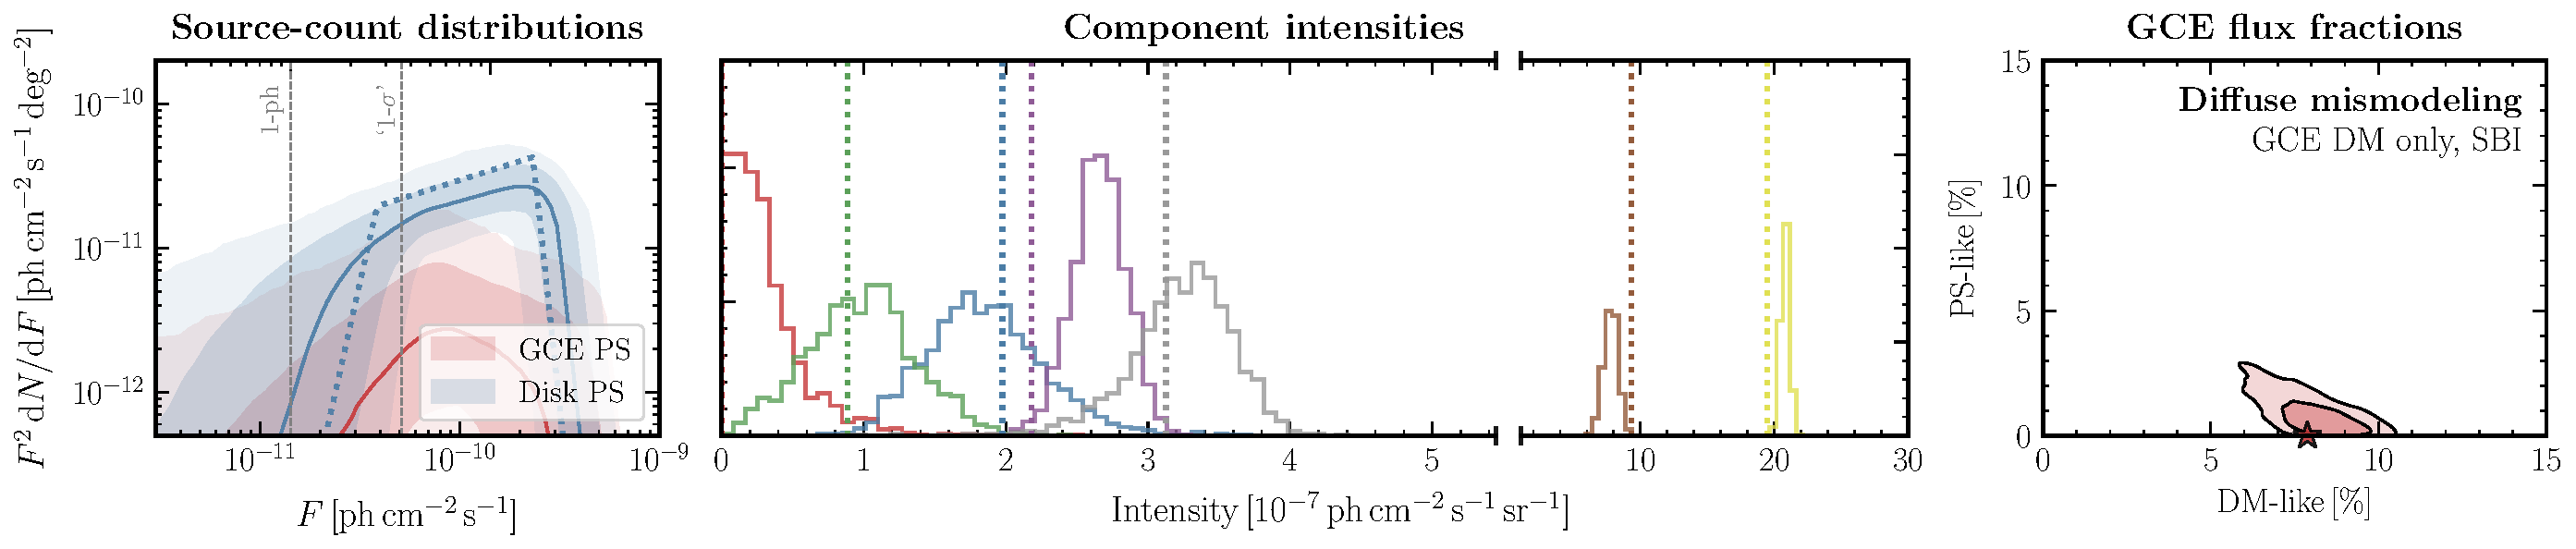
\includegraphics[width=0.95\textwidth]{plots/sim_sbi_modelA_dm.pdf}
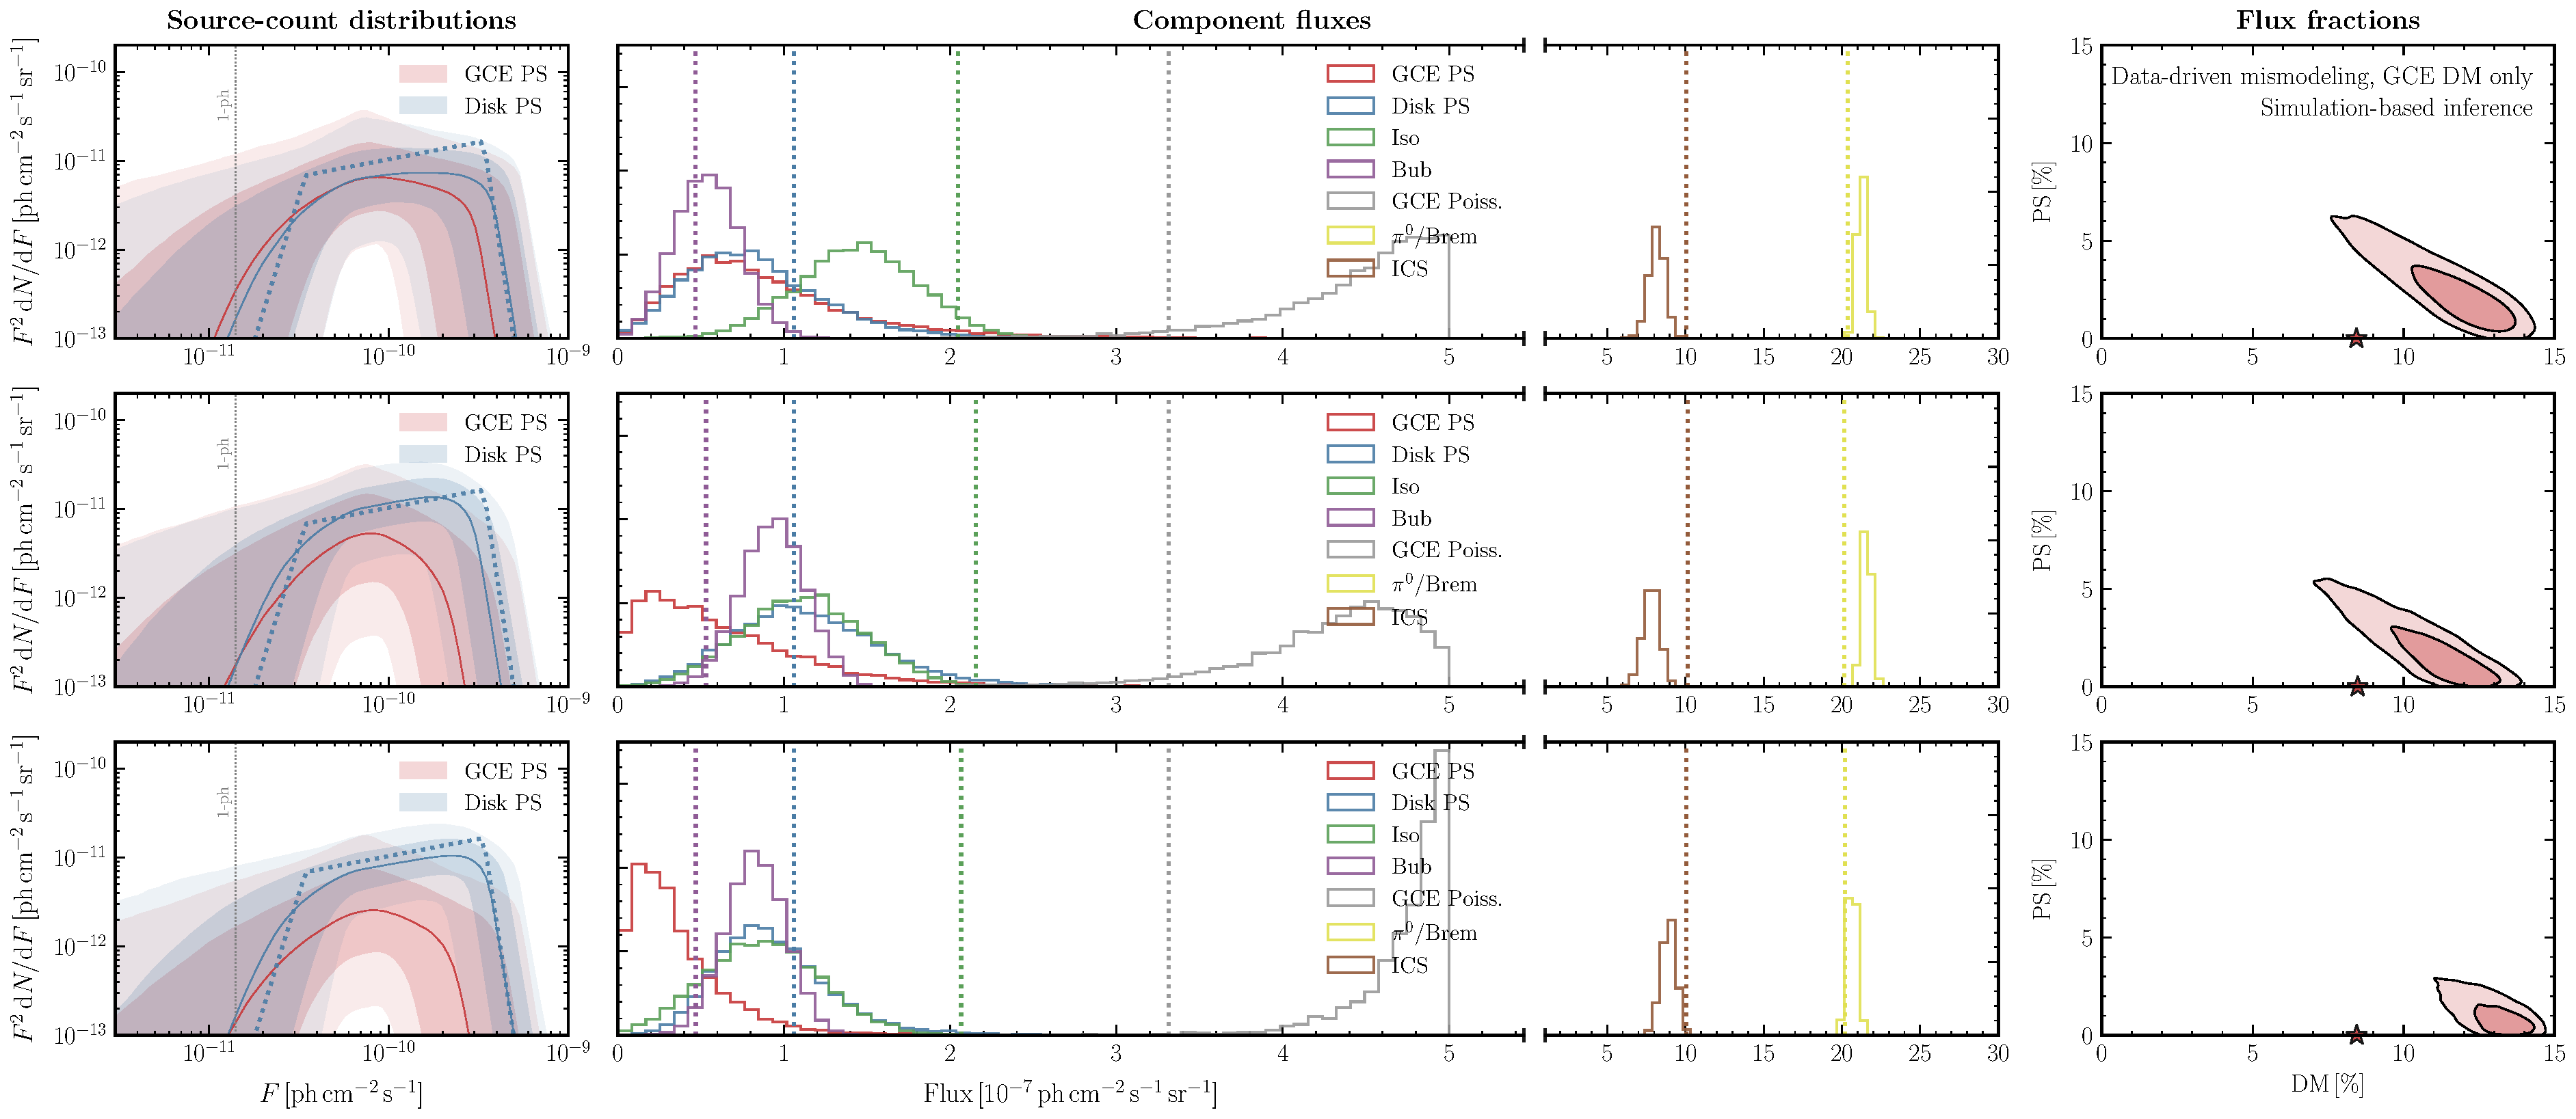
\includegraphics[width=0.95\textwidth]{plots/sim_sbi_dm_mismo.pdf}
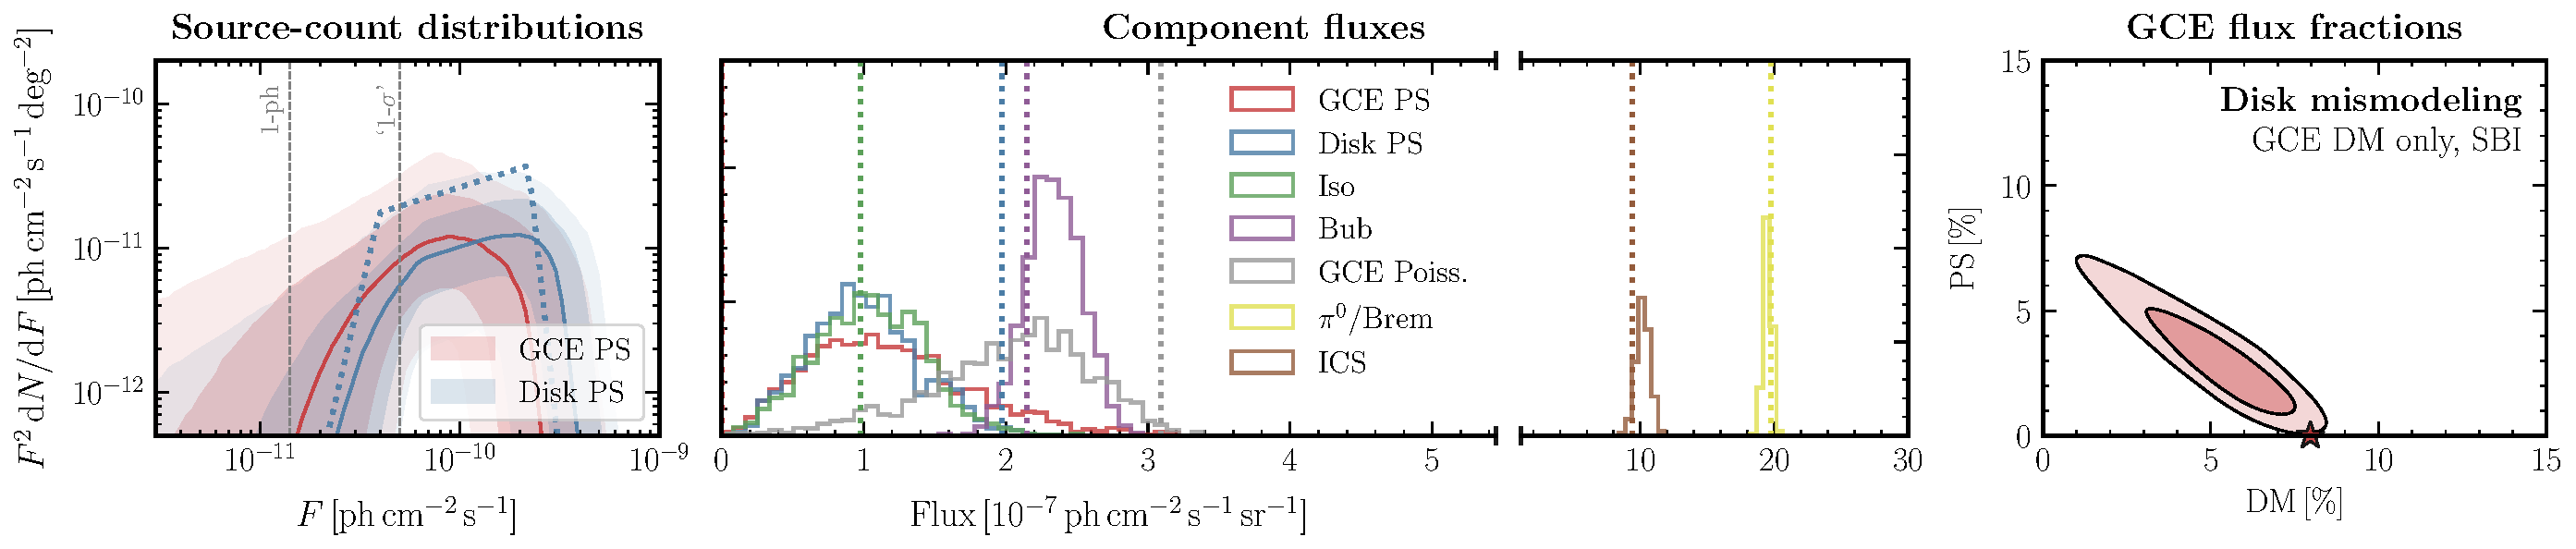
\includegraphics[width=0.95\textwidth]{plots/sim_sbi_thick_disk_mm_dm.pdf}
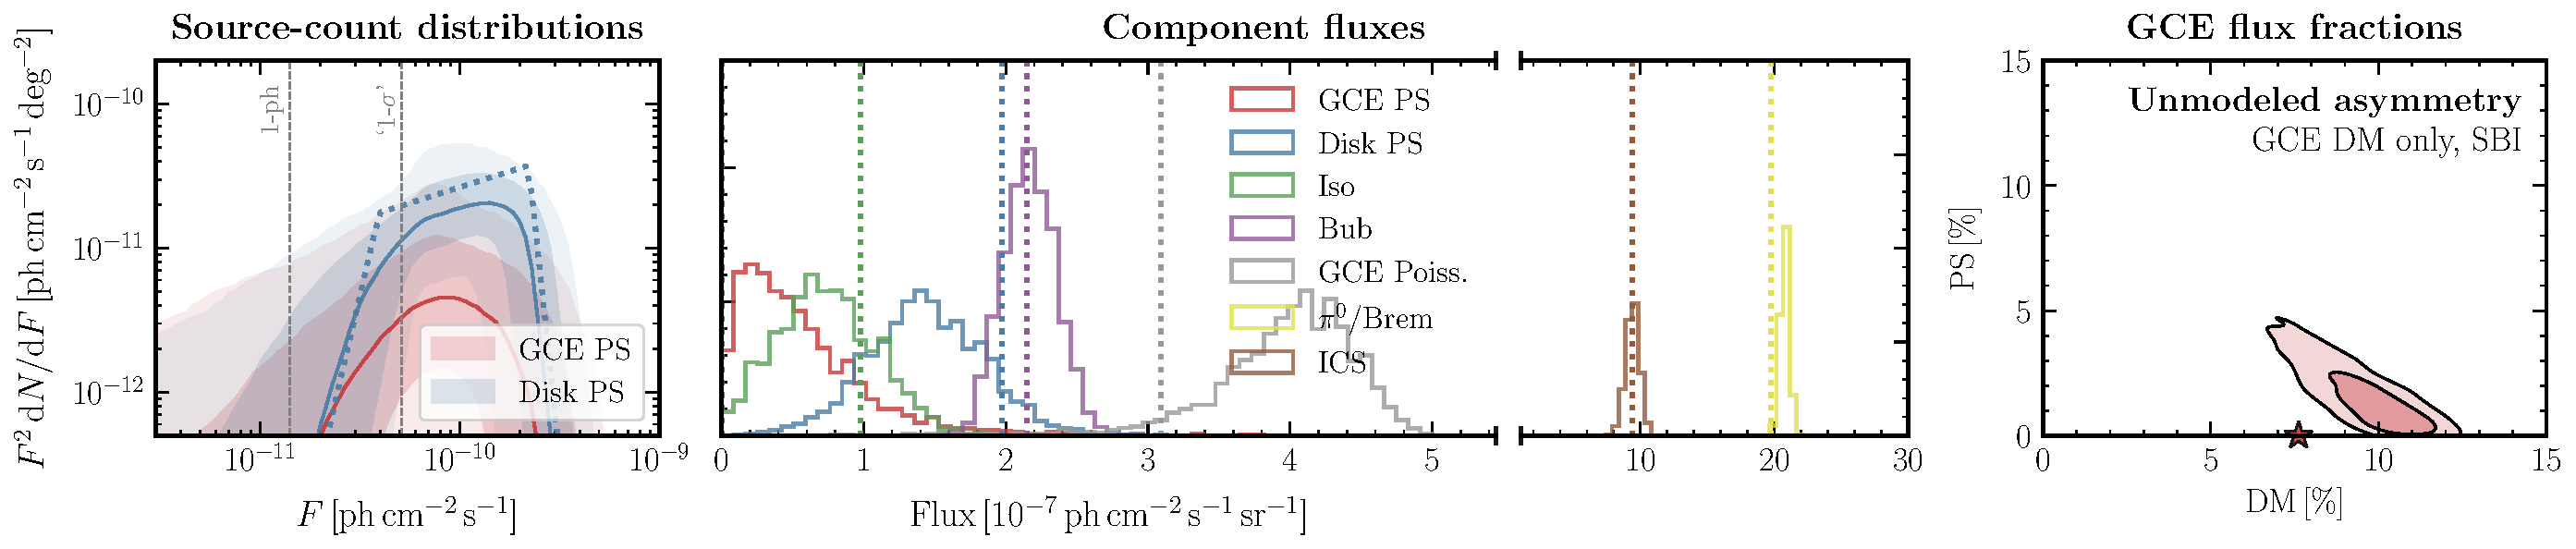
\includegraphics[width=0.95\textwidth]{plots/sim_sbi_dm_asym.pdf}
\caption{Effect of mismodeling on a smooth GCE within our analysis framework. Each row shows aggregate posteriors collected over 10 simulated samples; row-wise from top to bottom: \emph{(i)} No mismodeling; simulated data is constructed with the same templates as those used in the forward model. \emph{(ii)} Mock data created with diffuse Model A, showing the effect of diffuse mismodeling. \emph{(iii)} Mock data where the diffuse template, described by Model O, is modulated by draws from a Gaussian process modeling large-scale mismodeling inferred from the real \Fermi data. \emph{(iv)} Mock data where the thick-disk template is used in lieu of the thin-disk template. \emph{(v)} Mock data where the GCE signal in the Northern hemisphere is twice as large as that in the Southern hemisphere. While some PS-like emission is inferred, it is consistent with zero in all cases, and evidence for a smooth GCE is robust.}
\label{fig:sim_sbi_mismo}
\end{figure*}
%

\noindent
\textbf{Effect of mismodeling the disk spatial template:} 
We replace the thin-disk template, described by a scale height $z_\mathrm{s} = 0.3\,\mathrm{kpc}$ in Eq.~\eqref{eq:disk_spatial}, with a thick-disk template with $z_\mathrm{s} = 1\,\mathrm{kpc}$ in simulated data. Results of then analyzing 10 mock maps with the fiducial thin-disk template are shown in the fourth row of Fig.~\ref{fig:sim_sbi_mismo}. While disk mismodeling can distort the inferred SCD away from the true one, the smooth GCE signal is seen to be successfully recovered in this case. \\

\noindent
\textbf{Effect of an unmodeled asymmetry in the signal:}
Besides mismodeling of the diffuse foreground emission, another major potential concern is associated with mismodeling of the signal emission itself. In particular, as pointed out in Refs.~\cite{Leane:2020nmi,Leane:2020pfc}, a North-South asymmetry in a putative dark matter signal, if unaccounted for, could lead to the inference of a spurious PS population associated with the purely smooth, asymmetric signal in the traditional NPTF framework. Refs.~\cite{Leane:2020nmi,Leane:2020pfc} found preference for such a scenario in real \Fermi data, with the GCE signal in the Northern hemisphere a factor of $\sim2$ larger than that in the Southern hemisphere when the GCE template in the two regions is floated separately in a smaller ROI $r < 10^\circ$. In this case, no preference for a PS-like GCE was found in contrast to when a single template was used to model the GCE. 

We test the impact of a North-South-asymmetric dark matter signal within our framework by running our pipeline on simulated datasets where the dark matter-like signal in the Northern hemisphere of the ROI is 2 times larger than that in the Southern hemisphere, mimicking the preference in real data found in Refs.~\cite{Leane:2020nmi,Leane:2020pfc}. The results of this test on 10 such simulated realizations is shown in the last row of Fig.~\ref{fig:sim_sbi_mismo}. We see that the presence of a substantially asymmetric DM signal has only a marginal impact on the inferred posteriors, and does not lead to a spurious preference for a PS population as was found in the NPTF framework. We attribute this to the fact that the \texttt{DeepSphere}-based feature extractor can account for pixel-to-pixel correlations in the $\gamma$-ray counts map, and can thus be sensitive to \emph{local} PS-like structures. In contrast, the 1-point PDF-based NPTF framework, being agnostic to the ordering of the pixels, can notice spurious PS-like structures in the ``residuals'' associated with an asymmetric signal when analyzed with a symmetric template.
As in Ref.~\cite{Buschmann:2020adf}, we emphasize that the presence of an asymmetry in the GCE signal, if not attributed to diffuse mismodeling, would point towards astrophysical explanations of the GCE since a true dark matter signal would not be expected to be significantly asymmetric.

% %
% \begin{figure*}
%     \centering
%     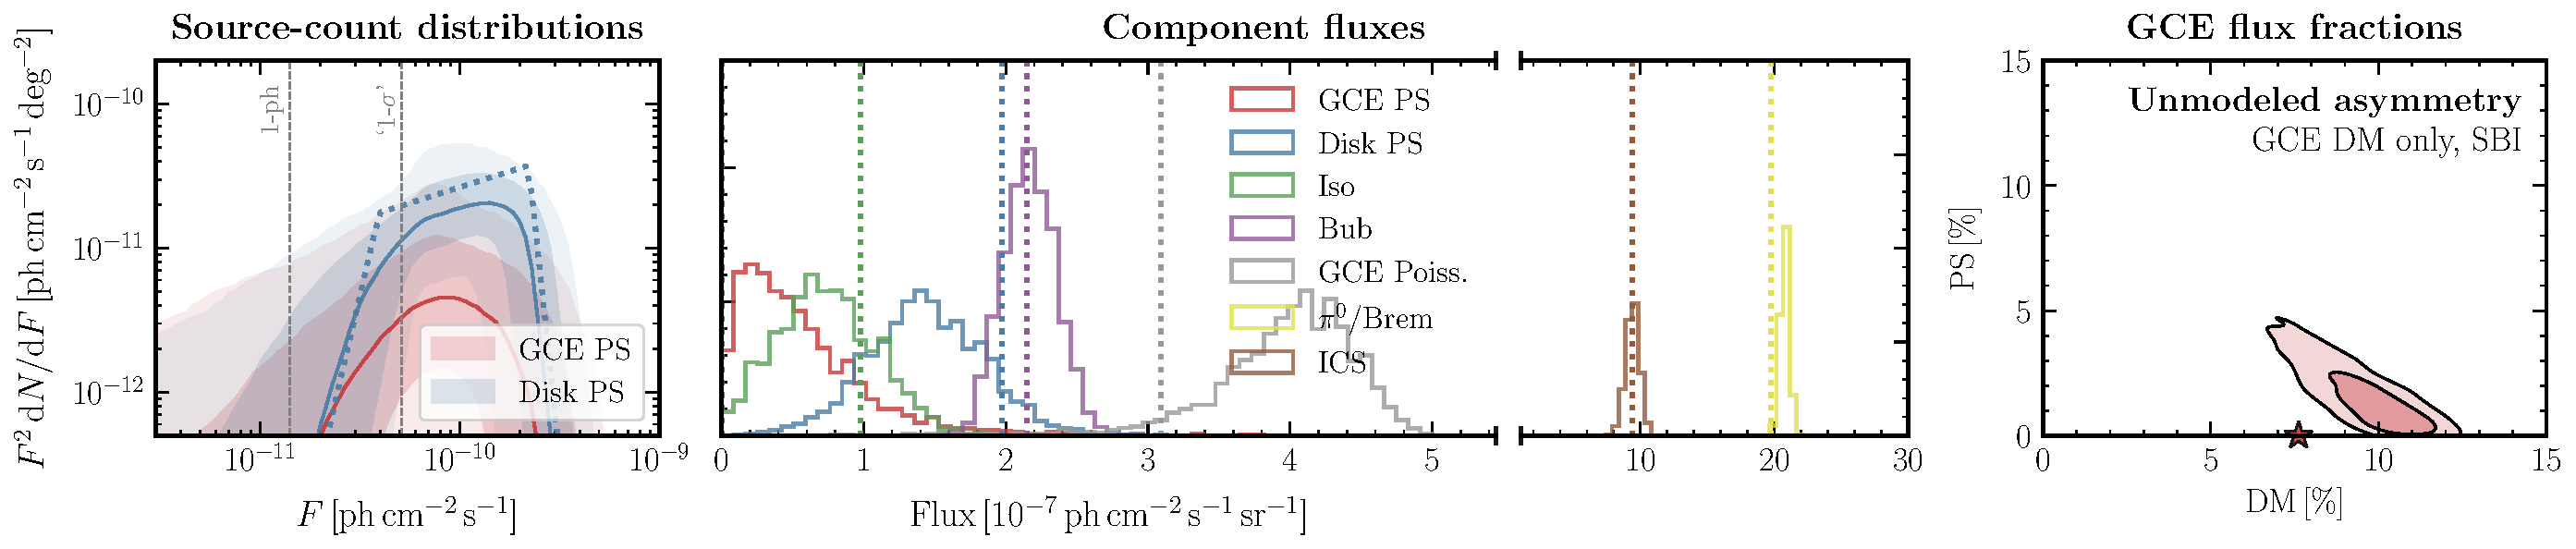
\includegraphics[width=0.95\textwidth]{plots/sim_sbi_dm_asym.pdf}
%     \caption{Same as Fig.~\ref{fig:sim_sbi_dm}, but for simulated data where the GCE consists of purely DM-like emission with a North-South asymmetry; the signal in the Northern hemisphere is larger by a factor of 3. The mismodeled signal is seen to have marginal qualitative effect on the recovery of DM-like emission.}
%     \label{fig:sim_sbi_dm_asym}
% \end{figure*}
% %

\section{Discussion and Conclusions}
\label{sec:conclusion}

In this paper, we have leveraged recent advances in neural simulation-based inference in order to characterize a putative point source population that may be responsible for the observed \Fermi Galactic Center Excess. Consistent with Ref~\cite{List:2020mzd} which used Bayesian neural networks and first leveraged the \texttt{DeepSphere} graph-based architecture for analyzing $\gamma$-ray data, our analysis based on conditional posterior density estimation with normalizing flows shows a reduced preference for an unresolved PS population as the explanation for the GCE compared to previous analyses based on the photon statistics of the $\gamma$-ray map (non-Poissonian template fitting). In particular, depending on the analysis configuration, we find a median value of $\sim30$--$50\%$ as the fraction of GCE emission that can be attributed to a PS population, with the inferred source-count distribution peaking at smaller fluxes $\sim2$--$3\times 10^{-11}$\,ph\,cm$^{-2}$\,s$^{-1}$ compared to values found in previous analyses based on the non-Poissonian template fitting (NPTF) framework~\cite{Lee:2015fea}, where the SCD is seen to peak just below the threshold for resolution of individual PSs, roughly $\sim2\times 10^{-10}$\,ph\,cm$^{-2}$\,s$^{-1}$. The NPTF analyses performed in this work find a similarly dim source-count distribution, in all cases however attributing a larger fraction $\sim50$--$75\%$ of the GCE to a PS population as compared to the corresponding SBI analyses.

Our qualitative conclusions are robust to the systematic variations we have explored, including variations on the the diffuse foreground model and spatial modeling of disk-correlated PS emission. We used a novel Gaussian process-based method to construct a data-driven model of large-scale mismodeling, finding our method to be resilient to such mismodeling when it comes to differentiating between a smooth and PS-like GCE. As in any Galactic Center $\gamma$-ray analysis, given the poorly understood astrophysical emission in this region, we caution of the potential of unknown systematics, such as mismodeling on the scale of the size of the \Fermi-LAT point-spread function, to bias the results and conclusions of our analysis.

Several improvements to the framework presented here are possible. The inclusion of energy-binning information in the analysis can be implemented by splitting up the data and template maps into individual bins and feeding these as separate channels in the graph-convolutional feature extraction network. The use of more complex feature extraction and flow architectures can additionally improve the robustness of our results. 

Since diffuse mismodeling is the largest source of uncertainty in any analysis that aims to characterize the GCE, we also note the possibility of using adversarial learning methods~\cite{Louppe:2016ylz} to account for systematic differences between the modeled and real \Fermi data. Alternatively, generative modeling of the diffuse foreground either in a Gaussian process-based data-driven framework or using, \emph{e.g.}, autoencoders trained on an ensemble of plausible diffuse models, can provide a principled way to account for the large latent space associated with diffuse emission modeling. Similarly, motivated by quantitative variations in our results on \Fermi data when using different disk templates, self-consistently accounting for plausible variations in the spatial distribution of disk-correlated PSs can strengthen the results of our analysis when it comes to characterizing the PS population in the Galactic Center. 

While we have considered a simulated-based inference framework based on posterior density estimation with normalizing flows, alternative frameworks based on likelihood-ratio estimation~\cite{Brehmer:2018eca,Brehmer:2018hga,Brehmer:2018kdj,Cranmer:2015bka, Hermans:2019ioj,Miller:2020hua,Miller:2021hys} or flow-based likelihood estimation~\cite{winkler2019learning,papamakarios2019sequential} can provide complementary ways to characterize the $\gamma$-ray PS population in the Galactic Center. Additionally, the use of sequential active-learning methods~\cite{papamakarios2019sequential} and methods that make use of additional latent information from the simulator~\cite{Brehmer:2018eca,Brehmer:2018hga,Brehmer:2018kdj,Brehmer:2019xox,Stoye:2018ovl} can significantly improve the sample efficiency of simulations and allow for extensions to more complex latent spaces, which will be important in particular for an energy-binned analysis and when including additional degrees of freedom in the astrophysical background models. 
These extensions can lead to a more robust characterization of an unresolved PS population in the Galactic Center region associated with the GCE, and we leave their study to future work.

The code used to obtain the results in this paper is available at \url{https://github.com/smsharma/fermi-flows}.

% \SM{Beef up attribution to previous papers on different topics.}

\vspace{.2cm}
%%%%%%%%%%%%%%%

\begin{acknowledgments}

We thank Johann Brehmer, Florian List, Nick Rodd, and Tracy Slatyer for helpful conversations. 
SM would like to thank the Center for Computational Astrophysics (Flatiron Institute) for their hospitality while this work was being performed. 
This work was performed in part at the Aspen Center for Physics, which is supported by National Science Foundation grant PHY-1607611.
The participation of SM at the Aspen Center for Physics was supported by the Simons Foundation.
KC is partially supported by NSF awards ACI-1450310, OAC-1836650, and OAC-1841471, the NSF grant PHY-1505463, and the Moore-Sloan Data Science Environment at NYU. 
SM is supported by the NSF CAREER grant PHY-1554858, NSF grants PHY-1620727 and PHY-1915409, and the Simons Foundation. 
This work made use of the NYU IT High Performance Computing resources, services, and staff expertise. 
This research has made use of NASA's Astrophysics Data System. 
This research made use of the \texttt{astropy}~\cite{Price-Whelan:2018hus,Robitaille:2013mpa}, \texttt{dynesty}~\cite{Speagle_2020}, \texttt{getdist}~\cite{Lewis:2019xzd}, \texttt{IPython}~\cite{PER-GRA:2007}, Jupyter~\cite{Kluyver2016JupyterN}, \texttt{matplotlib}~\cite{Hunter:2007}, \texttt{MLflow}~\cite{chen2020developments}, \texttt{nflows}~\cite{nflows}, \texttt{NPTFit}~\cite{Mishra-Sharma:2016gis}, \texttt{NumPy}~\cite{harris2020array}, \texttt{pandas}~\cite{pandas:2010}, \texttt{Pyro}~\cite{bingham2018pyro}, \texttt{PyTorch}~\cite{NEURIPS2019_9015}, \texttt{PyTorch Geometric}~\cite{Fey/Lenssen/2019}, \texttt{PyTorch Lightning}~\cite{william_falcon_2020_3828935}, \texttt{seaborn}~\cite{seaborn}, \texttt{sbi}~\cite{tejero-cantero2020sbi}, \texttt{scikit-learn}~\cite{scikit-learn}, \texttt{SciPy}~\cite{2020SciPy-NMeth}, and \texttt{tqdm}~\cite{da2019tqdm} software packages. We acknowledge the use of the code repository associated with Ref.~\cite{List:2020mzd}, in particular the associated data products and templates.\footnote{\url{https://github.com/FloList/GCE_NN}} We acknowledge the use of the code repository associated with Ref.~\cite{defferrard2020deepsphere}, in particular the implementation of the \texttt{DeepSphere} graph convolutional kernel.\footnote{\url{https://github.com/deepsphere/deepsphere-pytorch}}
\end{acknowledgments}

% \appendix

% \section{Variations on analysis}
% \label{app:variations}

\bibliographystyle{apsrev4-1}
\bibliography{fermi-gce-sbi}

\end{document}
